\documentclass[11pt]{report}
\usepackage{titlesec}
\titleformat{\chapter}
{\normalfont\LARGE\bfseries}{\thechapter}{1em}{}
\titlespacing*{\chapter}{0pt}{3.5ex plus 1ex minus .2ex}{2.3ex plus .2ex}

\usepackage[margin=1.2in]{geometry}
\usepackage[toc,page]{appendix}
\usepackage{graphicx}
\usepackage{lipsum}
\usepackage{caption}
\usepackage[utf8]{inputenc}
\usepackage[italian]{babel}
\usepackage{indentfirst}
\usepackage{verbatim}
\usepackage{colorprofiles}
\usepackage{listings}   
\usepackage{float}
\usepackage{subcaption}
\usepackage{amsmath}
\usepackage{amsfonts}
\usepackage{booktabs}
\usepackage{makecell}
\usepackage{xcolor}
\usepackage{textcomp}
\usepackage{gensymb}
\usepackage[hidelinks]{hyperref}

\makeatletter
\renewcommand{\@cite}[2]{{\bfseries[#1\if@tempswa , #2\fi]}}
\makeatother

\newcommand{\reportmaintitle}{Ducted Fan}
\newcommand{\reportsubtitle}{Sviluppo della telemetria, identificazione del modello e simulazione del Double Propeller Ducted-Fan}

\hypersetup{
	pdftitle={Ducted Fan: sviluppo della telemetria, identificazione del modello e simulazione del Double Propeller Ducted-Fan}
}

%%%%%%%%%%%%%%%%%%%%%%%%%%%%%%%%%%%%%%%%%%%%%%%%%%%%%%%%%%%%%%%%%%%%
\definecolor{custom_green}{rgb}{0,0.6,0}
\definecolor{codegray}{rgb}{0.5,0.5,0.5}
\definecolor{custom_blue}{rgb}{0.05,0.05,0.97}
\definecolor{custom_purple}{rgb}{0.58,0.00,0.82}
\definecolor{custom_orange}{rgb}{0.94,0.59,0.09}


\lstdefinestyle{base}{
	language=C,
	backgroundcolor=\color{white},  
	basicstyle=\footnotesize\ttfamily\color{black},   
	breakatwhitespace=false,       
	breaklines=true,               
	columns=fullflexible,
	captionpos=b,                   
	commentstyle=\color{custom_green},   
	inputencoding=utf8,
	extendedchars=true,
	keepspaces=true,
	literate={à}{{\`a}}1 {è}{{\`e}}1 {é}{{\'e}}1 {ì}{{\`i}}1 {ò}{{\`o}}1 {ù}{{\`u}}1 {°}{{\textdegree}}1 {μ}{{$\mu$}}1 {─}{{--}}1 {—}{{--}}1 {→}{{$\rightarrow$}}2,
	escapeinside={\%*}{*)},
	keywordstyle=\color{custom_purple},
	identifierstyle=\color{custom_blue},
	stringstyle=\color{custom_orange},      
	numbers=left,                 
	numbersep=5pt,                  
	numberstyle=\tiny\color{codegray}, 
	rulecolor=\color{black},        
	showspaces=false,               
	showstringspaces=false,        
	showtabs=false,                
	stepnumber=1,                   
	tabsize=4,                     
}

\lstset{style=base}


%%%%%%%%%%%%%%%%%%%%%%%%%%%%%%%%%%%%%%%%%%%%%%%%%%%%%%%%%%%%%%%%%%%%




\begin{document}
	\captionsetup[figure]{margin=1.5cm,font=small,labelfont={bf},name={Figura},labelsep=colon,textfont={it}}
	\captionsetup[table]{margin=1.5cm,font=small,labelfont={bf},name={Tabella},labelsep=colon,textfont={it}}
	
	
	%%%%%%%%%%%%%%%%%%%%%%%%%%%%%%%%%%%%%%%%%%%%%%%%%%%%%%%%%%%%%%%%%%%%
	%                              COPERTINA
	%%%%%%%%%%%%%%%%%%%%%%%%%%%%%%%%%%%%%%%%%%%%%%%%%%%%%%%%%%%%%%%%%%%%
	\begin{titlepage}
		\begin{center}
			\
			\LARGE {\scshape{Università Politecnica delle Marche}}\\[0.5cm]
			\LARGE {\scshape{Laboratorio di Automazione}}\\[0.5cm]
			\LARGE {\scshape{Corso di Laurea Triennale in Ingegneria Informatica e dell'Automazione}}\\[0.7cm]
			\linespread{1}
			
\includegraphics[width=4cm]{images/logoUnivpm.jpg}\\[0.8cm]
			\linespread{1}
			\huge {\bfseries \reportmaintitle}\\[0.4cm]
			{\Large\bfseries\parbox{0.9\textwidth}{\centering \reportsubtitle}}\\[1.2cm]
			\linespread{1.2}
			{\Large Relatori:}
			\hfill {\Large Tesina di:}\\
			\begin{minipage}[t]{0.48\textwidth}
				\raggedright
				{\Large Prof. Bonci Andrea}\\
				{\Large Dott. di Biase Alessandro}
			\end{minipage}
			\hfill
			\begin{minipage}[t]{0.48\textwidth}
				\raggedleft
				{\Large Di Tizio Nicolas}\\
				{\Large Marcucci Simone}\\
				{\Large Morresi Tommaso}\\
				{\Large Nalli Alberto}
			\end{minipage}\\[1.5cm]
			{\Large Anno Accademico 2025/2026}\\[0.5cm]
			{
				
\includegraphics[width=2cm]{images/dii_new.png}\\[0.3cm]
				\large Dipartimento di Ingegneria dell'Informazione\\[0.3cm]
			}
		\end{center}
	\end{titlepage}
	
	\pagenumbering{arabic}
	\tableofcontents
	\addcontentsline{toc}{chapter}{Introduzione}
	\newpage
	
	\pagestyle{plain}
	
	%%%%%%%%%%%%%%%%%%%%%%%%%%%%%%%%%%%%%%%%%%%%%%%%%%%%%%%%%%%%%%%%%%%%
	%                             INTRODUZIONE
	%%%%%%%%%%%%%%%%%%%%%%%%%%%%%%%%%%%%%%%%%%%%%%%%%%%%%%%%%%%%%%%%%%%%
	\section*{Introduzione}
	
	Il presente documento illustra le attività di sviluppo, caratterizzazione e controllo svolte sul prototipo \textit{Double Propeller Ducted-Fan (DPDF)}, un velivolo a propulsione intubata controrotante. Il lavoro ha preso avvio da una necessaria fase di rigenerazione tecnica del prototipo: l'intera struttura meccanica è stata riprogettata e ristampata in 3D, mentre l'elettronica di bordo e i cablaggi sono stati integralmente riassemblati e collaudati.\\
	Il contributo originale del presente lavoro si articola attorno a tre assi principali. Il primo è la realizzazione di un'\textbf{infrastruttura di telemetria} dedicata: il firmware implementato su STM32 NUCLEO-H745ZI-Q trasmette a 50 [Hz], su porta seriale a 230\,400 [baud], un flusso CSV continuo che include angoli di assetto, quota, comandi motori e servo, contatori di errore UART e \textit{flag} di stato. Lo \textit{script} MATLAB \texttt{AcquiringData.m} gestisce lato PC la ricezione, l'archiviazione su file e la generazione in tempo reale dei segnali di eccitazione, rendendo possibile l'acquisizione di \textit{dataset} strutturati senza interruzioni manuali.\\
	Il secondo asse è l'\textbf{identificazione di sistema}. I \textit{dataset} acquisiti durante sessioni di eccitazione PRBS e a gradino sono stati elaborati in MATLAB tramite la funzione \texttt{tfest} del \textit{System Identification Toolbox}, che ha permesso di stimare le funzioni di trasferimento a tempo discreto della risposta di \textit{roll} e \textit{pitch} del velivolo rispetto all'angolo imposto ai rispettivi \textit{flap}. I modelli identificati sono stati utilizzati per la sintesi automatica dei regolatori PIDF tramite \texttt{pidtune} e per la verifica della risposta in anello chiuso in simulazione.\\
	Il terzo asse è lo sviluppo di un \textbf{simulatore fisico tridimensionale} in MATLAB (\texttt{Sim.m}). Il simulatore riproduce la dinamica 6-DOF del \textit{DPDF} vincolato nella configurazione a corde adottata in laboratorio, incorporando modelli di spinta calibrati sui dati reali, un modello elastico delle quattro corde di vincolo, l'azione aerodinamica dei \textit{flap} e quattro regolatori PID interattivi. Lo strumento ha permesso di studiare le interazioni tra gli assi di controllo e di verificare la coerenza dei parametri fisici stimati rispetto al comportamento osservato nella telemetria.\\
	È necessario anticipare una limitazione hardware strutturale del prototipo. L'analisi della spinta erogabile dai due propulsori nella configurazione attuale --- motori \textit{Turnigy SK3-3536 1400 KV} con eliche \textit{APC 9$\times$4.5} alimentati a 14.8 [V] --- evidenzia una spinta totale massima di circa $13 \div 14$ [N], inferiore alla forza peso del sistema assemblato ($m \approx 2.2$ [kg], $F_p \approx 21.6$ [N]). Tale deficit preclude il decollo in configurazione libera ed è la ragione per cui tutti i test sperimentali descritti in questo documento sono stati condotti con il drone vincolato all'interno della gabbia di sicurezza. Questa condizione non pregiudica la validità del percorso di identificazione e simulazione: i modelli stimati descrivono la risposta angolare del sistema nella sua configurazione di test reale, che costituisce il contesto sperimentale di riferimento dell'intero lavoro.\\
	In luce degli obiettivi esposti, la trattazione è stata articolata in sei capitoli:
	\begin{itemize}
		\item Nel \textbf{Capitolo 1} viene introdotta l'architettura meccanica del \textit{DPDF}, descrivendo i criteri di ricostruzione della struttura e l'approccio di controllo adottato nel progetto.
		\item Nel \textbf{Capitolo 2} vengono richiamate le principali componenti hardware e i relativi collegamenti elettrici, con un focus sulle specifiche tecniche che influenzano lo sviluppo del firmware e la precisione della telemetria.
		\item Nel \textbf{Capitolo 3} viene descritta l'architettura del firmware implementato su STM32 NUCLEO-H745ZI-Q: struttura modulare del codice, \textit{loop} di controllo, gestione della sicurezza e protocollo di comunicazione seriale con MATLAB.
		\item Nel \textbf{Capitolo 4} viene illustrata l'infrastruttura di telemetria: il protocollo di trasmissione, la ricezione e il salvataggio in MATLAB, le prove di eccitazione eseguite e i \textit{dataset} raccolti.
		\item Nel \textbf{Capitolo 5} viene presentata la fase di identificazione di sistema: le sequenze di eccitazione impiegate, la stima delle funzioni di trasferimento di \textit{roll} e \textit{pitch} tramite \texttt{tfest}, la sintesi dei regolatori tramite \texttt{pidtune} e la verifica in anello chiuso.
		\item Nel \textbf{Capitolo 6} viene descritto il simulatore fisico tridimensionale: il modello dinamico adottato, la parametrizzazione delle forze fisiche, il modello delle corde di vincolo e il confronto qualitativo con i dati di telemetria reali.
        \item Nel \textbf{Capitolo 7} vengono presentate le conclusioni del lavoro: un'analisi critica delle cause che hanno impedito il volo libero del prototipo --- distribuzione delle masse, eccentricità del baricentro, deficit di autorità di controllo dei \textit{flap} e effetto mascheramento del vincolo --- e le linee guida per la riprogettazione e i possibili sviluppi futuri.
	\end{itemize}
	\newpage
	
	%%%%%%%%%%%%%%%%%%%%%%%%%%%%%%%%%%%%%%%%%%%%%%%%%%%%%%%%%%%%%%%%%%%%
	%                          CAPITOLO 1 - SISTEMA
	%%%%%%%%%%%%%%%%%%%%%%%%%%%%%%%%%%%%%%%%%%%%%%%%%%%%%%%%%%%%%%%%%%%%
	\chapter{Sistema}
	Nel presente capitolo viene descritta la struttura meccanica del \textit{Double Propeller Ducted-Fan (DPDF)} e viene introdotto l'approccio di controllo adottato nel progetto.
	
	\section{Double Propeller Ducted-Fan. Struttura}
	Il prototipo del \textit{Double Propeller Ducted Fan (DPDF)} si sviluppa attorno a una struttura cilindrica cava alta \textbf{220 [mm]}, con un diametro esterno di \textbf{235 [mm]} e uno interno di \textbf{230 [mm]}, progettata per alloggiare al proprio interno tutte le componenti necessarie al volo. Questa scelta costruttiva, che prevede il montaggio interno del sistema propulsivo, rappresenta il principale tratto distintivo del progetto rispetto alle architetture dei droni convenzionali. Racchiudere le eliche all'interno della struttura portante offre infatti un notevole vantaggio in termini di sicurezza: le parti rotanti non sono esposte, riducendo drasticamente i pericoli in caso di contatto fisico accidentale sia con l'operatore umano sia con l'ambiente circostante.\\
	Analizzando la configurazione interna, nella porzione superiore del cilindro trovano posto due motori in configurazione controrotante, saldamente ancorati a una struttura a croce che funge sia da base di supporto sia da rinforzo contro le sollecitazioni meccaniche. La disposizione meccanica del sistema è illustrata in Figura~\ref{fig:struttura_ducted_fan}.
	
	\begin{figure}[H]
		\centering
		\begin{subfigure}[b]{0.48\textwidth}
			\centering
			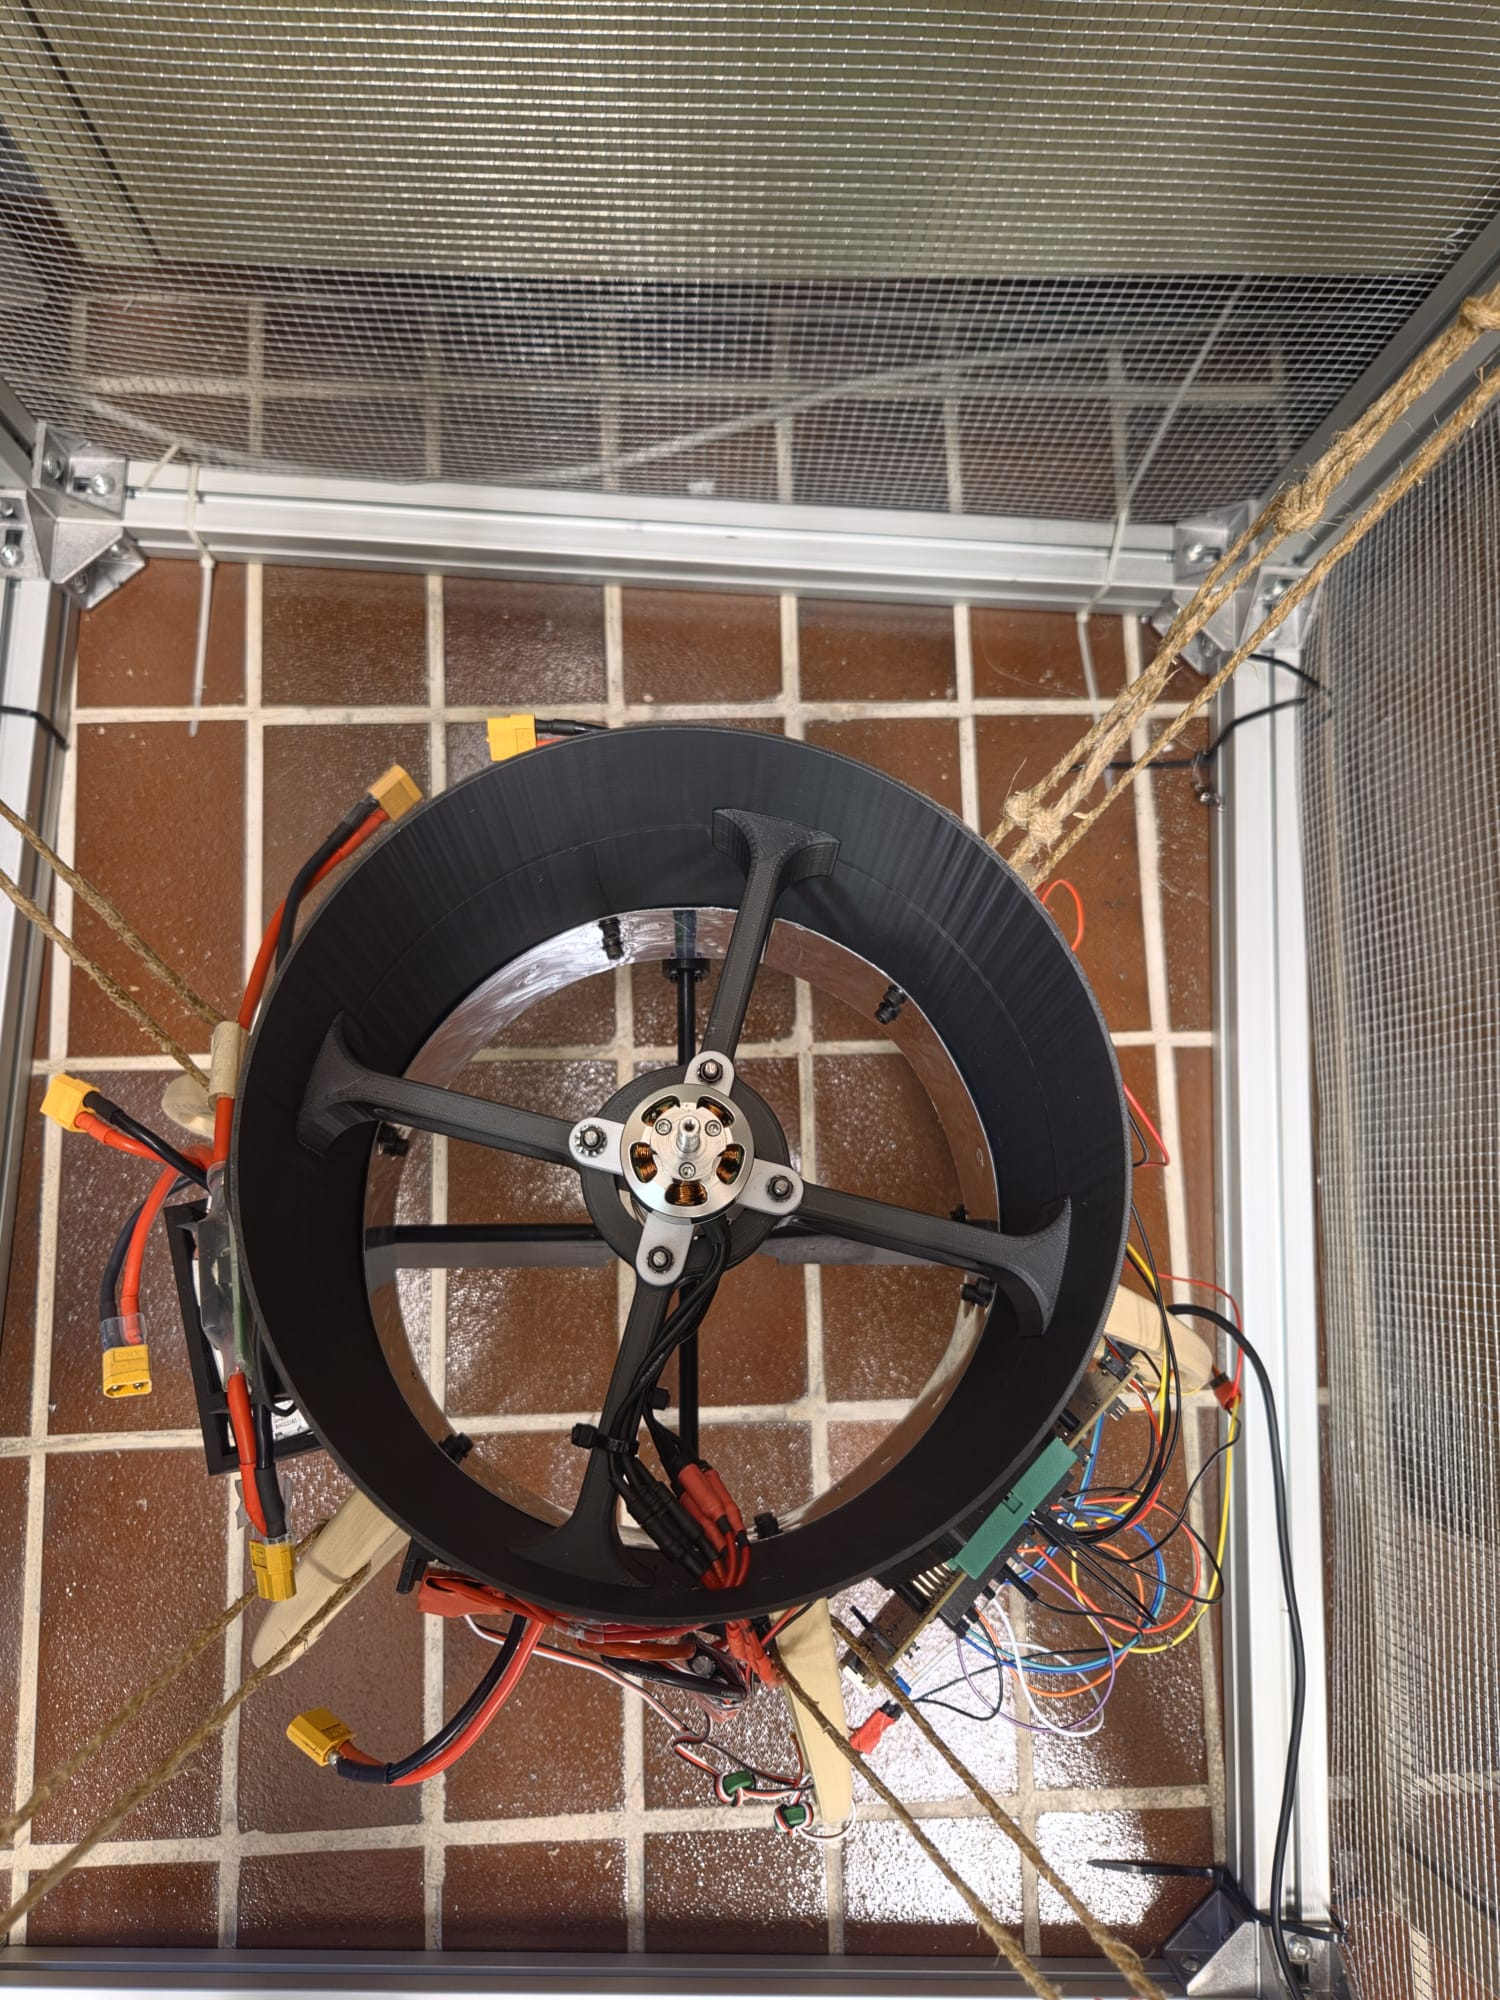
\includegraphics[height=5cm,keepaspectratio]{figures/01_sistema/struttura_ducted_fan_1.jpg}
			\caption{Struttura di sostegno dei motori}
		\end{subfigure}
		\hfill
		\begin{subfigure}[b]{0.48\textwidth}
			\centering
			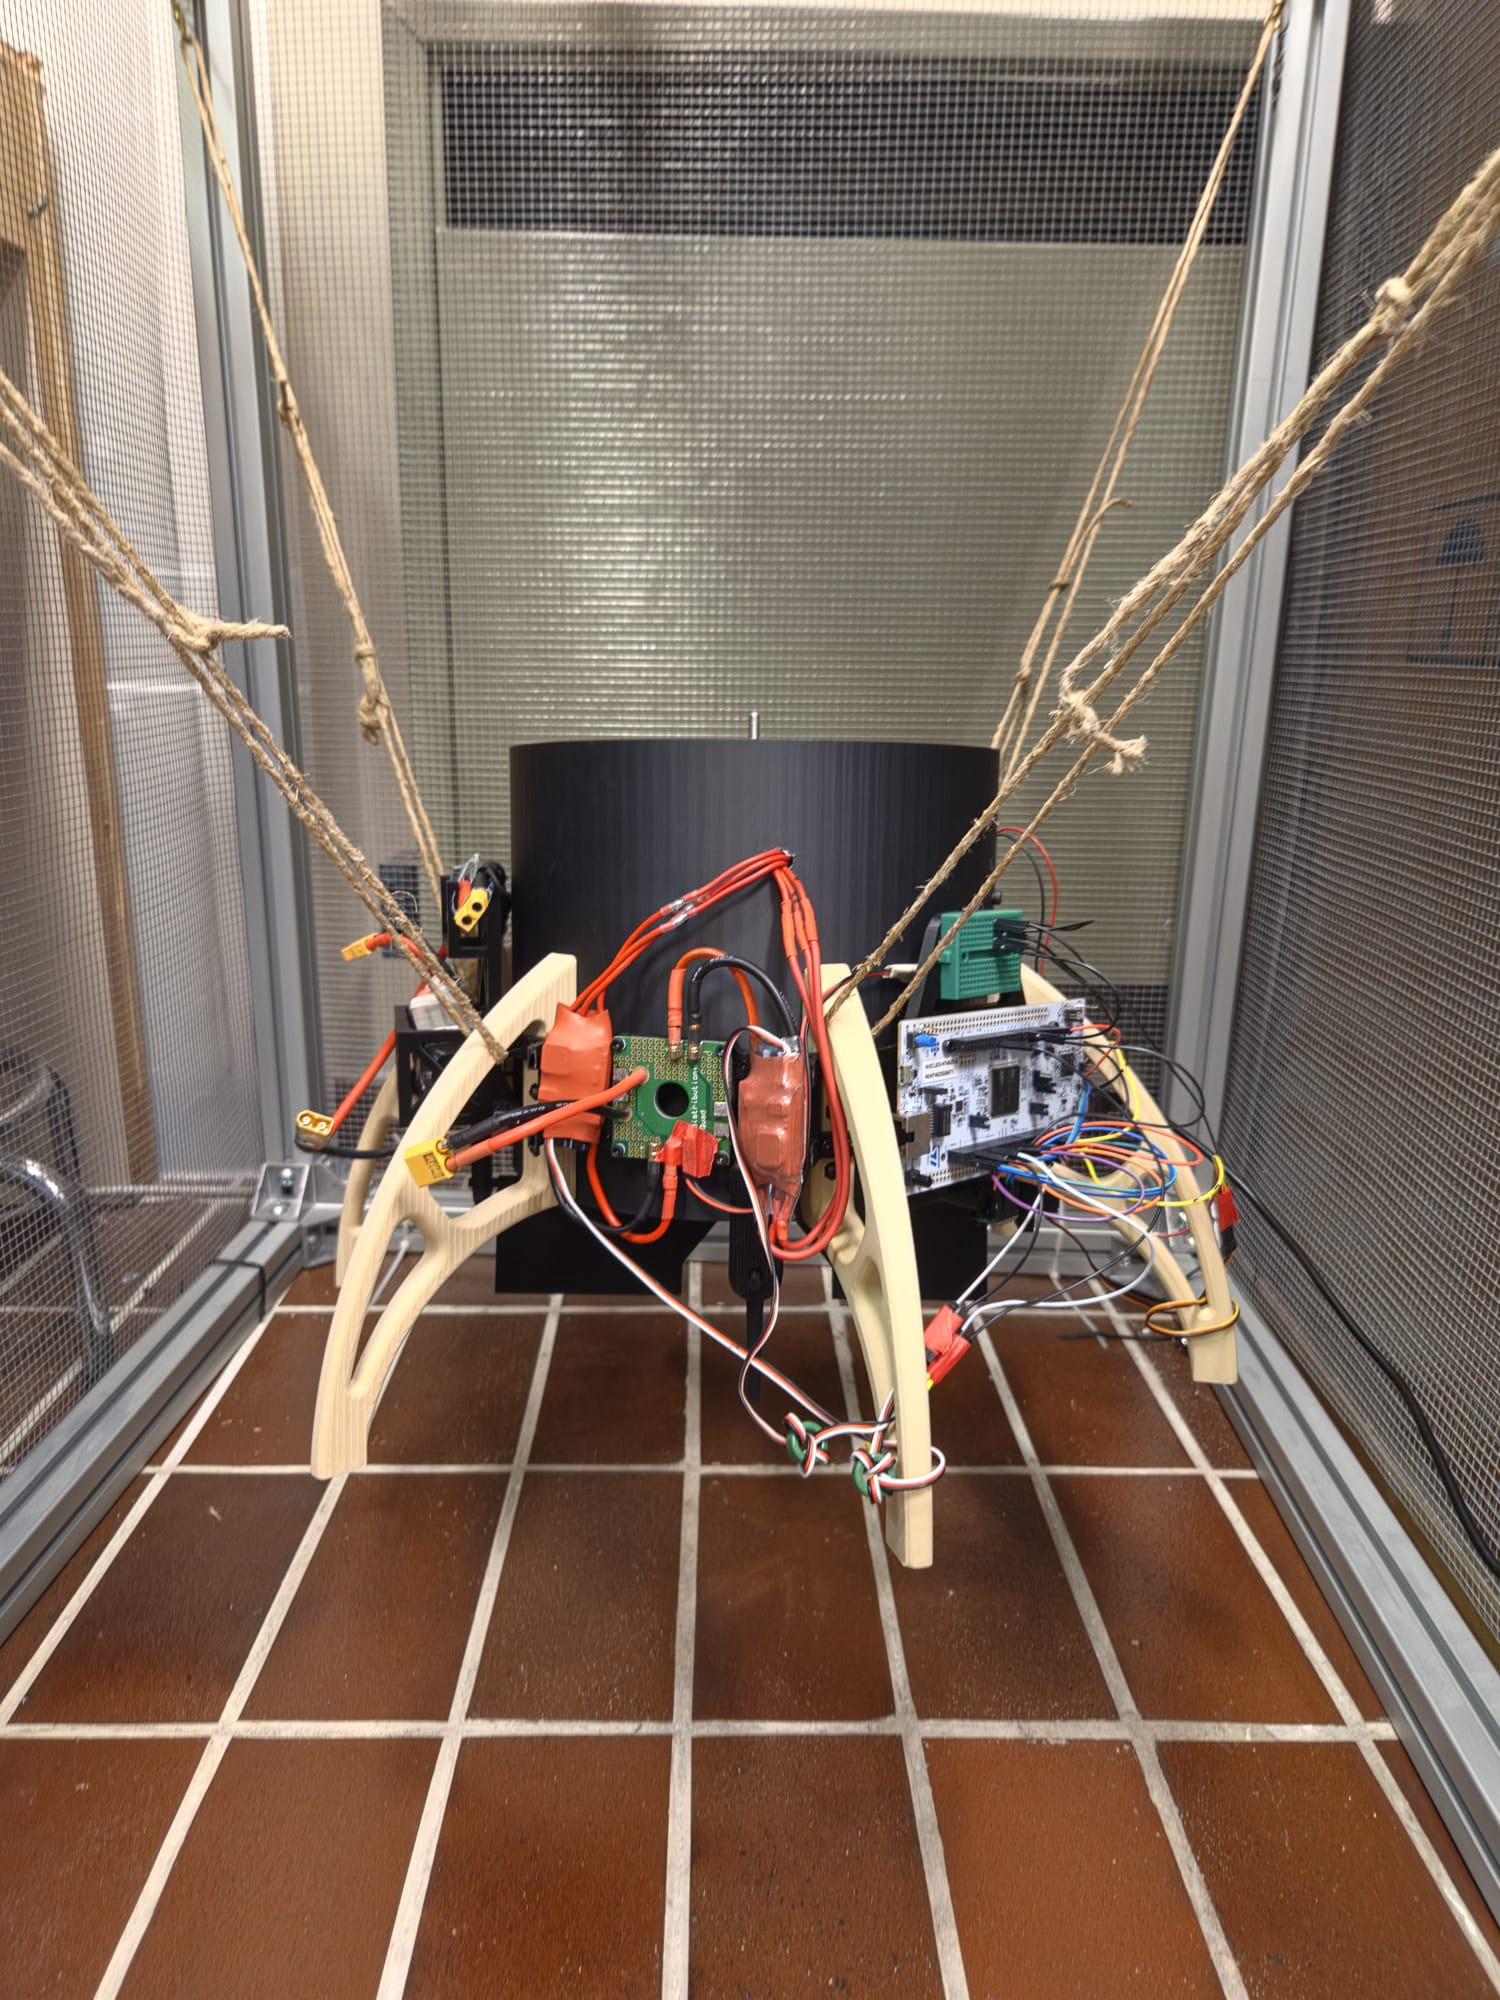
\includegraphics[height=5cm,keepaspectratio]{figures/01_sistema/struttura_ducted_fan_2.jpg}
			\caption{Vista frontale}
		\end{subfigure}
		\caption{Struttura del ducted fan}
		\label{fig:struttura_ducted_fan}
	\end{figure}
	
	Dal punto di vista teorico, l'adozione di rotori controrotanti permette di generare spinta verticale limitando al contempo la rotazione del drone attorno all'asse Z, grazie ai momenti torcenti opposti prodotti dalle eliche. Tuttavia, i test sperimentali hanno evidenziato che questa compensazione passiva, per quanto utile, non è sufficiente a stabilizzare in modo del tutto autonomo la dinamica di imbardata (\textit{yaw}), rendendo imprescindibile l'implementazione di un'azione di controllo dedicata.\\
	Un'ulteriore criticità legata al \textit{design} strutturale del \textit{DPDF} è la sua naturale suscettibilità a rotazioni indesiderate sul piano definito dagli assi X e Y. Tali perturbazioni rischiano di compromettere la stabilità del sistema, potendo causare una completa perdita di controllo del mezzo. Per limitare questo fenomeno, la parte inferiore del drone è stata equipaggiata con due \textbf{flap} direzionali: uno dedicato al controllo dell'assetto lungo l'asse delle ascisse e l'altro lungo l'asse delle ordinate, disposti in modo tale da risultare perpendicolari tra loro.\\
	Questi \textit{flap} agiscono come vere e proprie superfici aerodinamiche di controllo per la compensazione dei disturbi di rollio (\textit{roll}) e beccheggio (\textit{pitch}). Il principio di regolazione si basa sull'interazione tra i \textit{flap} e il flusso d'aria discendente generato dai motori: ruotando di un piccolo angolo, il \textit{flap} devia la traiettoria del getto d'aria che lo investe, alterando la distribuzione delle pressioni tra la faccia esposta al flusso (lato di pressione) e quella opposta (lato di depressione). Tale gradiente di pressione genera una forza aerodinamica risultante, approssimabile come perpendicolare alla superficie del \textit{flap} stesso, in grado di imprimere al velivolo un momento correttivo sull'assetto. Affinché il controllo sia efficace, la direzione e il verso di questa forza vengono gestiti in modo da contrastare esattamente il momento perturbativo iniziale. Dal punto di vista meccanico, ciascun \textit{flap} è vincolato a un'estremità al rispettivo servomotore di attuazione, mentre l'estremità opposta è inserita in un apposito modulo strutturale che ne garantisce il mantenimento del parallelismo rispetto al suolo.\\
	Per quanto riguarda l'elettronica di bordo, le componenti hardware necessarie al funzionamento del sistema (che saranno oggetto di un'analisi dettagliata nel Capitolo~\ref{ch:hardware}) sono state collocate lungo la superficie esterna del cilindro. La loro disposizione è stata studiata con l'obiettivo di ottenere il miglior bilanciamento possibile delle masse. Sempre all'esterno sono stati integrati sei piedi d'appoggio, disposti in corrispondenza dei vertici di un esagono regolare inscritto nella circonferenza di base del \textit{DPDF}, assicurando così un supporto a terra stabile e una ripartizione omogenea dei pesi.\\
	Infine, dal punto di vista realizzativo, l'intera struttura cilindrica, i \textit{flap}, i piedi di appoggio e i supporti per l'hardware e per i motori sono stati fabbricati tramite \textbf{stampa 3D}, impiegando il \textbf{PLA} come materiale principale. Le singole parti sono state stampate separatamente per poi essere assemblate e fissate tra loro, andando a costituire il telaio definitivo del sistema. Una panoramica visiva che illustra gli ingombri, la geometria generale della struttura esterna e il dettaglio dei sostegni dei motori è riportata in Figura~\ref{fig:render_dpdf}.
	
	\begin{figure}[H]
		\centering
		\begin{subfigure}[b]{0.48\textwidth}
			\centering
			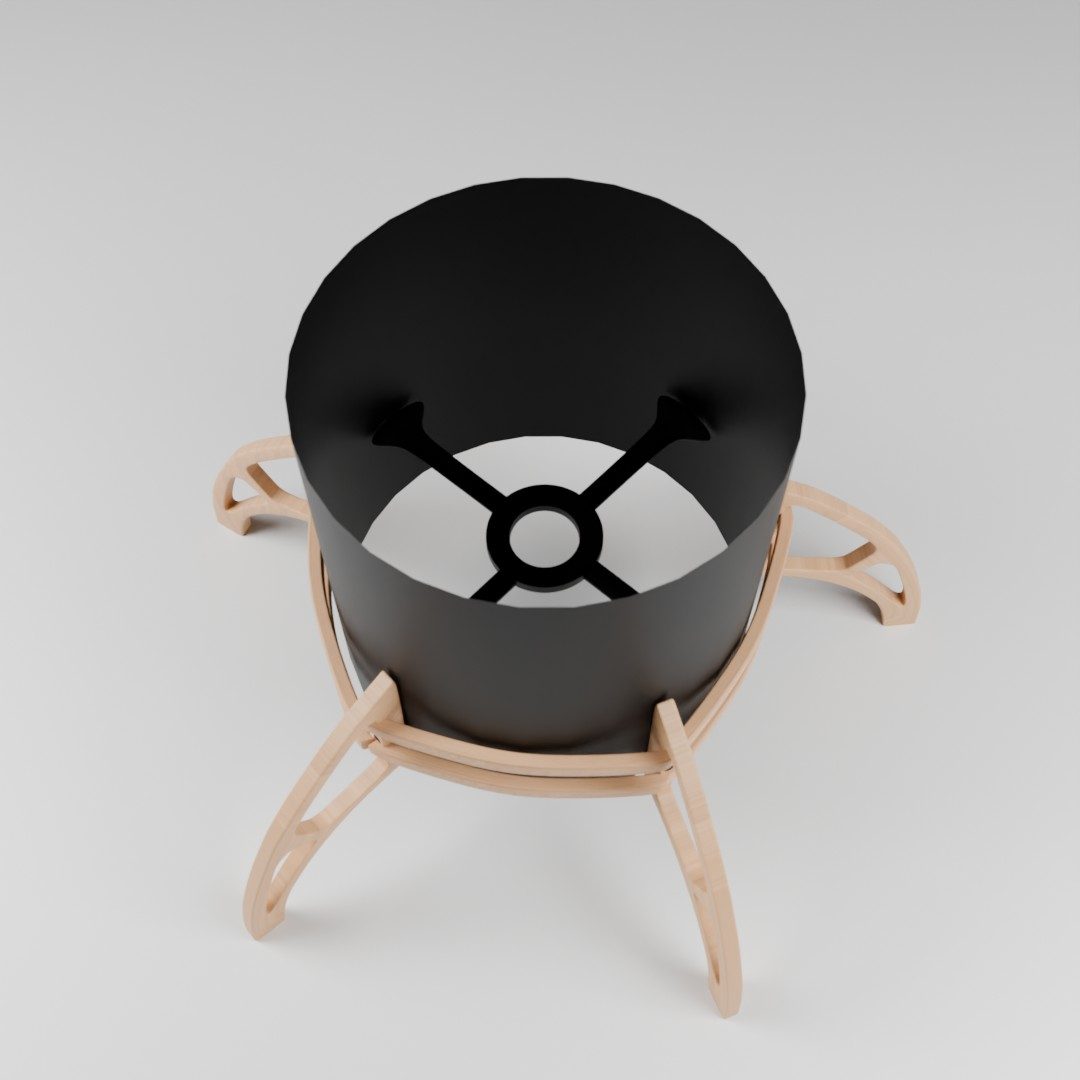
\includegraphics[height=5.5cm,keepaspectratio]{figures/01_sistema/render_dpdf_1.png}
		\end{subfigure}
		\hfill
		\begin{subfigure}[b]{0.48\textwidth}
			\centering
			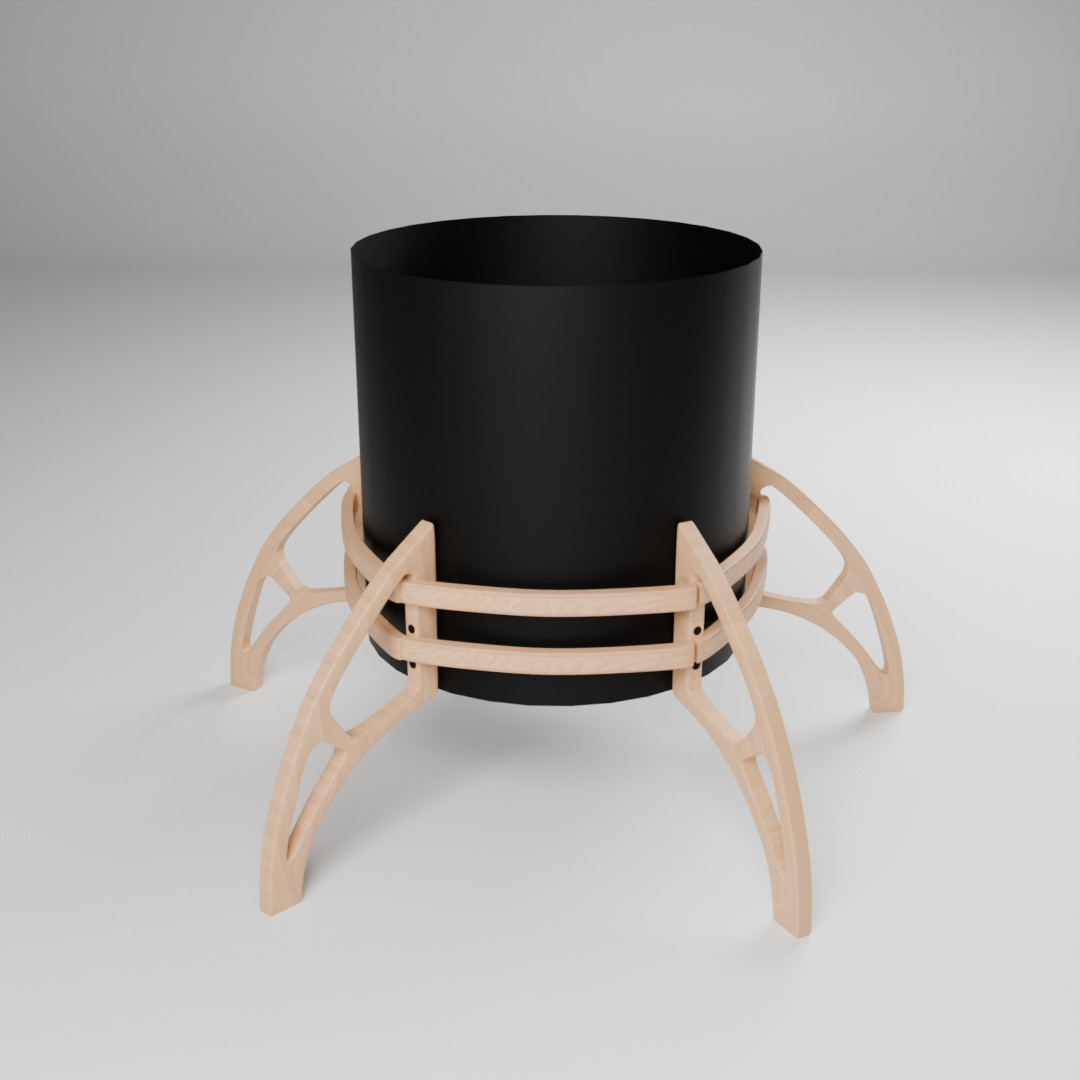
\includegraphics[height=5.5cm,keepaspectratio]{figures/01_sistema/render_dpdf_2.png}
		\end{subfigure}
		\caption{Render Ducted Fan}
		\label{fig:render_dpdf}
	\end{figure}
	
	\section{Controllo del Double Propeller Ducted-Fan}
	La configurazione del \textit{DPDF}, pur ottimizzata per l'efficienza del flusso d'aria, presenta complessità dinamiche dovute a tolleranze costruttive, asimmetrie tra i propulsori e flussi turbolenti interni al condotto. Tali fattori rendono difficoltosa una descrizione accurata tramite modelli lineari derivati analiticamente e rendono la taratura empirica dei regolatori un processo incerto e non riproducibile.\\
	Il presente lavoro risponde a questa sfida attraverso un approccio \textbf{data-driven} basato su tre livelli. Il primo livello è la costruzione di un'\textit{infrastruttura di telemetria} che trasforma il drone in una piattaforma capace di registrare ogni variabile di stato rilevante a 50 [Hz] e di ricevere in tempo reale segnali di eccitazione strutturati generati da MATLAB. Il secondo livello è l'\textit{identificazione di sistema}: i \textit{dataset} acquisiti durante prove di eccitazione PRBS vengono elaborati per stimare le funzioni di trasferimento $G_\text{roll}(z)$ e $G_\text{pitch}(z)$, che descrivono per ciascun asse il legame tra angolo imposto al \textit{flap} e risposta angolare del corpo. Il terzo livello è la \textit{simulazione}: un modello fisico 3D calibrato sui dati reali permette di verificare il comportamento dei regolatori sintetizzati in un ambiente sicuro, prima della validazione sul sistema fisico.\\
	L'insieme di questi tre livelli costituisce la pipeline completa del progetto e la struttura attorno alla quale è organizzato il presente documento, descritta nei Capitoli~3--6.
	\newpage
	
	%%%%%%%%%%%%%%%%%%%%%%%%%%%%%%%%%%%%%%%%%%%%%%%%%%%%%%%%%%%%%%%%%%%%
	%                         CAPITOLO 2 - HARDWARE
	%%%%%%%%%%%%%%%%%%%%%%%%%%%%%%%%%%%%%%%%%%%%%%%%%%%%%%%%%%%%%%%%%%%%
	\chapter{Hardware}
	\label{ch:hardware}
	Nel presente capitolo vengono descritte le componenti hardware impiegate nel progetto per la realizzazione e il controllo del \textit{DPDF}. Per ciascun elemento verranno illustrati il ruolo specifico all'interno del sistema, le principali specifiche fisiche e tecniche, nonché le rispettive modalità di utilizzo e interfacciamento. A conclusione dell'analisi, verrà presentato un diagramma esplicativo accompagnato da una tabella riepilogativa, al fine di chiarire l'architettura complessiva dei collegamenti elettrici e logici.
	
	%--------------------------------------------------------------
	\section{STM32 NUCLEO-H745ZI-Q. La scheda di controllo}
	La scheda \textit{STM32 NUCLEO-H745ZI-Q} \cite{stm32_nucleo_um} è una piattaforma di sviluppo avanzata prodotta da \textit{STMicroelectronics}. Il cuore del sistema è il microcontrollore \textit{STM32H745ZI-TQ6}, appartenente alla famiglia \textit{STM32H7} ad alte prestazioni. Questo dispositivo è stato concepito per agevolare lo sviluppo, il \textit{debug} e la prototipazione rapida di applicazioni \textit{embedded} di elevata complessità. All'interno del progetto, la \textit{NUCLEO-H745ZI-Q} ha assolto il ruolo di unità di calcolo centrale per lo sviluppo e il collaudo del firmware di gestione di tutte le periferiche e delle logiche di volo del \textit{DPDF}. L'implementazione e il caricamento delle librerie software dedicate sono stati eseguiti avvalendosi dell'ambiente di sviluppo integrato \textit{STM32CubeIDE}. Di seguito viene fornita una descrizione dettagliata delle principali caratteristiche del microcontrollore \textit{STM32H745ZI-TQ6}, la cui architettura generale è illustrata in Figura~\ref{fig:stm32h745zi_chip}.
	
	\begin{figure}[H]
		\centering
		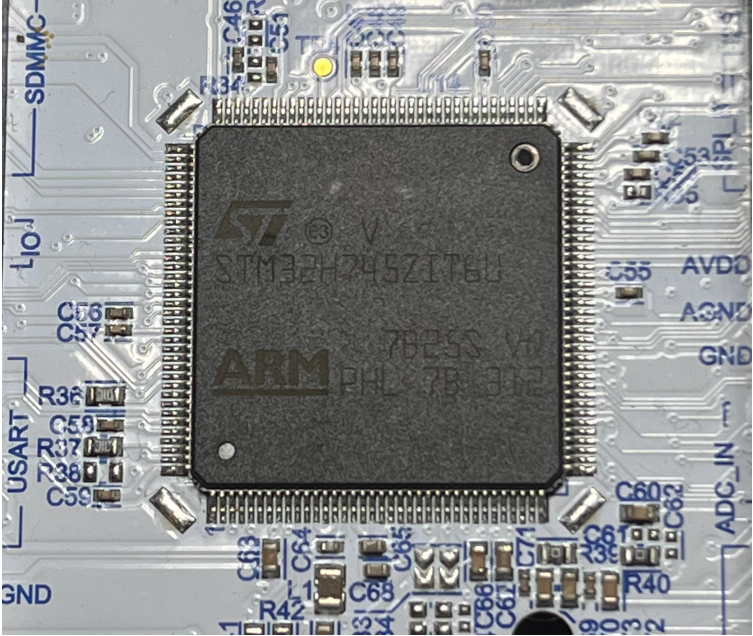
\includegraphics[width=0.55\textwidth]{figures/02_hardware/stm32h745zi_chip.png}
		\caption{Il microcontrollore STM32H745ZI-TQ6}
		\label{fig:stm32h745zi_chip}
	\end{figure}
	
	\subsection{STM32H745ZI-TQ6. Architettura}
	Il microcontrollore \textit{STM32H745ZI-TQ6} si distingue per un'architettura \textit{dual-core} a 32-bit. Essa integra un processore primario ad altissime prestazioni, l'\textit{Arm Cortex-M7} (capace di operare a una frequenza massima di \textbf{480 MHz}), affiancato da un coprocessore \textit{Arm Cortex-M4} (con frequenza massima di \textbf{240 MHz}). Per le specifiche esigenze di questo progetto, l'esecuzione del firmware e la gestione delle librerie relative ai sensori e agli attuatori sono state interamente demandate al core \textit{Cortex-M4}. Sebbene l'hardware supporti frequenze operative nettamente superiori, in fase di dimensionamento si è scelto di impostare la frequenza di clock effettiva a \textbf{75 MHz}. Tale configurazione è stata generata e definita mediante l'interfaccia grafica \textit{Clock Configuration} fornita dal file di progetto \texttt{.ioc}.
	
	\subsection{STM32H745ZI-TQ6. Timer}
	Per quanto riguarda il comparto delle temporizzazioni, il microcontrollore mette a disposizione \textbf{15 timer} ad alta risoluzione e \textbf{5 \textit{Low-Power Timer}}. Questi moduli risultano fondamentali per la misurazione del tempo, la schedulazione di eventi periodici e, soprattutto, per la generazione dei segnali PWM (\textit{Pulse-Width Modulation}) necessari al controllo della catena cinematica. Nello specifico, il firmware sviluppato sfrutta i seguenti moduli:
	\begin{itemize}
		\item \textbf{TIM2}: deputato alla generazione dei segnali PWM per il controllo di posizione dei servomotori dei \textit{flap}.
		\item \textbf{TIM4}: impiegato per la generazione dei segnali PWM destinati agli ESC (\textit{Electronic Speed Controllers}) per la regolazione del regime di rotazione dei motori principali.
		\item \textbf{TIM6}: configurato per gestire la sequenza temporizzata di \textit{safe startup} (avvio in sicurezza) e per il pilotaggio diagnostico dei LED integrati sulla scheda.
		\item \textbf{TIM7}: utilizzato come \textit{timebase} per la generazione periodica dell'\textit{interrupt} che innesca l'aggiornamento del ramo di controllo IMU-servomotori, seguendo un paradigma di tipo \textit{event-driven}.
	\end{itemize}
	
	\subsection{STM32H745ZI-TQ6. Periferiche di comunicazione}
	Il microcontrollore integra un vasto set di periferiche di comunicazione. Ai fini dell'interfacciamento hardware richiesto dal \textit{DPDF}, assumono particolare rilevanza i protocolli di comunicazione seriale sincrona e asincrona, tra cui $I^{2}C$, \textit{USART/UART} e \textit{SPI}. Tali interfacce sono state impiegate per stabilire il collegamento dati tra l'unità di controllo, i sensori di assetto/quota e gli strumenti di sviluppo e telemetria. Il chip offre inoltre il supporto nativo per bus di comunicazione di livello superiore, quali \textit{CAN}, \textit{USB OTG} ed \textit{Ethernet}, sebbene questi ultimi non siano stati impiegati nell'attuale implementazione del sistema.
	
	\subsection{STM32H745ZI-TQ6. Eventi asincroni}
	La gestione degli eventi asincroni e delle interruzioni hardware è orchestrata dal modulo \textbf{NVIC} (\textit{Nested Vectored Interrupt Controller}). Questo componente hardware consente di trattare in modo deterministico ed estremamente efficiente le routine di servizio delle interruzioni (\textit{ISR}), garantendo una corretta gerarchia di priorità \textit{pre-emptive}. L'efficienza del \textit{NVIC} rappresenta un requisito cruciale per garantire la stabilità temporale e l'affidabilità dell'architettura \textit{event-driven} alla base del firmware di controllo del volo.
	
	\subsection{NUCLEO-H745ZI-Q. Caratteristiche della scheda}
	
	\paragraph{Caratteristiche fisiche}\mbox{}\\
	\begin{itemize}
		\item Dimensioni: $133.34\times 70.00$ [mm].
		\item Peso: 120 [g].
	\end{itemize}
	
	\paragraph{Programmazione e Debug (ST-LINK/V3E)}\mbox{}\\
	La scheda integra il modulo \textit{ST-LINK/V3E}, il quale consente la programmazione e il \textit{debug} del firmware direttamente tramite connessione USB. Tale modulo fornisce inoltre due interfacce ausiliarie di fondamentale utilità durante le fasi di sviluppo:
	\begin{itemize}
		\item \textbf{VCP (Virtual COM Port)}: emula una porta seriale su interfaccia USB, agevolando lo scambio di dati e la telemetria.
		\item \textbf{MSC (Mass Storage Class)}: espone la scheda al sistema operativo host come una memoria di massa esterna, semplificando le operazioni di caricamento dei file binari.
	\end{itemize}
	
	\paragraph{Gestione dell'alimentazione}\mbox{}\\
	La piattaforma garantisce un'elevata flessibilità per quanto concerne l'alimentazione, ammettendo tre configurazioni principali:
	\begin{itemize}
		\item Alimentazione a 5 V fornita tramite la porta USB Micro-B dell'interfaccia ST-LINK.
		\item Alimentazione esterna compresa tra 7 V e 12 V mediante l'apposito Jack esterno.
		\item Alimentazione diretta a 3.3 V tramite il pin \textit{Vin} esterno.
	\end{itemize}
	Indipendentemente dalla sorgente primaria adottata, il microcontrollore è stabilizzato per operare a 3.3 V per mezzo di regolatori di tensione interni. La selezione della modalità di alimentazione avviene attraverso l'impostazione meccanica di specifici \textit{bridge} (\textit{jumper}) che cortocircuitano determinate coppie di pin. Di conseguenza, qualora si opti per sorgenti diverse dalla connessione USB standard (\textit{ST-LINK}), è indispensabile verificare preventivamente e con attenzione la corretta configurazione di tali ponticelli. Il dettaglio dei \textit{bridge} rilevanti per l'alimentazione è illustrato in Figura~\ref{fig:nucleo_bridge}.
	
	\begin{figure}[H]
		\centering
		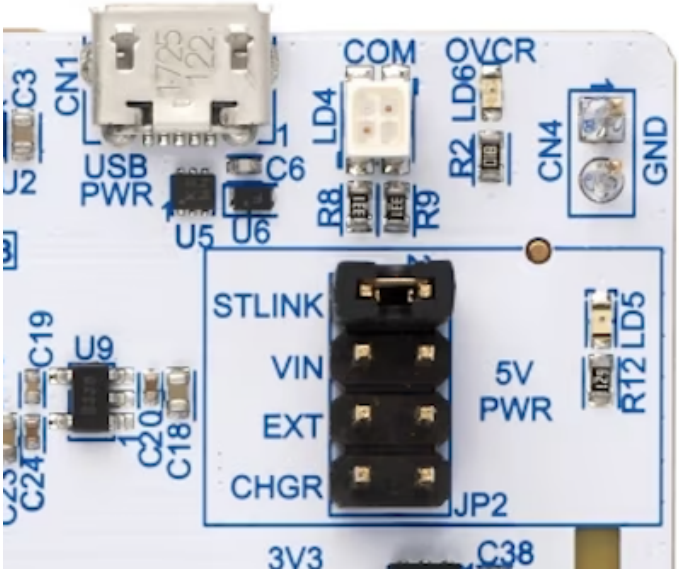
\includegraphics[width=0.5\textwidth]{figures/02_hardware/nucleo_bridge_alimentazione.png}
		\caption{NUCLEO-H745ZI-Q. Dettaglio esplicativo dei bridge}
		\label{fig:nucleo_bridge}
	\end{figure}
	
	\paragraph{Formato fisico ed espandibilità}\mbox{}\\
	Appartenendo alla linea \textit{Nucleo-144} di \textit{STMicroelectronics}, la scheda di sviluppo mette a disposizione due connettori di tipo \textit{Morpho}, i quali espongono e rendono liberamente accessibili tutti i 144 pin del microcontrollore. Questo sistema di espansione proprietario prende il nome di \textit{ST Zio}. A ulteriore supporto della prototipazione, la \textit{NUCLEO-H745ZI-Q} garantisce la piena compatibilità hardware e di piedinatura (\textit{pinout}) per l'alloggiamento degli \textit{shield} standardizzati per Arduino Uno R3. Una vista complessiva della scheda e delle sue interfacce è riportata in Figura~\ref{fig:nucleo_board}.
	
	\begin{figure}[H]
		\centering
		\begin{subfigure}[b]{0.48\textwidth}
			\centering
			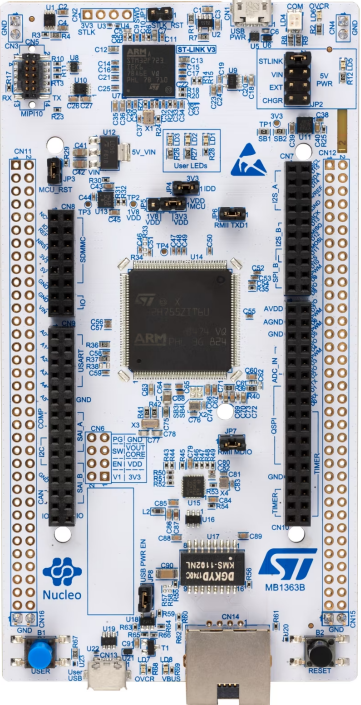
\includegraphics[height=5cm,keepaspectratio]{figures/02_hardware/nucleo_h745zi_q_fronte.png}
			\caption{Vista frontale}
		\end{subfigure}
		\hfill
		\begin{subfigure}[b]{0.48\textwidth}
			\centering
			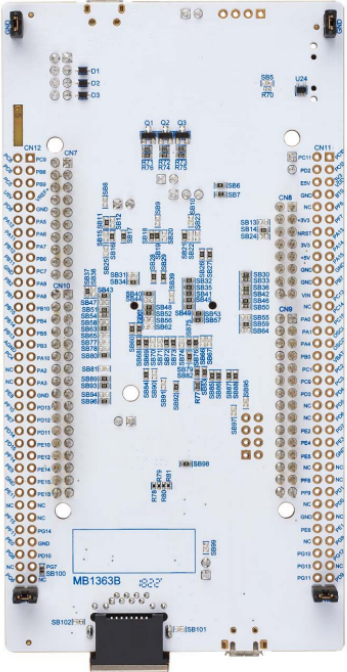
\includegraphics[height=5cm,keepaspectratio]{figures/02_hardware/nucleo_h745zi_q_retro.png}
			\caption{Vista posteriore}
		\end{subfigure}
		\caption{La scheda di sviluppo NUCLEO-H745ZI-Q}
		\label{fig:nucleo_board}
	\end{figure}
	
	%--------------------------------------------------------------
	\section{TATTU LiPo. Batteria ricaricabile}
	Motori, servomotori ed ESC richiedono specifici livelli di tensione per il loro funzionamento, tensioni che non possono essere fornite dalla \textit{NUCLEO H745ZI-Q}. Si rende, quindi, necessario l'inserimento nel progetto di batterie ricaricabili. In base alle prestazioni richieste dal progetto, si è optato per le \textbf{TATTU LiPo}.
	
	\subsection{TATTU LiPo. Caratteristiche fisiche}
	\begin{itemize}
		\item Dimensioni: $74\times 35.5\times 29$ [mm].
		\item Peso: 150 [g].
		\item Numero di celle: 4.
	\end{itemize}
	
	\subsection{TATTU LiPo. Caratteristiche tecniche e considerazioni operative}
	
	\paragraph{Tensione}\mbox{}\\
	L'accumulatore adottato per l'alimentazione del sistema è una batteria \textit{TATTU LiPo} (\textit{Litio-Polimero}) configurata in architettura \textbf{4S}, ossia composta da 4 celle collegate in serie. Essendo la tensione nominale di ogni singola cella pari a \textbf{3.7 [V]}, il pacco batteria fornisce una tensione nominale complessiva di \textbf{14.8 [V]}. In condizioni di carica completa, la tensione per singola cella raggiunge i \textbf{4.2 [V]}, portando la tensione totale a \textbf{16.8 [V]}. Al fine di preservare la vita utile dell'accumulatore e rallentarne il degrado chimico, è fondamentale mantenere la tensione il più possibile prossima al valore nominale, evitando periodi prolungati di permanenza in stato di carica massima e, soprattutto, fenomeni di scarica profonda. A tale scopo, è strettamente necessario evitare che la tensione complessiva scenda al di sotto dei \textbf{12.8 [V]}, garantendo in questo modo che la tensione di ciascuna cella non si riduca mai oltre la soglia critica di \textbf{3.2 [V]}.
	
	\paragraph{Capacità}\mbox{}\\
	La capacità, misurata in [mAh], indica la quantità di carica elettrica che la batteria è in grado di immagazzinare e successivamente erogare nel tempo. Nel caso in esame, la capacità nominale della singola \textit{LiPo} è pari a \textbf{1300 [mAh]}, il che significa che l'accumulatore è teoricamente in grado di erogare una corrente continua di 1.3 [A] per la durata di un'ora. In prima approssimazione, l'autonomia temporale del sistema può essere stimata attraverso la seguente relazione:
	\begin{equation}
		t_h = \frac{C\,[\textrm{mAh}]}{A\,[\textrm{mA}]}
		\label{eq:autonomia_batteria}
	\end{equation}
	dove $t_h$ rappresenta il tempo di funzionamento stimato (espresso in ore), $C$ è la capacità della batteria in [mAh] e $A$ è la corrente media assorbita dal carico, espressa in [mA].\\
	Al fine di incrementare l'autonomia di volo, nel presente progetto si è optato per il collegamento in \textbf{parallelo} di due unità \textit{TATTU LiPo} identiche, raddoppiando di fatto la capacità totale a disposizione fino a \textbf{2600 [mAh]}. Tale parallelo è stato realizzato in sicurezza impiegando il modulo \textit{PowerSafe Twin}, prodotto da \textit{MNR-electronics}, le cui caratteristiche verranno approfondite nella sezione successiva.
	
	\paragraph{Capacità di scarica (C-rating)}\mbox{}\\
	La capacità di scarica definisce la corrente massima che l'accumulatore può erogare in modo continuativo senza subire danni strutturali o surriscaldamenti. Le batterie \textit{TATTU LiPo} impiegate presentano un rateo di scarica nominale pari a \textbf{75C}. Di conseguenza, la corrente massima teorica erogabile dalla singola batteria è calcolabile come segue:
	\begin{equation}
		A_{max} = C_s \cdot C \quad \Rightarrow \quad A_{max} = 75\,[\textrm{C}] \cdot 1.3\,[\textrm{A}] = 97.5\,[\textrm{A}]
		\label{eq:c_rating}
	\end{equation}
	dove $A_{max}$ è la corrente massima continua espressa in [A], $C_s$ è il rateo di scarica caratteristico e $C$ indica la capacità nominale dell'accumulatore (convertita in Ampere-ora). Una rappresentazione visiva del pacco batteria assemblato e impiegato durante le sessioni di prova è fornita in Figura~\ref{fig:tattu_lipo}.
	
	\begin{figure}[H]
		\centering
		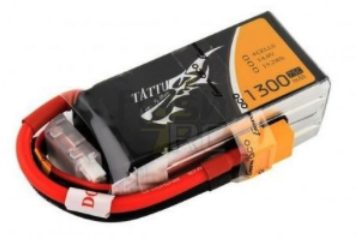
\includegraphics[width=0.45\textwidth]{figures/02_hardware/tattu_lipo.jpg}
		\caption{TATTU LiPo 4S 1300mAh 75C}
		\label{fig:tattu_lipo}
	\end{figure}
	
	%--------------------------------------------------------------
	\section{PowerSafe Twin ADV. MNR-electronics}
	Al fine di garantire la massima sicurezza e affidabilità del sistema di alimentazione a doppio pacco batteria, è stato integrato un modulo di ridondanza attiva: il \textbf{PowerSafe Twin ADV}, prodotto da \textit{MNR-electronics}.\\
	Questo dispositivo rappresenta una soluzione avanzata per la gestione sicura dell'energia di bordo. Il modulo, infatti, effettua un monitoraggio continuo delle principali variabili di stato (quali tensione e corrente), selezionando in tempo reale l'accumulatore ottimale per l'alimentazione del carico. Qualora, ad esempio, la tensione di una batteria dovesse scendere al di sotto di una soglia critica di sicurezza, il sistema commuterebbe in modo del tutto automatico sull'unità secondaria, scongiurando così qualsiasi interruzione transitoria o calo significativo nell'erogazione di potenza ai motori e all'elettronica.\\
	Analizzando l'architettura interna del sistema, è possibile distinguere tre sezioni funzionali principali:
	\begin{itemize}
		\item \textbf{Modulo di potenza}: è preposto alla gestione della commutazione hardware tra i pacchi batteria, al bilanciamento e alla distribuzione della corrente verso il carico. Questa sezione integra inoltre i circuiti di protezione necessari per isolare il sistema in caso di guasto elettrico (es. cortocircuito o sovracorrente).
		\item \textbf{Modulo di controllo}: basato su un microprocessore dedicato, ha il compito di campionare e analizzare costantemente le grandezze elettriche (come i livelli di tensione, gli assorbimenti di corrente e i potenziali squilibri tra le celle), implementando fisicamente la logica algoritmica che governa la ridondanza attiva.
		\item \textbf{Modulo di allarme}: fornisce un \textit{feedback} diagnostico all'operatore, segnalando l'insorgenza di eventuali anomalie operative o cali di tensione critici attraverso indicatori luminosi (LED) e avvisi acustici.
	\end{itemize}
	Una raffigurazione del dispositivo impiegato per l'assemblaggio del \textit{DPDF} è riportata in Figura~\ref{fig:powersafe_twin}.
	
	\begin{figure}[H]
		\centering
		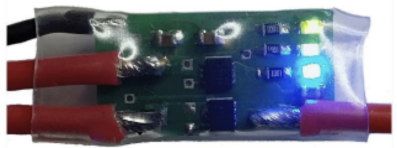
\includegraphics[width=0.45\textwidth]{figures/02_hardware/powersafe_twin.jpg}
		\caption{PowerSafe Twin ADV MNR-electronics}
		\label{fig:powersafe_twin}
	\end{figure}
	
	\subsection{PowerSafe Twin ADV. Caratteristiche fisiche e tecniche}
	\begin{itemize}
		\item Dimensioni con involucro protettivo: $80\times 59\times 26$ [mm].
		\item Peso, considerando sia l'involucro protettivo che i cablaggi (connettori XT60): 100 [g].
		\item Corrente massima gestibile: 100 [A] (in continua).
		\item Numero di celle per pacco batteria gestibili: $[3S \div 8S]$.
		\item Tensione massima ammessa in ingresso: $\approx 33.6$ [V]. Considerando il minimo 3.7 [V] e il massimo 4.2 [V] per cella: $[11.1 \div 33.6]$ [V].
	\end{itemize}
	
	%--------------------------------------------------------------
	\section{DFRobot Power Module. Convertitore di tensione}
	Al fine di garantire una corretta e sicura distribuzione dell'energia elettrica a tutte le periferiche di bordo, si è reso necessario l'impiego di moduli convertitori di tensione (\textit{DC-DC converter}), in grado di adattare la potenza erogata dalle batterie alle specifiche esigenze di ciascun dispositivo.\\
	Il componente selezionato per questo scopo è il \textit{DFRobot Power Module} \cite{dfrobot_pm}. Il dispositivo riceve in ingresso la tensione non regolata proveniente dal pacco batterie e la ripartisce, mettendo a disposizione differenti opzioni di alimentazione a seconda del terminale di uscita impiegato:
	\begin{itemize}
		\item \textbf{Uscita diretta (Pass-through)}: una prima soluzione progettuale fornita dal dispositivo consiste nell'erogare in uscita il medesimo valore di tensione applicato in ingresso. In questa configurazione, il modulo opera di fatto come un ponte elettrico per il trasferimento diretto della potenza.
		\item \textbf{Uscita stabilizzata a 5 [V]}: utilizzando dei pin dedicati presenti sulla scheda, il dispositivo è in grado di erogare una tensione regolata a 5 [V], selezionabile e attivabile mediante un apposito interruttore (\textit{switch}) hardware.
		\item \textbf{Uscita variabile}: infine, il modulo presenta un terminale la cui tensione di uscita è regolabile. Grazie alla presenza di un potenziometro (o \textit{trimmer}), è possibile tarare finemente la tensione desiderata su valori intermedi, fino a un massimo coincidente con la tensione di ingresso.
	\end{itemize}
	A causa degli elevati assorbimenti di corrente e per garantire la massima affidabilità del sistema di attuazione aerodinamica, la presenza dei due servomotori ha richiesto l'integrazione di \textbf{due convertitori di tensione distinti} all'interno dell'architettura hardware.\\
	Lo schema esplicativo che illustra la disposizione dei terminali di uscita è richiamato in Figura~\ref{fig:dfrobot_terminali}, mentre una fotografia del modulo convertitore effettivamente impiegato sul prototipo è riportata in Figura~\ref{fig:dfrobot_modulo}.
	
	\begin{figure}[H]
		\centering
		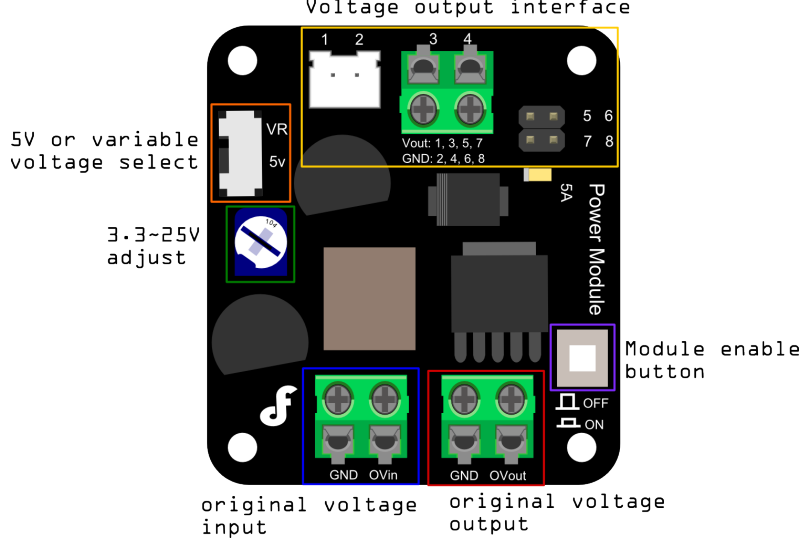
\includegraphics[width=0.6\textwidth]{figures/02_hardware/dfrobot_terminali.png}
		\caption{DFRobot Power Module. Disposizione dei terminali di uscita}
		\label{fig:dfrobot_terminali}
	\end{figure}
	
	\paragraph{Caratteristiche fisiche}\mbox{}\\
	\begin{itemize}
		\item Dimensioni: $46\times 50\times 20$ [mm].
		\item Peso: 35 [g].
	\end{itemize}
	
	\paragraph{Caratteristiche tecniche}\mbox{}\\
	\begin{itemize}
		\item Intervallo di tensione in ingresso: $[3.6 \div 25]$ [V].
		\item Intervallo di tensione esprimibile in uscita: $[3.3 \div 25]$ [V].
		\item Massima potenza erogabile: 25 [W].
		\item Frequenza di variazione: 350 [kHz].
	\end{itemize}
	
	\begin{figure}[H]
		\centering
		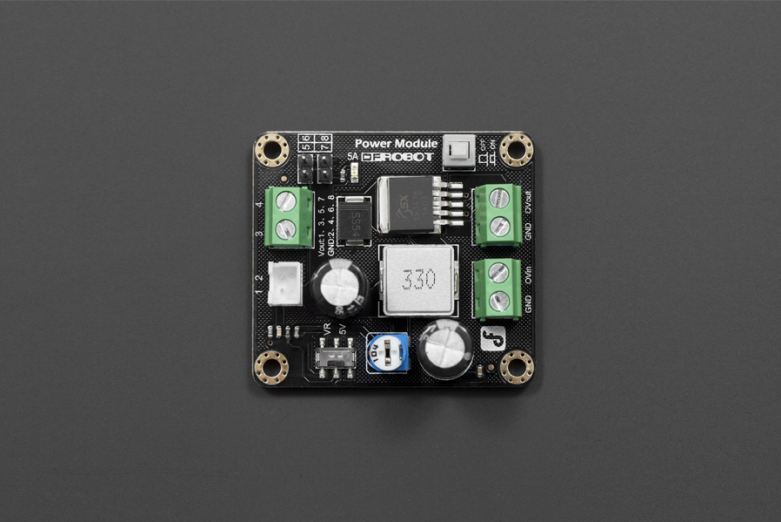
\includegraphics[width=0.45\textwidth]{figures/02_hardware/dfrobot_modulo.jpg}
		\caption{DFRobot Power Module}
		\label{fig:dfrobot_modulo}
	\end{figure}
	
	%--------------------------------------------------------------
	\section{Power Distribution Board}
	Con \textit{Power Distribution Board (PDB)} si fa riferimento ad un sottosistema elettrico la cui principale funzione è la \textbf{distribuzione in modo sicuro ed efficiente dell'energia fornita dal pacco batterie agli ESC} e, conseguentemente, ai motori. Ai fini progettuali, è stata selezionata una PDB, il cui punto di prelievo del segnale presenta un connettore \textbf{XT60}, adatto al pacco batterie. Il dispositivo integrato nel contesto operativo possiede inoltre quattro uscite, ciascuna in grado di erogare al massimo una corrente di \textbf{20 [A]}, e ha un peso complessivo di \textbf{27.3 [g]}. Una vista del componente è riportata in Figura~\ref{fig:pdb}.
	
	\begin{figure}[H]
		\centering
		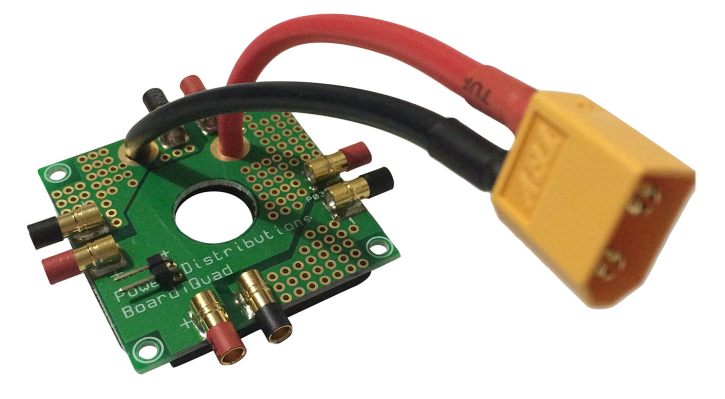
\includegraphics[width=0.45\textwidth]{figures/02_hardware/power_distribution_board.jpg}
		\caption{Power Distribution Board}
		\label{fig:pdb}
	\end{figure}
	
	%--------------------------------------------------------------
	\section{Turnigy AereoDrive SK3-3536 1400KV}
	Il \textbf{Turnigy AereoDrive SK3 3536 1400KV} è un motore \textit{brushless} trifase a magneti permanenti, il cui funzionamento richiede un \textit{Electronic Speed Controller (ESC)} per la corretta commutazione delle fasi. Invertendo due delle tre fasi è possibile invertire anche il senso di rotazione del motore. Nel progetto sono stati impiegati due motori di questo tipo in configurazione controrotante, così da ridurre le coppie di reazione delle eliche e contenere le rotazioni indesiderate di \textit{yaw}, senza però riuscire a compensarle completamente. Tale scelta è stata inoltre necessaria per garantire la spinta richiesta al sollevamento del sistema.
	
	\subsection{Turnigy AereoDrive SK3-3536 1400 KV. Caratteristiche fisiche e tecniche}
	\begin{itemize}
		\item Tensione operativa: $[11.1 \div 16.8]$ [V].
		\item Valore KV: 1400 RPM/V.
		\item Potenza massima: 590 [W].
		\item Corrente massima: 40 [A].
		\item Resistenza interna: $[0.021 \div 0.025]$ [$\Omega$].
		\item Corrente a vuoto: 0.021 [A].
		\item Diametro dell'albero motore: 5 [mm].
		\item Peso: 111 [g].
		\item Spaziatura fori di montaggio: $25\times 25$ [mm].
		\item Connettori \textit{bullet} da 3.5 [mm].
		\item Numero dei poli: 12.
	\end{itemize}
	Il valore "KV" indica il numero di giri al minuto (RPM) che il motore compie per ogni volt applicato a vuoto, in formula:
	\begin{equation}
		RPM = KV \cdot V
		\label{eq:kv_motor}
	\end{equation}
	A tensioni di alimentazione maggiori rispetto a quelle specificate il motore rischia di assorbire troppa corrente e surriscaldarsi. I giri al minuto massimi dipenderanno dalla tensione applicata e dalle dimensioni delle eliche. Nel presente progetto, il motore in interesse deve essere alimentato a batteria, vale a dire in corrente continua, lasciando spazio alla necessità di un dispositivo che trasformi la tensione continua erogata dalle batterie in un segnale trifase a corrente alternata. Il dispositivo in questione è il precedentemente citato \textit{Electronic Speed Controller}. Il motore adottato nel progetto è mostrato in Figura~\ref{fig:turnigy_motor}.
	
	\begin{figure}[H]
		\centering
		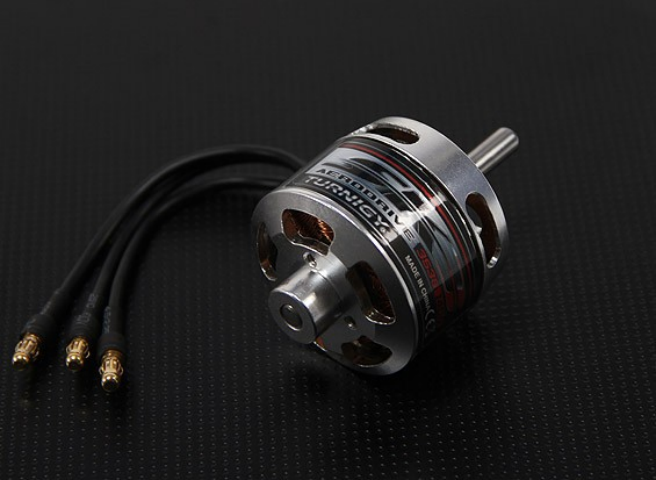
\includegraphics[width=0.45\textwidth]{figures/02_hardware/turnigy_motor.jpg}
		\caption{Turnigy Aereo Drive SK3 3536 1400 KV}
		\label{fig:turnigy_motor}
	\end{figure}
	
	%--------------------------------------------------------------
	\section{Turnigy Plush 40A. Electronic Speed Controller}
	Il \textbf{Turnigy Plush 40A} \cite{turnigy_plush} è un controllore elettronico di velocità per motori \textit{brushless BLDC}. Il suo compito è convertire la tensione continua di alimentazione nelle tre fasi necessarie al pilotaggio del motore. Il dispositivo è di tipo \textit{sensorless}: la posizione del rotore viene stimata indirettamente attraverso la forza controelettromotrice, senza impiegare sensori dedicati. Il comando di velocità viene invece ricevuto dal microcontrollore sotto forma di segnale PWM, sulla base del quale l'ESC genera la corretta sequenza di commutazione delle fasi. Nel \textit{Double Propeller Ducted Fan} sono impiegati due \textit{Turnigy Plush 40A}, uno per ciascun motore; il componente è riportato in Figura~\ref{fig:turnigy_plush}.
	
	\subsection{Turnigy Plush 40A. Caratteristiche fisiche}
	\begin{itemize}
		\item Corrente nominale: 40 [A].
		\item Corrente di picco: 55 [A].
		\item Presenza di un \textit{Battery Eliminator Circuit (BEC)}: 5 [V] a 3 [A].
		\item Celle di batteria necessarie per il corretto funzionamento del dispositivo: $[2 \div 6]$.
		\item Peso: 39 [g].
		\item Dimensioni in [mm]: $60\times 24\times 15$.
	\end{itemize}
	
	\begin{figure}[H]
		\centering
		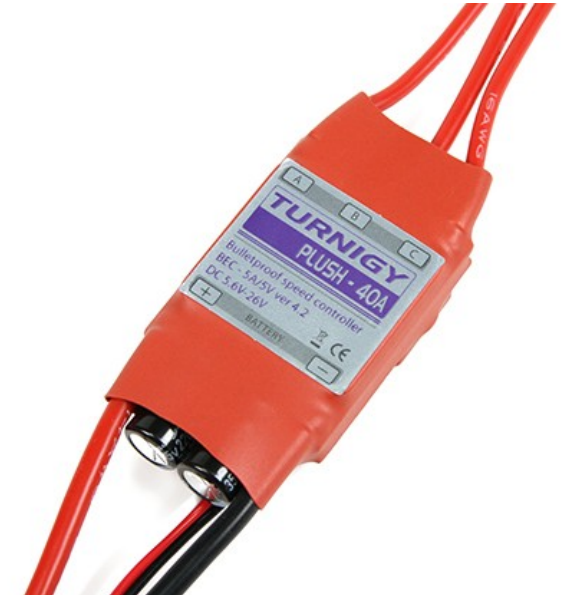
\includegraphics[width=0.45\textwidth]{figures/02_hardware/turnigy_plush_40a.jpg}
		\caption{Turnigy Plush 40A}
		\label{fig:turnigy_plush}
	\end{figure}
	
	\subsection{Turnigy Plush 40A. Risoluzione e controllo dei motori}
	L'ESC \textit{Turnigy Plush 40A} gestisce la potenza erogata ai motori mediante un segnale di controllo PWM (\textit{Pulse-Width Modulation}) operante a una frequenza di \textbf{50 [Hz]}. Prima di consentire l'azionamento dei rotori, il dispositivo impone l'esecuzione di una rigorosa procedura di sicurezza definita \textbf{armamento} (\textit{arming}), la quale viene innescata fornendo in ingresso un segnale PWM con un \textit{duty cycle} costantemente mantenuto al \textbf{5\%}.\\
	Lo stato operativo e l'esito della procedura di inizializzazione vengono comunicati all'operatore attraverso una diagnostica basata su specifici \textit{feedback} acustici emessi dall'ESC stesso:
	
	\paragraph{Attesa di un segnale di armamento valido}\mbox{}\\
	Un'emissione sonora ripetuta con una cadenza di due secondi segnala che l'ESC è correttamente alimentato dal lato di potenza, ma non rileva sul canale di controllo un segnale PWM idoneo a consentire l'armamento (ovvero il comando di "motore al minimo").
	
	\paragraph{Esito positivo dell'operazione di armamento}\mbox{}\\
	L'avvenuto sblocco di sicurezza e la conseguente operatività del sistema propulsivo sono confermati in modo inequivocabile da una sequenza composta da tre segnali acustici brevi, seguiti da una singola emissione prolungata.
	
	\paragraph{Esito negativo dell'operazione di armamento}\mbox{}\\
	Una rapida e ininterrotta sequenza di segnali sonori evidenzia una condizione di anomalia o un errore nella procedura di inizializzazione. Tale eventualità è tipicamente riconducibile al rilevamento di un valore iniziale del segnale PWM non conforme ai requisiti di sicurezza, oppure a un incremento troppo repentino del \textit{duty cycle} prima che il sistema si sia stabilizzato.\\
	
	Sulla base delle evidenze sperimentali raccolte durante le fasi preliminari di collaudo, è emersa l'opportunità di mantenere il segnale di armamento costante per un intervallo temporale compreso tra i \textbf{2} e i \textbf{6 [s]} prima di impartire effettivi comandi di trazione. Inoltre, la caratterizzazione pratica del sistema propulsivo ha permesso di definire che l'intervallo di lavoro utile dei motori, ai fini della generazione della spinta per il \textit{DPDF}, corrisponde a un \textit{duty cycle} strettamente circoscritto tra il \textbf{5\% e il 10\%}.
	
	%--------------------------------------------------------------
	\section{APC 9x4.5. Eliche}
	
	\subsection{Caratteristiche fisiche}
	\begin{itemize}
		\item Diametro: 9 [in], pari a 228.6 [mm].
		\item Passo: 4.5 [in], pari a 114.3 [mm].
		\item Peso: 17.9 [g].
		\item Materiale: Nylon rinforzato con fibra di vetro (\textit{Fiberglass-Reinforced Nylon, FRN}).
	\end{itemize}
	La geometria dell'elica impiegata è riportata in Figura~\ref{fig:apc_propeller}.
	
	\begin{figure}[H]
		\centering
		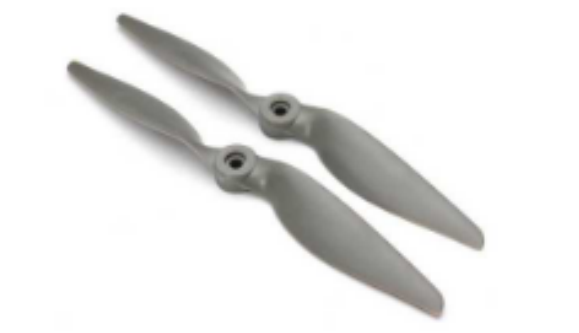
\includegraphics[width=0.45\textwidth]{figures/02_hardware/apc_9x45.jpg}
		\caption{Elica APC 9x4.5}
		\label{fig:apc_propeller}
	\end{figure}
	
	%--------------------------------------------------------------
	\section{Hitec HS-82MG Gear micro servo}
	Come discusso nella descrizione della struttura meccanica, il controllo dell'assetto in \textit{roll} e \textit{pitch} è affidato a due \textit{flap} montati nella parte inferiore del condotto. Tali superfici, investite dal getto prodotto dai motori controrotanti, generano l'azione aerodinamica correttiva necessaria a contrastare le rotazioni indesiderate del velivolo. Il movimento di ciascun \textit{flap} è affidato a un servomotore dedicato, in particolare nel progetto sono stati integrati due servomotori \textbf{Hitec HS-82MG} \cite{hitec_hs82mg}.
	
	\subsection{HS-82MG Hitec. Caratteristiche fisiche}
	\begin{itemize}
		\item Dimensioni: $29.8\times 12.0\times 29.6$ [mm].
		\item Peso: 19.0 [g].
	\end{itemize}
	Le dimensioni del servomotore sono riportate in Figura~\ref{fig:hs82mg_misure}.
	
	\begin{figure}[H]
		\centering
		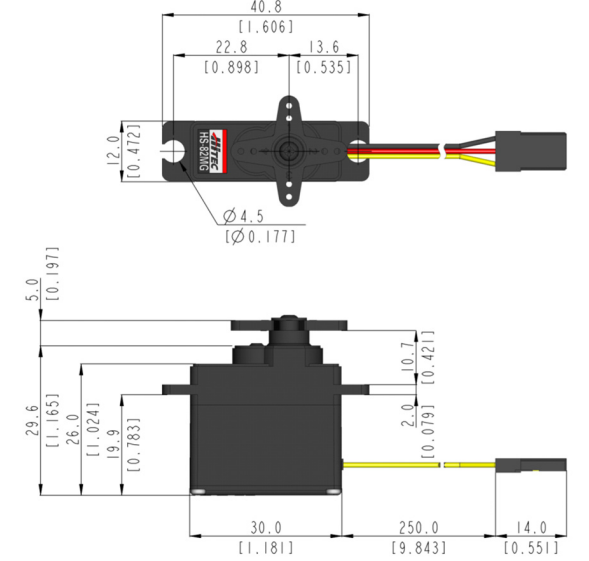
\includegraphics[width=0.5\textwidth]{figures/02_hardware/hs82mg_misure.png}
		\caption{HS-82MG Hitec. Misure}
		\label{fig:hs82mg_misure}
	\end{figure}
	
	\paragraph{Coppia di stasi (\textit{Holding torque})}\mbox{}\\
	Rappresenta il momento torcente massimo che il servomotore è in grado di esercitare per mantenere fissa la propria posizione angolare, contrastando in modo statico una sollecitazione meccanica esterna. Per il modello \textit{HS-82}, tale parametro si attesta a \textbf{2.2 [kg$\cdot$cm]} con un'alimentazione di \textbf{4.8 [V]}, incrementandosi fino a \textbf{2.7 [kg$\cdot$cm]} qualora la tensione di ingresso venga elevata a \textbf{6.0 [V]}.
	
	\paragraph{Coppia di stallo (\textit{Stall torque})}\mbox{}\\
	Definisce il momento torcente massimo teorico che l'attuatore è in grado di sviluppare in condizioni di velocità angolare nulla, ovvero quando il rotore è bloccato da un carico inamovibile. I valori nominali garantiti per questo dispositivo sono pari a \textbf{2.8 [kg$\cdot$cm]} a \textbf{4.8 [V]} e \textbf{3.4 [kg$\cdot$cm]} a \textbf{6.0 [V]}.
	
	\paragraph{Velocità angolare}\mbox{}\\
	Indica il tempo richiesto per compiere una determinata escursione angolare in assenza di carico meccanico. Alimentato a una tensione di \textbf{4.8 [V]}, il servomotore copre un angolo di 60\degree{} in \textbf{0.12 [s]}; elevando l'alimentazione a \textbf{6.0 [V]}, il tempo di rotazione si riduce a \textbf{0.10 [s]}. Esprimendo il dato in relazione a un singolo grado di variazione, si ottiene un tempo di azionamento pari a \textbf{0.0020 [s/\degree]} a \textbf{4.8 [V]} e \textbf{0.0017 [s/\degree]} a \textbf{6.0 [V]}.
	
	\paragraph{Corrente operativa}\mbox{}\\
	Rappresenta l'assorbimento medio di corrente del servomotore durante la sua normale movimentazione (misurato in assenza di carico applicato all'albero). In tali condizioni, durante un'escursione di 60\degree, si registra un assorbimento di \textbf{220 [mA]} operando a \textbf{4.8 [V]}, valore che sale a \textbf{280 [mA]} se il dispositivo è alimentato a \textbf{6.0 [V]}.
	
	\paragraph{Corrente di stallo}\mbox{}\\
	Costituisce l'assorbimento massimo di corrente che si verifica quando il motore è alimentato ma si trova in una condizione di blocco meccanico forzato. In questa situazione critica, la richiesta di corrente raggiunge i \textbf{1450 [mA]} con un'alimentazione a \textbf{4.8 [V]}, e si eleva fino a \textbf{1800 [mA]} a \textbf{6.0 [V]}.
	
	\paragraph{Corsa operativa}\mbox{}\\
	Fa riferimento all'escursione angolare totale che il servomotore è in grado di coprire in risposta a un segnale di comando PWM standard. Nel caso specifico del modello \textit{HS-82}, tale intervallo utile è pari a \textbf{120\degree}. Una rappresentazione visiva dell'attuatore è riportata in Figura~\ref{fig:hs82mg}.
	
	\begin{figure}[H]
		\centering
		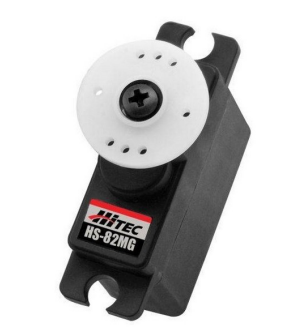
\includegraphics[width=0.4\textwidth]{figures/02_hardware/hs82mg.jpg}
		\caption{HS-82MG}
		\label{fig:hs82mg}
	\end{figure}
	
	\subsection{HS-82MG Hitec. Caratteristiche tecniche e controllo}
	
	\paragraph{Alimentazione}\mbox{}\\
	L'attuatore opera in un intervallo di tensione nominale compreso tra \textbf{4.8 e 6.0 [V]}. Sebbene l'impiego di tensioni prossime al limite superiore consenta un sensibile miglioramento delle prestazioni dinamiche del dispositivo, tale configurazione comporta un incremento della dissipazione termica per effetto Joule e un maggiore \textit{stress} a carico della circuiteria elettronica interna. Al fine di garantire un equilibrio ottimale tra reattività e affidabilità del sistema nel tempo, si è scelto di stabilizzare la tensione di alimentazione in ingresso al valore di \textbf{5 [V]}.
	
	\paragraph{Controllo}\mbox{}\\
	La regolazione della posizione angolare del rotore è affidata a un segnale di controllo di tipo PWM (\textit{Pulse-Width Modulation}). Per l'interfacciamento con il microcontrollore, è stata selezionata una frequenza di commutazione pari a \textbf{50 [Hz]}, con un'ampiezza di segnale di \textbf{3.3 [V]}.\\
	L'architettura di controllo è stata definita per soddisfare i seguenti requisiti operativi:
	\begin{itemize}
		\item \textbf{Configurazione neutra}: per ottenere il posizionamento dei \textit{flap} in configurazione iniziale (perfettamente perpendicolari al piano del suolo), è necessario fornire un impulso di attivazione con durata pari a \textbf{1.5 [ms]}, corrispondente a un \textit{duty cycle} del \textbf{7.5\%}.
		\item \textbf{Rotazione oraria}: l'escursione angolare in senso orario viene comandata modulando la durata dell'impulso nell'intervallo compreso tra \textbf{1.5} e \textbf{2.1 [ms]}.
		\item \textbf{Rotazione antioraria}: specularmente, il movimento in senso antiorario si ottiene operando nell'intervallo di temporizzazione tra \textbf{0.9} e \textbf{1.5 [ms]}.
	\end{itemize}
	La disposizione dei terminali di collegamento del servomotore e la relativa piedinatura sono illustrate in Figura~\ref{fig:hs82mg_terminali}.
	
	\begin{figure}[H]
		\centering
		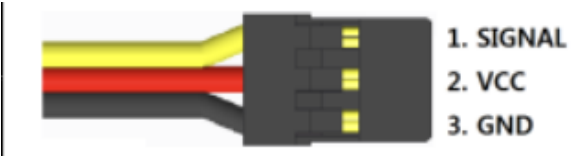
\includegraphics[width=0.5\textwidth]{figures/02_hardware/hs82mg_terminali.png}
		\caption{HS-82MG Hitec. Disposizione dei terminali}
		\label{fig:hs82mg_terminali}
	\end{figure}
	
	%--------------------------------------------------------------
	\section{BNO055 Bosch Sensortec. Unità di misura inerziale e magnetometro}
	Per garantire un accurato controllo dell'assetto del \textit{DPDF}, risulta indispensabile conoscere in tempo reale l'esatto orientamento del sistema rispetto a una terna di riferimento spaziale fissa. Si rende pertanto necessario l'impiego di un dispositivo in grado di rilevare ed elaborare tale informazione cinematica. Il \textbf{BNO055}, prodotto da \textit{Bosch Sensortec}, è un sensore di orientamento assoluto a 9 assi che, grazie alla sua elevata accuratezza e al notevole livello di integrazione, rappresenta la soluzione hardware ideale per questo scopo.\\
	Il dispositivo si configura come un \textit{System in Package (SiP)} il quale, come documentato nel \textit{datasheet} ufficiale \cite{bno055_ds}, integra al proprio interno: un accelerometro triassiale a 14 bit, un giroscopio triassiale a 16 bit, un sensore geomagnetico triassiale e un microcontrollore a 32 bit basato su architettura \textit{Arm Cortex-M0+}. Il compito primario di tale microcontrollore è l'esecuzione \textit{on-board} di un avanzato algoritmo proprietario di \textit{sensor fusion}.\\
	Questo algoritmo elabora e combina in tempo reale i dati grezzi provenienti dall'accelerometro, dal giroscopio e dal magnetometro, filtrando i disturbi e fornendo direttamente in uscita misure di assetto stabili e precise. Tali dati possono essere estratti sotto forma di quaternioni oppure come angoli di Eulero (rollio, beccheggio e imbardata, ovvero \textit{roll, pitch} e \textit{yaw}), unitamente ai vettori di accelerazione lineare e gravitazionale.\\
	Nel contesto del presente progetto, il chip \textit{BNO055} è stato adottato nella sua versione preassemblata su un'apposita scheda di \textit{breakout}, soluzione che ne semplifica notevolmente l'interfacciamento e il cablaggio elettrico. Per maggiore completezza descrittiva, nei paragrafi successivi verranno riportate le caratteristiche dimensionali e di peso riferite sia al singolo chip sia all'intero modulo di \textit{breakout}.
	
	\subsection{BNO055 Bosch Sensortec. Caratteristiche fisiche}
	\begin{itemize}
		\item Dimensioni del modulo: $20\times 24\times 2$ mm.
		\item Dimensioni del chip: $3.8\times 5.2\times 1.1$ mm.
		\item Massa del modulo: 3 g.
		\item Massa del chip: $\approx 150$ mg.
	\end{itemize}
	
	\subsection{BNO055 Bosch Sensortec. Infrastruttura di alimentazione, comunicazione ed integrazione del sensore}
	
	\paragraph{Alimentazione}\mbox{}\\
	Il chip \textit{BNO055} dispone di due pin di alimentazione distinti, denominati \textbf{VDD} e \textbf{VDDIO}, dedicati rispettivamente all'alimentazione della circuiteria interna del sensore e delle interfacce logiche digitali. I relativi intervalli di tensione operativa sono compresi tra \textbf{2.4 e 3.6 [V]} per il terminale \textit{VDD}, e tra \textbf{1.7 e 3.6 [V]} per il terminale \textit{VDDIO}. Tuttavia, impiegando il dispositivo preassemblato su scheda di \textit{breakout}, tali ingressi vengono gestiti e unificati internamente dalla circuiteria della scheda stessa. Di conseguenza, l'alimentazione all'intero modulo viene fornita attraverso un unico terminale di ingresso, denominato \textbf{VIN}, che accetta tensioni comprese nell'intervallo $2.4 \div 3.6$ [V]. Tra i diversi profili di gestione energetica previsti dal costruttore, per lo sviluppo del progetto si è optato per la configurazione in \textbf{\textit{Normal mode}}, al fine di garantire la piena e continua operatività del sensore.
	
	\paragraph{Protocollo di comunicazione}\mbox{}\\
	Per quanto concerne l'interfacciamento con il microcontrollore \textit{host}, il \textit{BNO055} supporta nativamente i protocolli di comunicazione seriale $I^{2}C$ e \textit{UART}. Per le specifiche esigenze architetturali del \textit{DPDF}, l'acquisizione della telemetria inerziale è stata implementata avvalendosi esclusivamente del bus di comunicazione $I^{2}C$. Il sensore è compatibile sia con la trasmissione in \textit{Standard Mode}, operante a una frequenza di clock di \textbf{100 [kHz]}, sia in \textit{Fast Mode}, raggiungendo velocità fino a \textbf{400 [kHz]}. Sia il sensore integrato sia la relativa \textit{breakout board} espongono i terminali standard \textbf{SDA} (\textit{Serial Data}) e \textbf{SCL} (\textit{Serial Clock}) necessari per instaurare la comunicazione digitale. La mappatura completa dei pin (\textit{pinout}) del modulo utilizzato è richiamata in Figura~\ref{fig:bno055_breakout}.
	
	\begin{figure}[H]
		\centering
		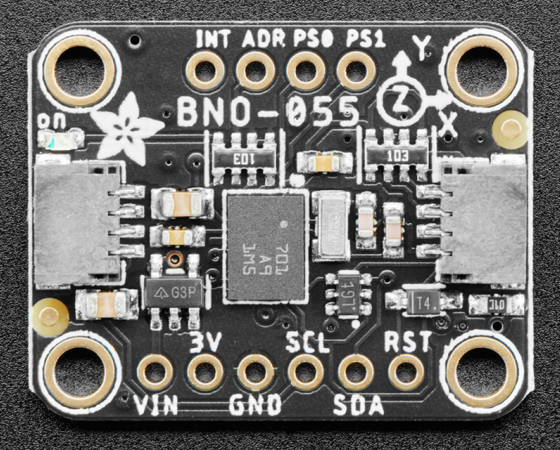
\includegraphics[width=0.45\textwidth]{figures/02_hardware/bno055_breakout.jpg}
		\caption{BNO055 Bosch Sensortec. Configurazione dei pin e breakout board}
		\label{fig:bno055_breakout}
	\end{figure}
	
	\subsection{BNO055 Bosch Sensortec. Sensori inerziali e sensor fusion}
	Il \textit{BNO055} integra al proprio interno un accelerometro, un giroscopio e un magnetometro in un singolo dispositivo, combinandone le misurazioni attraverso un algoritmo proprietario di \textit{sensor fusion}. Nello specifico, l'accelerometro è un sensore \textbf{MEMS} capacitivo dedicato alla misurazione dell'accelerazione lineare lungo i tre assi; il giroscopio è un sensore MEMS a struttura vibrante preposto al rilevamento della velocità angolare; infine, il magnetometro rileva il campo magnetico terrestre, fornendo un riferimento assoluto per l'orientamento spaziale. L'architettura di sistema del sensore è schematizzata in Figura~\ref{fig:bno055_arch}.
	
	\paragraph{Accelerometro}\mbox{}\\
	Il modulo accelerometrico presenta una risoluzione di \textbf{14 bit} e supporta fondoscale di misura selezionabili tra $\pm 2$ [g], $\pm 4$ [g], $\pm 8$ [g] e $\pm 16$ [g]. Ai fini del progetto, il sensore è stato configurato con un intervallo operativo di \textbf{$\pm 4$ [g]} e una banda passante di \textbf{62.5 [Hz]}.
	
	\paragraph{Giroscopio}\mbox{}\\
	Il giroscopio integrato vanta una risoluzione di \textbf{16 bit} e mette a disposizione intervalli di misura compresi tra $\pm 125$ [\degree/s] e $\pm 2000$ [\degree/s]. Abilitando l'algoritmo di \textit{sensor fusion}, il dispositivo adotta automaticamente il fondoscala massimo di \textbf{$\pm 2000$ [\degree/s]}, operando con una banda passante di \textbf{32 [Hz]}.
	
	\paragraph{Magnetometro}\mbox{}\\
	Il magnetometro è in grado di rilevare intensità di campo magnetico fino a $\pm 1300$ [$\mu$T] lungo gli assi X e Y, e fino a $\pm 2500$ [$\mu$T] lungo l'asse Z. La risoluzione della misura è pari a \textbf{13 bit} per gli assi planari (X, Y) e a \textbf{15 bit} per l'asse verticale (Z). Quando l'algoritmo di \textit{sensor fusion} è attivo, la banda passante operativa del magnetometro è impostata a \textbf{10 [Hz]}.
	
	\paragraph{Sensor fusion}\mbox{}\\
	Presi singolarmente, i tre trasduttori inerziali presentano limiti fisici intrinseci e complementari: il giroscopio è soggetto a deriva temporale (\textit{drift}), l'accelerometro risente fortemente delle accelerazioni lineari non gravitazionali (come vibrazioni e transitori del telaio) e il magnetometro è altamente sensibile alle perturbazioni elettromagnetiche ambientali. La logica di \textit{sensor fusion} sfrutta congiuntamente i dati grezzi provenienti dai tre componenti per elaborare una stima dell'orientamento nettamente più stabile, robusta e affidabile.\\
	Come riportato nella documentazione tecnica del \textit{BNO055}, tale elaborazione matematica si fonda sull'implementazione di un \textbf{Filtro di Kalman Esteso (EKF)}. Nel presente lavoro, questa modalità è stata mantenuta costantemente attiva; nello specifico, l'architettura di controllo sviluppata sfrutta direttamente le stime degli angoli di rollio, beccheggio e imbardata (\textit{roll, pitch} e \textit{yaw}) calcolate \textit{on-board} dal sensore, mentre non si è reso necessario l'impiego diretto delle ulteriori grandezze cinematiche disponibili. A seguire, è riportata una rappresentazione schematica del \textit{System in Package BNO055} sviluppato da \textit{Bosch Sensortec}.
	
	\begin{figure}[H]
		\centering
		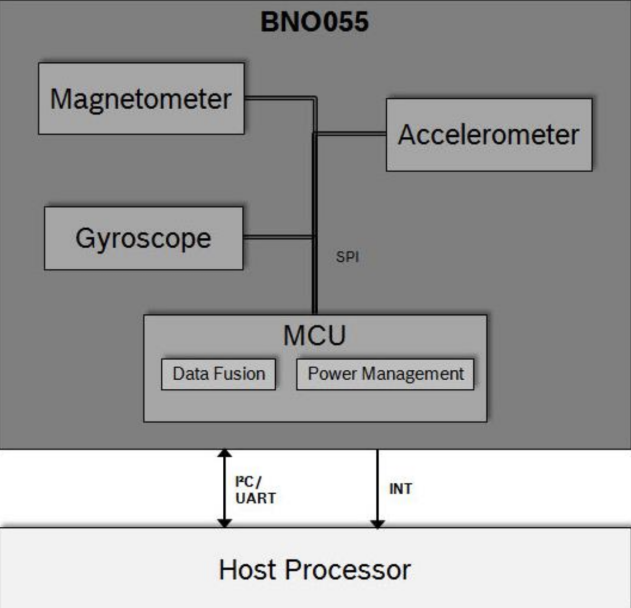
\includegraphics[width=0.6\textwidth]{figures/02_hardware/bno055_architettura.png}
		\caption{BNO055 Bosch Sensortec. Architettura di sistema}
		\label{fig:bno055_arch}
	\end{figure}
	
	\subsection{BNO055 Bosch Sensortec. Modalità operative}
	
	\paragraph{Modalità operative con Sensor Fusion (\textit{Fusion Modes})}\mbox{}\\
	Quando il dispositivo viene configurato in una delle modalità operative provviste di \textit{sensor fusion}, l'algoritmo interno esegue automaticamente, in \textit{background}, la calibrazione continua dei trasduttori. Le modalità disponibili sono le seguenti:
	\begin{itemize}
		\item \textbf{IMU}: stima l'orientamento spaziale combinando esclusivamente i dati dell'accelerometro e del giroscopio. Grazie alla sua elevata reattività, questa modalità risulta particolarmente indicata per applicazioni altamente dinamiche.
		\item \textbf{M4G (\textit{Magnetometer for Gyroscope})}: presenta un comportamento analogo alla modalità IMU, ma impiega il magnetometro in sostituzione del giroscopio per correggere la stima dell'orientamento, vincolandola al campo magnetico terrestre.
		\item \textbf{COMPASS}: il dispositivo opera come una bussola elettronica a stato solido, fornendo una stima dell'orientamento sul piano orizzontale riferita al Nord magnetico.
		\item \textbf{NDOF (\textit{Nine Degrees of Freedom})}: sfrutta congiuntamente i dati provenienti da tutti e tre i sensori (accelerometro, giroscopio e magnetometro) per restituire la stima dell'orientamento assoluto più accurata e completa possibile.
	\end{itemize}
	
	\paragraph{Modalità operative senza Sensor Fusion (\textit{Non-Fusion Modes})}\mbox{}\\
	Le modalità operative prive di fusione sensoriale consentono all'utente di acquisire direttamente i dati grezzi (\textit{raw data}) misurati dai singoli trasduttori o da specifiche combinazioni di essi, aggirando del tutto l'algoritmo di elaborazione interna.\\
	Nello specifico, il dispositivo può essere configurato per abilitare esclusivamente l'accelerometro (\textbf{ACCONLY}), il magnetometro (\textbf{MAGONLY}) o il giroscopio (\textbf{GYROONLY}), oppure per attivare specifiche coppie di sensori (\textbf{ACCMAG, ACCGYRO, MAGGYRO}). Infine, la modalità \textbf{AMG} abilita simultaneamente tutti e tre i trasduttori, demandando tuttavia l'onere computazionale dell'eventuale fusione dei dati al microcontrollore \textit{host} esterno.\\
	Ai fini dello sviluppo del presente progetto, tali configurazioni a dati grezzi non sono state impiegate. La scelta progettuale è infatti ricaduta in modo esclusivo sulla modalità di fusione \textbf{NDOF}, ritenuta la soluzione più idonea ed efficiente per demandare al sensore il calcolo dell'assetto e ottenere direttamente una stima stabile e affidabile dell'orientamento del drone.
	
	%--------------------------------------------------------------
	\section{VL53L1X ST. Sensore Time-of-Flight per la misurazione a lunga distanza}
	Al fine di controllare correttamente il \textit{DPDF}, è necessario stimare la distanza dal suolo durante il volo. Per questo scopo è stato adottato il \textbf{VL53L1X} di \textit{STMicroelectronics} \cite{vl53l1x_ds}. Nel progetto non è stato utilizzato il sensore in forma nativa, ma il modulo \textit{IRIS11A0J9776} prodotto da \textit{Pololu}, scelto per semplificare l'integrazione elettronica grazie alla relativa \textit{breakout board}.
	
	\subsection{Il principio di misura di un sensore Time-of-Flight (ToF)}
	La misura \textit{Time-of-Flight} si basa sul tempo impiegato da un impulso luminoso per compiere un tragitto di andata e ritorno tra il sensore e l'oggetto da rilevare. Nel caso del \textit{VL53L1X}, l'emissione avviene tramite un laser \textbf{VCSEL}, mentre la radiazione riflessa viene raccolta da un rilevatore sensibile, tipicamente uno \textbf{SPAD array}. Una volta noto il tempo di volo $\Delta t$, la distanza si ricava da:
	\begin{equation}
		d = \frac{c \cdot \Delta t}{2}
		\label{eq:tof}
	\end{equation}
	dove $d$ è la distanza dall'oggetto e $c$ è la velocità della luce. Il fattore 2 tiene conto del percorso di andata e ritorno del segnale. Nel caso in esame, il \textit{VL53L1X} utilizza la tecnologia \textbf{dToF (\textit{Direct Time-of-Flight})}, adatta a misure di distanza accurate e robuste per il controllo di quota del sistema.
	
	\subsection{VL53L1X STMicroelectronics. Caratteristiche fisiche}
	A seguire, un breve elenco delle principali caratteristiche fisiche:
	\begin{itemize}
		\item Dimensioni del chip: $4.90\times 1.25\times 1.56$ [mm].
		\item Dimensioni del modulo: $17.50\times 12\times 2.56$ [mm].
		\item Massa del chip: 30 [mg].
		\item Massa del modulo: 0.5 [g] (senza i \textit{pin header}).
	\end{itemize}
	
	\subsection{VL53L1X STMicroelectronics. Caratteristiche tecniche}
	
	\paragraph{Alimentazione}\mbox{}\\
	Il \textit{VL53L1X} presenta un unico ingresso di alimentazione, indicato come \textbf{VDD}, con intervallo operativo $[2.6 \div 3.5]$ [V].
	
	\paragraph{Protocollo di comunicazione}\mbox{}\\
	Il sensore comunica esclusivamente tramite protocollo $I^{2}C$ e supporta la \textit{Fast Mode} a \textbf{400 [kHz]}. I terminali messi a disposizione per la comunicazione sono \textbf{SDA} e \textbf{SCL}.
	
	\paragraph{XSHUT e GPIO 1 (Interrupt)}\mbox{}\\
	Il \textit{VL53L1X} dispone dell'ingresso \textbf{XSHUT}, usato per spegnimento, riavvio o reset hardware del dispositivo, e dell'uscita \textbf{GPIO1}, utilizzata come linea di \textit{interrupt} per segnalare eventi al microcontrollore. Nel progetto, \textbf{XSHUT} è stato impiegato per il reset forzato del sensore, mentre \textbf{GPIO1} è stato usato per notificare la disponibilità di una nuova misura, semplificando la gestione firmware e la temporizzazione. La configurazione dei pin del modulo e lo schema a blocchi del sensore sono riportati in Figura~\ref{fig:vl53l1x_pinout}.\\
	Il dettaglio dell'emettitore ottico del sensore è mostrato in Figura~\ref{fig:vl53l1x_emettitore}.
	
	\begin{figure}[H]
		\centering
		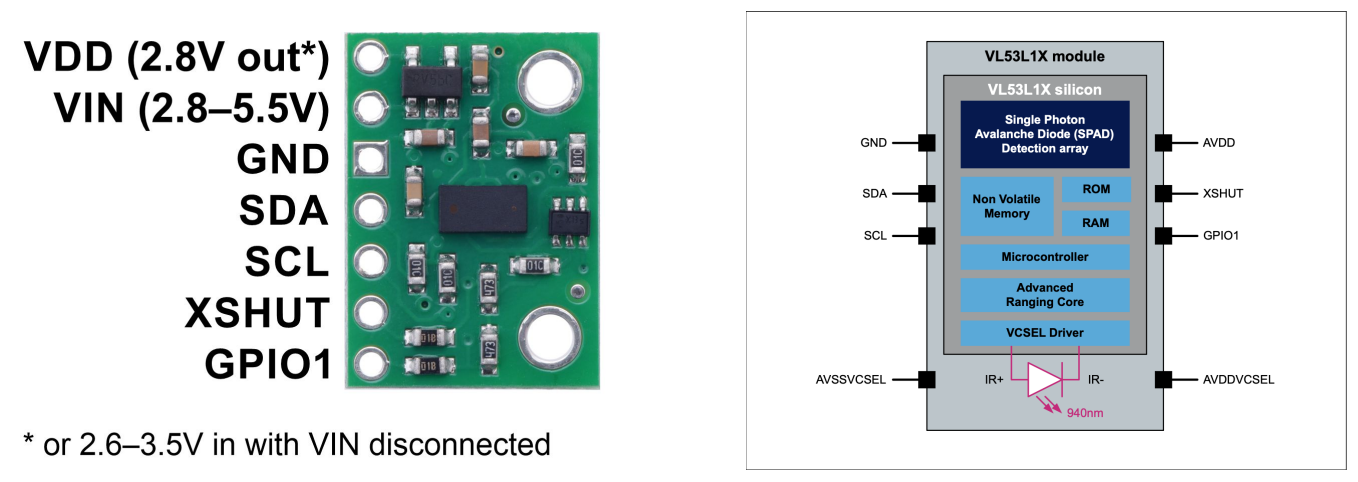
\includegraphics[width=0.95\textwidth]{figures/02_hardware/vl53l1x_pinout.png}
		\caption{Pin Configuration (sinistra) e System Block Diagram (destra) del VL53L1X}
		\label{fig:vl53l1x_pinout}
	\end{figure}
	
	\begin{figure}[H]
		\centering
		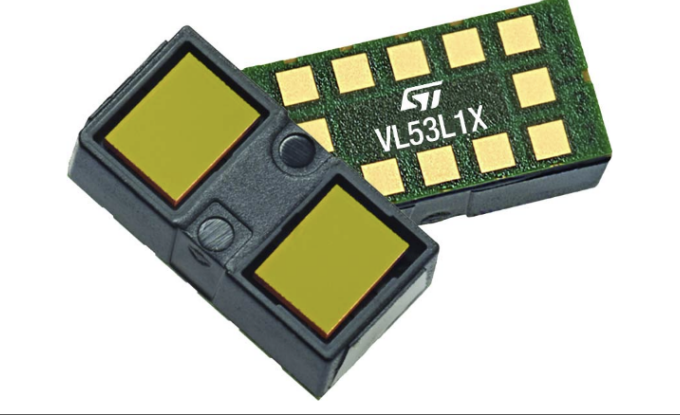
\includegraphics[width=0.45\textwidth]{figures/02_hardware/vl53l1x_emettitore.jpg}
		\caption{VL53L1X, dettaglio sull'emettitore}
		\label{fig:vl53l1x_emettitore}
	\end{figure}
	
	\paragraph{Field of View e Region of Interest}\mbox{}\\
	Il \textit{Field of View} rappresenta l'angolo massimo entro il quale il dispositivo è in grado di rilevare un oggetto; per il sensore in esame, il \textbf{FoV} è pari a circa \textbf{27\degree}. Il \textit{VL53L1X} mette inoltre a disposizione la funzione \textbf{Region of Interest (R.O.I.)}, che consente di restringere il \textit{Field of View} effettivamente utilizzato durante la misura, risultando utile soprattutto nel caso di oggetti di piccole dimensioni. Nel presente progetto, tuttavia, il sensore è impiegato per la misura dell'altitudine del \textit{DPDF}; di conseguenza, la funzione R.O.I. non è stata utilizzata e il FoV è stato lasciato al valore nominale, come illustrato in Figura~\ref{fig:vl53l1x_fov}.
	
	\begin{figure}[H]
		\centering
		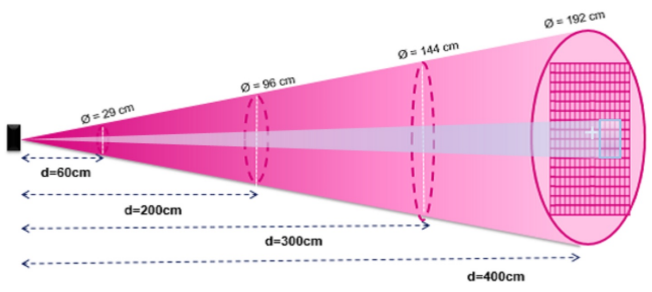
\includegraphics[width=0.7\textwidth]{figures/02_hardware/vl53l1x_fov.png}
		\caption{Field of View del VL53L1X}
		\label{fig:vl53l1x_fov}
	\end{figure}
	
	\paragraph{Prestazioni di misura, Timing Budget e modalità operative di misura}\mbox{}\\
	Il \textit{VL53L1X} offre buone prestazioni di misura in termini di accuratezza e rapidità. Il dispositivo è in grado di misurare distanze fino a \textbf{4 [m]}, con frequenze che possono arrivare fino a \textbf{50 [Hz]}. Per adattarsi a scenari applicativi differenti, il sensore consente di selezionare la modalità di misura più adatta, bilanciando portata, robustezza e velocità di acquisizione. A seguire, una tabella riassuntiva delle modalità di misura offerte dal dispositivo, riportata in Tabella~\ref{tab:vl53l1x_modalita}:
	
	\begin{table}[H]
		\centering
		\begin{tabular}{l c c}
			\toprule
			\textbf{Modalità} & \textbf{\makecell{Range max in condizioni \\ di scarsa luce (approssimato)}} & \textbf{\makecell{Range max con \\ luce ambientale}} \\
			\midrule
			Short  & 136 [cm] & 135 [cm] \\
			Medium & 290 [cm] & 76 [cm]  \\
			Long   & 360 [cm] & 73 [cm]  \\
			\bottomrule
		\end{tabular}
		\caption{VL53L1X -- Modalità di misura}
		\label{tab:vl53l1x_modalita}
	\end{table}
	
	La modalità \textit{Short ranging} è progettata per acquisizioni ravvicinate, garantendo letture stabili e robuste anche in ambienti caratterizzati da forte luminosità. Al contrario, la modalità \textit{Long ranging} privilegia la massima portata spaziale, accettando tuttavia misurazioni intrinsecamente più sensibili al rumore ottico. Tra queste due opzioni estreme si colloca la configurazione \textit{Medium ranging}, che offre un compromesso bilanciato tra distanza operativa e robustezza del dato.\\
	Per soddisfare gli specifici requisiti del \textit{DPDF}, la scelta progettuale è ricaduta sulla modalità \textbf{Short ranging}, che è stata mantenuta come unica configurazione operativa per l'intera durata dello sviluppo e dei test.\\
	Al fine di gestire in modo ottimale il compromesso intrinseco tra velocità di campionamento e precisione della misura, si è fatto ricorso al parametro di \textbf{Timing Budget} del sensore. Con tale termine si definisce il tempo complessivo allocato al dispositivo per l'esecuzione di una singola misurazione di distanza. Questa grandezza è espressa in [ms] e può essere configurata su valori compresi nell'intervallo $20 \div 1000$ [ms]. All'aumentare del \textit{Timing Budget} corrisponde fisiologicamente una riduzione della frequenza di acquisizione; tuttavia, un tempo di integrazione ottica più lungo garantisce un netto miglioramento in termini di accuratezza e stabilità della lettura.\\
	La documentazione tecnica ufficiale suggerisce che un \textit{Timing Budget} pari a \textbf{33 [ms]} rappresenti un eccellente compromesso tra reattività dinamica e affidabilità del dato; pertanto, la configurazione del firmware è stata impostata su tale valore. A supporto di questa scelta costruttiva, in Figura~\ref{fig:vl53l1x_prestazioni} è riportato un grafico estratto direttamente dallo \textit{User Manual} del \textit{VL53L1X}, il quale illustra le prestazioni e l'andamento della misurazione a fronte di diversi valori del \textit{Timing Budget} adottato.
	
	\begin{figure}[H]
		\centering
		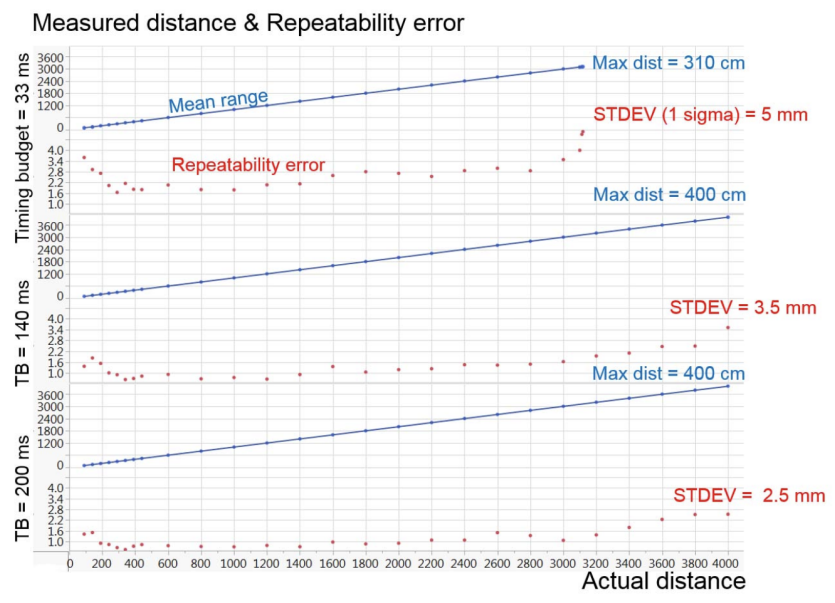
\includegraphics[width=0.75\textwidth]{figures/02_hardware/vl53l1x_prestazioni.png}
		\caption{VL53L1X, prestazioni di misura}
		\label{fig:vl53l1x_prestazioni}
	\end{figure}
	
	%--------------------------------------------------------------
	\section{Schema dei collegamenti}
	Lo schema elettrico complessivo del sistema è riportato in Figura~\ref{fig:schema_collegamenti}.
	
	\begin{figure}[H]
		\centering
		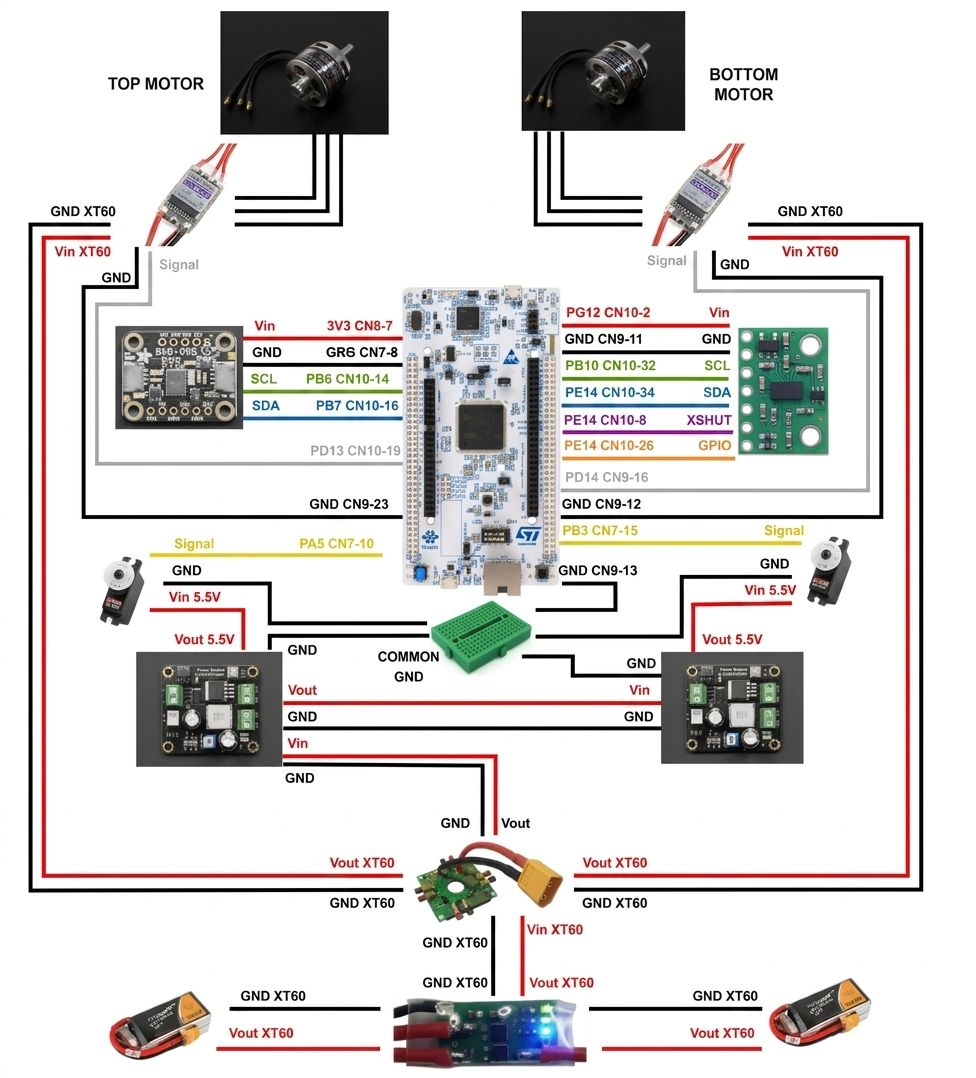
\includegraphics[width=0.95\textwidth]{figures/02_hardware/schema_collegamenti.png}
		\caption{Schema dei collegamenti}
		\label{fig:schema_collegamenti}
	\end{figure}
	
	\subsection{Tabelle dei collegamenti}
	Di seguito vengono dettagliati i collegamenti elettrici intercorrenti tra i principali componenti hardware del sistema e la scheda di controllo centrale. Le tabelle presentate in questa sezione sono state richiamate puntualmente nel testo per agevolare la consultazione e garantire la replicabilità dell'architettura hardware.
	
	\paragraph{Collegamenti tra NUCLEO-H745ZI-Q e sensore VL53L1X}\mbox{}\\
	Il sensore di distanza \textit{VL53L1X} (STMicroelectronics) è stato interfacciato direttamente alla scheda \textit{NUCLEO-H745ZI-Q}. Il dettaglio delle connessioni pin-to-pin è riportato nella Tabella~\ref{tab:coll_vl53l1x}.
	
	\begin{table}[H]
		\centering
		\begin{tabular}{l l}
			\toprule
			\textbf{VL53L1X} & \textbf{NUCLEO-H745ZI-Q} \\
			\midrule
			Vin & PG12, CN10-2 \\
			GND & GND, CN10-5 \\
			SCL & SCL I2C2: PB10, CN10-32 \\
			SDA & SDA I2C2: PB11, CN10-34 \\
			XSHUT & PE14, CN10-8 \\
			GPIO & CN10-26 \\
			\bottomrule
		\end{tabular}
		\caption{Collegamenti NUCLEO-H745ZI-Q e VL53L1X}
		\label{tab:coll_vl53l1x}
	\end{table}
	
	\paragraph{Collegamenti tra NUCLEO-H745ZI-Q e sensore BNO055}\mbox{}\\
	Analogamente, anche l'unità inerziale \textit{BNO055} (Bosch Sensortec) è stata collegata in modo diretto alla piattaforma di controllo. Lo schema di cablaggio adottato è sintetizzato nella Tabella~\ref{tab:coll_bno055}.
	
	\begin{table}[H]
		\centering
		\begin{tabular}{l l}
			\toprule
			\textbf{BNO055} & \textbf{NUCLEO-H745ZI-Q} \\
			\midrule
			Vin & 3.3V, CN8-7 \\
			GND & GND, CN8-11 \\
			SCL & SCL I2C1: PB6, CN10-14 \\
			SDA & SDA I2C1: PB7, CN10-16 \\
			\bottomrule
		\end{tabular}
		\caption{Collegamenti NUCLEO-H745ZI-Q e BNO055}
		\label{tab:coll_bno055}
	\end{table}
	
	\paragraph{Collegamenti tra convertitori (DFRobot), servomotori e NUCLEO-H745ZI-Q}\mbox{}\\
	Al fine di garantire il corretto azionamento del comparto servomotori, risulta essenziale stabilire un riferimento di massa comune. Per tale ragione, è stata impiegata una \textit{breadboard} esterna funzionante da nodo di distribuzione per la massa (GND) proveniente dalla \textit{NUCLEO-H745ZI-Q} (pin CN7-8). L'alimentazione di potenza dei servomotori è stata invece prelevata direttamente dai terminali di uscita dei convertitori di tensione collegati in serie. Le configurazioni di cablaggio per il servo deputato al controllo del rollio (\textit{roll}) e per quello del beccheggio (\textit{pitch}) sono riportate rispettivamente in Tabella~\ref{tab:coll_roll_servo} e Tabella~\ref{tab:coll_pitch_servo}.
	
	\begin{table}[H]
		\centering
		\begin{tabular}{l l l l}
			\toprule
			\textbf{DF-Robot (Roll)} & \textbf{Roll-servo} & \textbf{Massa Comune} & \textbf{NUCLEO-H745ZI-Q} \\
			\midrule
			Vout-3   & Vin (5.5V) & -    & - \\
			Vout-GND & GND        & C.GND & GND, CN7-8 \\
			-        & Signal     & -    & TIM2-CH1: PA5, CN7-10 \\
			\bottomrule
		\end{tabular}
		\caption{Collegamenti NUCLEO-H745ZI-Q e Roll-servo}
		\label{tab:coll_roll_servo}
	\end{table}
	
	\begin{table}[H]
		\centering
		\begin{tabular}{l l l l}
			\toprule
			\textbf{DF-Robot (Pitch)} & \textbf{Pitch-servo} & \textbf{Massa Comune} & \textbf{NUCLEO-H745ZI-Q} \\
			\midrule
			Vout-3   & Vin (5.5V) & -    & - \\
			Vout-GND & GND        & C.GND & GND, CN7-8 \\
			-        & Signal     & -    & TIM2-CH2: PB3, CN7-15 \\
			\bottomrule
		\end{tabular}
		\caption{Collegamenti NUCLEO-H745ZI-Q e Pitch-servo}
		\label{tab:coll_pitch_servo}
	\end{table}
	
	\paragraph{Collegamenti tra Power Distribution Module, ESC e NUCLEO-H745ZI-Q}\mbox{}\\
	Per quanto concerne il comparto propulsivo, gli ESC ricevono l'alimentazione dal \textit{Power Distribution Module}, il quale è a sua volta interfacciato al comparto batterie (PSM) e ai motori tramite connettori trifase dedicati. Anche in questo caso è tassativo che il terminale di massa degli ESC sia equipotenziale rispetto alla massa della \textit{NUCLEO-H745ZI-Q}, mentre il terminale del segnale logico deve essere connesso al rispettivo pin PWM della scheda. I cablaggi afferenti all'ESC del motore superiore (\textit{Top-motor}) e a quello inferiore (\textit{Bottom-motor}) sono illustrati nelle Tabelle~\ref{tab:coll_top_esc} e~\ref{tab:coll_bottom_esc}.
	
	\begin{table}[H]
		\centering
		\begin{tabular}{l l l}
			\toprule
			\textbf{Power Distribution Module} & \textbf{Top-motor-ESC} & \textbf{NUCLEO-H745ZI-Q} \\
			\midrule
			Vout XT-60 & Vin XT-60 & - \\
			GND XT-60  & GND XT-60 & - \\
			-          & Signal    & TIM4-CH2: PD13, CN10-19 \\
			-          & GND       & GND \\
			\bottomrule
		\end{tabular}
		\caption{Collegamenti NUCLEO-H745ZI-Q e Top-motor-ESC}
		\label{tab:coll_top_esc}
	\end{table}
	
	\begin{table}[H]
		\centering
		\begin{tabular}{l l l}
			\toprule
			\textbf{Power Distribution Module} & \textbf{Bottom-motor-ESC} & \textbf{NUCLEO-H745ZI-Q} \\
			\midrule
			Vout XT-60 & Vin XT-60 & - \\
			GND XT-60  & GND XT-60 & - \\
			-          & Signal    & TIM4-CH3: PD14, CN9-16 \\
			-          & GND       & GND \\
			\bottomrule
		\end{tabular}
		\caption{Collegamenti NUCLEO-H745ZI-Q e Bottom-motor-ESC}
		\label{tab:coll_bottom_esc}
	\end{table}
	
	\textit{Nota}: il dispositivo che riceve il segnale PWM deve condividere lo stesso riferimento di massa del dispositivo che genera tale segnale.

    %%%%%%%%%%%%%%%%%%%%%%%%%%%%%%%%%%%%%%%%%%%%%%%%%%%%%%%%%%%%%%%%%%%%
	%                         CAPITOLO 3 - FIRMWARE
	%%%%%%%%%%%%%%%%%%%%%%%%%%%%%%%%%%%%%%%%%%%%%%%%%%%%%%%%%%%%%%%%%%%%
	\chapter{Firmware}
	\label{ch:firmware}
	
	Il presente capitolo illustra l'architettura software sviluppata per la gestione e il controllo del \textit{Double Propeller Ducted-Fan (DPDF)}. Il firmware è stato concepito non come un sistema di controllo a sé stante, ma come componente di una pipeline più ampia che comprende l'acquisizione strutturata dei dati, l'identificazione del modello dinamico in ambiente MATLAB e la successiva validazione dei regolatori sul prototipo fisico. Per questa ragione, il microcontrollore non si limita a calcolare l'azione di controllo: deve allo stesso tempo trasmettere al PC ospite un flusso di telemetria stabile, ricevere comandi in tempo reale e garantire la sicurezza del sistema in ogni fase operativa.\\
	Per soddisfare questi requisiti, il firmware è stato strutturato secondo un'architettura modulare ed \textit{event-driven} che garantisce tre proprietà fondamentali:
	\begin{enumerate}
		\item un \textbf{campionamento deterministico} delle grandezze di stato (angoli di Eulero forniti dalla IMU \textit{BNO-055} e quota fornita dal ToF \textit{VL53L1X}), con jitter di fase contenuto;
		\item un \textbf{sistema di telemetria ad alta frequenza}, capace di trasmettere a 50 [Hz] su porta seriale a 230\,400 [baud] lo stato completo del sistema --- inclusi angoli, quota, comandi PWM applicati agli attuatori, contatori di errore UART e \textit{flag} di stato;
		\item un'\textbf{infrastruttura di controllo flessibile}, predisposta per ricevere dall'esterno sia i comandi di prova durante la fase di identificazione, sia i guadagni dei PID derivati dalla simulazione per la successiva validazione sperimentale.
	\end{enumerate}
	Nelle sezioni che seguono vengono descritte, in ordine, l'architettura software complessiva, la gestione del microcontrollore \textit{dual-core}, l'organizzazione modulare del codice, la configurazione delle periferiche, la gestione dei sensori, i diagrammi di flusso del sistema, l'architettura di controllo a quattro PID e il protocollo di comunicazione seriale con MATLAB.
	
	%--------------------------------------------------------------
	\section{Architettura software \textit{event-driven}}
	\label{sec:architettura_software}
	
	L'infrastruttura firmware sviluppata per il \textit{DPDF} si fonda su un'architettura \textit{event-driven}, ovvero guidata dagli eventi temporali e hardware. A differenza dei paradigmi puramente sequenziali, basati sul \textit{polling} continuo dei sensori, l'architettura adottata fa sì che l'unità di calcolo intervenga esclusivamente quando si verifica un evento rilevante: la disponibilità di una nuova misura dal sensore di quota, la scadenza del timer che governa il ciclo di assetto, oppure l'arrivo di un comando dalla porta seriale.\\
	Per garantire questa reattività, le \textit{Interrupt Service Routine (ISR)} associate a \textit{timer} e periferiche sono state mantenute estremamente leggere. Il loro unico compito è quello di alzare una \textit{flag} logica di attivazione (ad esempio \texttt{flag\_int\_servo\_control = true}), senza eseguire calcoli o accessi a periferiche che potrebbero protrarne la durata. L'elaborazione vera e propria --- acquisizione dati via $I^{2}C$, filtraggio, calcolo dei PID e aggiornamento dei registri PWM --- viene invece eseguita nel ciclo principale \texttt{while(1)}, che monitora costantemente lo stato delle \textit{flag} ed esegue i blocchi computazionali pesanti solo quando il rispettivo sottosistema lo richiede.\\
	Questa separazione tra \textit{eventi} (gestiti in ISR) ed \textit{elaborazione} (gestita nel \textit{main loop}) presenta tre vantaggi concreti per il presente progetto. In primo luogo, riduce la latenza di risposta agli eventi più critici, perché le ISR completano in pochi microsecondi e lasciano il core libero. In secondo luogo, evita situazioni di \textit{race condition} sui dati condivisi, perché l'elaborazione avviene sempre nel contesto sequenziale del \textit{main loop}. Infine, rende il sistema più facilmente verificabile: ogni evento corrisponde a una \textit{flag}, ogni \textit{flag} a un blocco di codice ben identificabile, e l'ordine di esecuzione è esplicito.
	
	%--------------------------------------------------------------
	\section{Gestione del microcontrollore \textit{dual-core}}
	\label{sec:dual_core}
	
	Il microcontrollore \textit{STM32H745ZI-TQ6}, descritto nel Capitolo~\ref{ch:hardware}, è caratterizzato da un'architettura \textit{dual-core} che integra un processore \textit{Arm Cortex-M7} e un coprocessore \textit{Arm Cortex-M4}. Sebbene l'intera logica di controllo sia eseguita dal \textit{Cortex-M4}, anche il \textit{Cortex-M7} riveste un ruolo essenziale nella fase di avvio del sistema.\\
	Per ragioni architetturali interne al microcontrollore, la configurazione del clock e l'inizializzazione della \textit{Power Domain} principale sono di esclusiva competenza del \textit{Cortex-M7}, in quanto core primario. Il \textit{Cortex-M4} resta dunque in attesa, in modalità a basso consumo (\textit{Wait For Event, WFE}), fino a quando il \textit{Cortex-M7} non gli segnala il completamento di tale configurazione tramite un \textit{Hardware Semaphore (HSEM)}. Solo dopo aver ricevuto questo segnale, il \textit{Cortex-M4} esce dallo stato di attesa e procede con l'inizializzazione delle proprie periferiche e con l'avvio del \textit{main loop} di controllo.\\
	Una conseguenza pratica di questa architettura, di particolare rilevanza in fase di sviluppo, riguarda la procedura di \textit{flashing} del firmware. Il binario destinato al \textit{Cortex-M7} deve essere caricato \textit{prima} di quello destinato al \textit{Cortex-M4}: in caso contrario, il \textit{Cortex-M4} rimane indefinitamente bloccato in attesa del segnale \textit{HSEM} che non verrà mai generato, e il sistema risulta apparentemente non operativo. L'ambiente di sviluppo \textit{STM32CubeIDE} consente di gestire entrambi i target all'interno dello stesso progetto, garantendo la corretta sequenza di programmazione.
	
	%--------------------------------------------------------------
	\section{Organizzazione modulare del codice}
	\label{sec:organizzazione_codice}
	
	Per favorire la leggibilità, la manutenibilità e la verificabilità del firmware, il codice sorgente è stato organizzato in moduli funzionalmente coesi. Ogni modulo è composto da un \textit{header file} (\texttt{.h}), che dichiara l'interfaccia pubblica del modulo, e da un \textit{source file} (\texttt{.c}), che ne contiene l'implementazione. Le configurazioni di basso livello generate da \textit{STM32CubeMX} sono state mantenute separate dai moduli applicativi, in modo da non appesantire il file \texttt{main.c} con dettagli implementativi delle periferiche.\\
	I principali moduli applicativi sviluppati sono i seguenti:
	\begin{itemize}
		\item \textbf{\texttt{main.c}} --- contiene la sequenza di inizializzazione del sistema, il \textit{safe startup}, il \textit{main loop} basato sulle \textit{flag} di evento e la chiamata coordinata agli altri moduli.
		\item \textbf{\texttt{config.h} e \texttt{config.c}} --- raccolgono in un unico punto i parametri numerici che descrivono il comportamento ammissibile del sistema: limiti PWM per motori e servomotori, posizione neutra dei servo, fattori di conversione angolo--PWM, parametri di sicurezza, riferimenti e guadagni dei quattro PID. Centralizzare queste costanti rende esplicito il confine tra legge di controllo e limiti imposti dall'hardware reale, ed evita la dispersione di valori magici nel codice.
		\item \textbf{\texttt{pwm.c}} --- incapsula la gestione dei segnali PWM destinati a motori (\texttt{TIM4-CH2}, \texttt{TIM4-CH3}) e servomotori (\texttt{TIM2-CH1}, \texttt{TIM2-CH2}). Espone funzioni di alto livello per impostare un comando in unità fisiche (angolo flap, valore CCR motore), che internamente effettuano la saturazione hardware e l'aggiornamento dei \textit{Capture-Compare Register} del rispettivo \textit{timer}.
		\item \textbf{\texttt{pid.c}} --- implementa un'unica classe di regolatore PID a tempo discreto, di cui sono istanziate quattro versioni indipendenti --- per quota, \textit{roll}, \textit{pitch} e \textit{yaw} --- ciascuna con i propri guadagni e il proprio stato interno (termine integrale accumulato, errore precedente, derivata filtrata).
		\item \textbf{\texttt{imu.c}} --- costituisce un livello di astrazione sopra il \textit{driver} ufficiale Bosch del sensore \textit{BNO-055}. Si occupa dell'inizializzazione, dell'impostazione della modalità operativa, della lettura periodica degli angoli di Eulero e della loro conversione in centesimi di grado per la trasmissione via UART.
		\item \textbf{\texttt{altimetro.h}} --- definisce le costanti fisiche e i parametri di filtraggio impiegati nell'elaborazione della misura di quota fornita dal \textit{VL53L1X}, inclusi i parametri della compensazione geometrica rispetto all'inclinazione del velivolo.
		\item \textbf{\texttt{cmd\_parser.c} e \texttt{cmd\_parser.h}} --- implementano la macchina a stati che riceve, valida ed esegue i comandi inviati dal PC sulla porta seriale, gestendo sia i comandi periodici di attuazione (\texttt{CMD,top,bottom,roll,pitch}) sia i comandi di stato (\texttt{MOTOR\_ON}, \texttt{MOTOR\_OFF}, \texttt{KILL}).
	\end{itemize}
	
	Questa suddivisione consente, in fase di sviluppo, di intervenire su un modulo alla volta riducendo il rischio di introdurre regressioni in funzionalità già validate. Le modifiche al firmware sono state pertanto effettuate come modifiche puntuali e mirate, conservando per quanto possibile la struttura e le interfacce esistenti.
	
	%--------------------------------------------------------------
	\section{Configurazione delle periferiche}
	\label{sec:periferiche}
	
	La configurazione hardware del \textit{Cortex-M4} è stata generata tramite \textit{STM32CubeMX} a partire dal file di progetto \texttt{.ioc}, ed è stata mantenuta coerente con i collegamenti pin-to-pin descritti nel Capitolo~\ref{ch:hardware}. Si descrivono di seguito le periferiche principali impiegate dal firmware.
	
	\subsection{Timer}
	I quattro \textit{timer} impiegati svolgono ruoli funzionalmente distinti:
	\begin{itemize}
		\item \textbf{TIM2}: configurato in modalità \textit{PWM Generation}, genera sui canali CH1 e CH2 i segnali di controllo dei servomotori di \textit{roll} e \textit{pitch}. Frequenza di funzionamento pari a \textbf{50 [Hz]}, coerente con le specifiche dei servo \textit{HS-82MG}.
		\item \textbf{TIM4}: anch'esso in modalità \textit{PWM Generation}, genera sui canali CH2 e CH3 i segnali destinati agli ESC \textit{Turnigy Plush 40A} che pilotano i due motori \textit{brushless}. Frequenza di 50 [Hz] richiesta dagli ESC stessi.
		\item \textbf{TIM6}: impiegato per la sequenza temporizzata di \textit{safe startup} (descritta nella Sezione~\ref{sec:safe_startup}) e per il pilotaggio diagnostico dei LED integrati sulla scheda.
		\item \textbf{TIM7}: utilizzato come \textit{timebase} per la generazione periodica dell'\textit{interrupt} che innesca l'aggiornamento del ramo di controllo IMU--servomotori. La sua scadenza alza la \textit{flag} \texttt{flag\_int\_servo\_control}, che il \textit{main loop} intercetta per eseguire la lettura del BNO-055, il calcolo dei PID di assetto e l'aggiornamento del PWM dei servo.
	\end{itemize}
	I valori di \textit{Prescaler} e \textit{Auto-Reload Register (ARR)} di ciascun \textit{timer} sono stati calcolati a partire dalla frequenza di clock del bus APB1 (configurata a 75 [MHz]) secondo la relazione standard:
	\begin{equation}
		f_{PWM} = \frac{f_{clk}}{(\textit{Prescaler}+1) \cdot (\textit{ARR}+1)}
		\label{eq:freq_pwm}
	\end{equation}
	
	\subsection{Periferiche di comunicazione}
	Il firmware utilizza due canali distinti per la comunicazione:
	\begin{itemize}
		\item \textbf{USART3}: configurata in modalità \textit{full-duplex} asincrona a \textbf{230\,400 [baud]} con \textbf{8 bit di dato, 1 bit di stop, nessuna parità}. Questo canale costituisce il collegamento bidirezionale con il PC ospite: in trasmissione veicola la telemetria a 50 [Hz], in ricezione raccoglie i comandi inviati da MATLAB. La scelta di un \textit{baud rate} elevato è motivata dalla necessità di non saturare il canale alla frequenza di telemetria adottata, considerando che ogni pacchetto è composto da una stringa CSV di lunghezza variabile.
		\item \textbf{$I^{2}C1$ e $I^{2}C2$}: configurati in \textit{Fast Mode} a \textbf{400 [kHz]}, dedicati rispettivamente alla comunicazione con il sensore \textit{BNO-055} e con il sensore \textit{VL53L1X}. L'impiego di due bus distinti, anziché di un unico bus condiviso, evita conflitti di indirizzo e permette di gestire i due sensori in modo completamente indipendente.
	\end{itemize}
	La gestione degli \textit{interrupt} associati a queste periferiche è affidata al \textit{Nested Vectored Interrupt Controller (NVIC)}, configurato con livelli di priorità coerenti con la criticità temporale di ciascuna sorgente di evento.
	
	%--------------------------------------------------------------
	\section{Gestione dei sensori}
	\label{sec:gestione_sensori}
	
	\subsection{VL53L1X --- Acquisizione di quota}
	L'acquisizione della quota avviene tramite il sensore \textit{Time-of-Flight VL53L1X}, descritto nel Capitolo~\ref{ch:hardware}. Il firmware utilizza il \textit{driver} ufficiale fornito da \textit{STMicroelectronics}, integrato attraverso un sottile livello di adattamento alle funzioni HAL.\\
	La sequenza di inizializzazione del sensore prevede: il rilascio del segnale \texttt{XSHUT}, il caricamento del firmware interno tramite \texttt{VL53L1\_WaitDeviceBooted()}, l'inizializzazione tramite \texttt{VL53L1\_DataInit()}, l'impostazione della modalità \textit{Short ranging} e del \textit{Timing Budget} a \textbf{33 [ms]}, e infine l'avvio della misura continua tramite \texttt{VL53L1\_StartMeasurement()}.\\
	Per non bloccare il microcontrollore durante il tempo di integrazione ottica, l'acquisizione segue un approccio basato sulla disponibilità del dato. Ad ogni iterazione del ramo motori, il firmware interroga il sensore tramite \texttt{VL53L1\_GetMeasurementDataReady()}: se un nuovo dato è disponibile, la misura viene letta con \texttt{VL53L1\_GetRangingMeasurementData()} e l'\textit{interrupt} interno del sensore viene azzerato con \texttt{VL53L1\_ClearInterruptAndStartMeasurement()}, predisponendo il sensore per la lettura successiva. Se invece il dato non è ancora disponibile, il firmware prosegue senza bloccarsi, lasciando al sensore il tempo di completare l'integrazione.\\
	La misura grezza così ottenuta viene successivamente compensata rispetto all'inclinazione istantanea del velivolo, in modo da fornire al regolatore di quota una stima coerente con la variabile fisica realmente controllata --- la coordinata verticale --- piuttosto che con la distanza grezza misurata dal sensore lungo il proprio asse.
	
	\subsection{BNO-055 --- Acquisizione dell'assetto}
	Il \textit{BNO-055} è responsabile del monitoraggio dell'assetto tridimensionale del velivolo. Il firmware utilizza il \textit{driver} platform-agnostic fornito da \textit{Bosch Sensortec}, adattato al contesto HAL per le funzioni di comunicazione $I^{2}C$, di temporizzazione e di gestione del \textit{reset}.\\
	La sequenza di inizializzazione del sensore comprende: la verifica dell'identità del dispositivo tramite la lettura del registro \texttt{CHIP\_ID}, l'impostazione delle unità di misura (gradi per gli angoli, $m/s^{2}$ per le accelerazioni), e l'impostazione della modalità operativa. Come anticipato nel Capitolo~\ref{ch:hardware}, è stata scelta la modalità di \textit{fusion} \textbf{NDOF}, in cui l'algoritmo proprietario del sensore combina i dati provenienti da accelerometro, giroscopio e magnetometro per restituire una stima stabile e robusta dell'orientamento assoluto.\\
	Subito dopo l'inizializzazione, e prima dell'avvio del ciclo di controllo, il firmware acquisisce un campione di \textit{posa iniziale} tramite la funzione \texttt{DPDF\_BNO055\_firmware\_read\_init()}, che memorizza gli angoli di Eulero correnti come riferimento. Tutte le letture successive vengono espresse come scostamento rispetto a questa posa iniziale: in questo modo i PID di assetto lavorano su angoli \textit{relativi} alla configurazione di equilibrio meccanico in cui il drone si trova all'accensione, evitando la dipendenza dall'orientamento magnetico assoluto e semplificando il confronto con la simulazione.\\
	Le letture periodiche degli angoli avvengono nel ramo IMU--servo a 100 [Hz], frequenza coerente con la massima banda passante del \textit{sensor fusion} interno al BNO-055 in modalità NDOF. I valori vengono mantenuti internamente in centesimi di grado, formato che consente di trasmettere informazione angolare con precisione di $0.01\degree$ utilizzando soli interi a 16 bit nella stringa di telemetria.
	
	%--------------------------------------------------------------
	\section{Diagrammi di flusso}
	\label{sec:diagrammi_flusso}
	
	Per illustrare in modo sintetico la logica decisionale e le dipendenze temporali dei diversi \textit{task} del firmware, vengono di seguito presentati tre diagrammi di flusso: due dedicati alla gestione dei singoli sensori, e uno che sintetizza l'esecuzione complessiva del firmware.
	
	\subsection{Diagramma di flusso del VL53L1X}
	Il diagramma di Figura~\ref{fig:flow_vl53l1x} riassume la sequenza di inizializzazione e di acquisizione del sensore di quota. Il flusso si conclude con l'attivazione della modalità di misura continua, dopodiché il \textit{main loop} interroga periodicamente la disponibilità del dato senza bloccarsi.
	
	\begin{figure}[H]
		\centering
		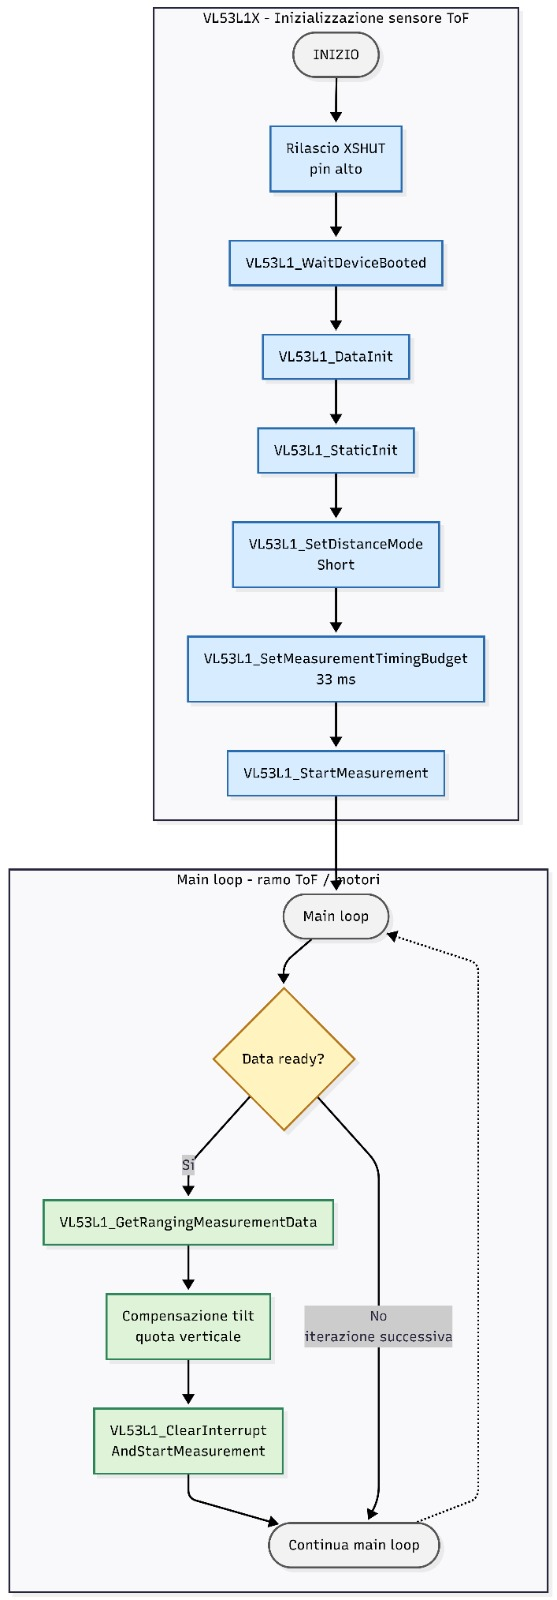
\includegraphics[width=0.4\textwidth]{figures/03_firmware/flow_vl53l1x.png}
		\caption{Diagramma di flusso del sensore VL53L1X}
		\label{fig:flow_vl53l1x}
	\end{figure}
	
	\subsection{Diagramma di flusso del BNO-055}
	Il diagramma di Figura~\ref{fig:flow_bno055} illustra la sequenza di astrazione dell'API Bosch. Particolarmente rilevante è il blocco dedicato all'acquisizione della posa iniziale (\texttt{DPDF\_BNO055\_firmware\_read\_init}), che fissa il sistema di riferimento angolare rispetto al quale tutte le misure successive saranno espresse.
	
	\begin{figure}[H]
		\centering
		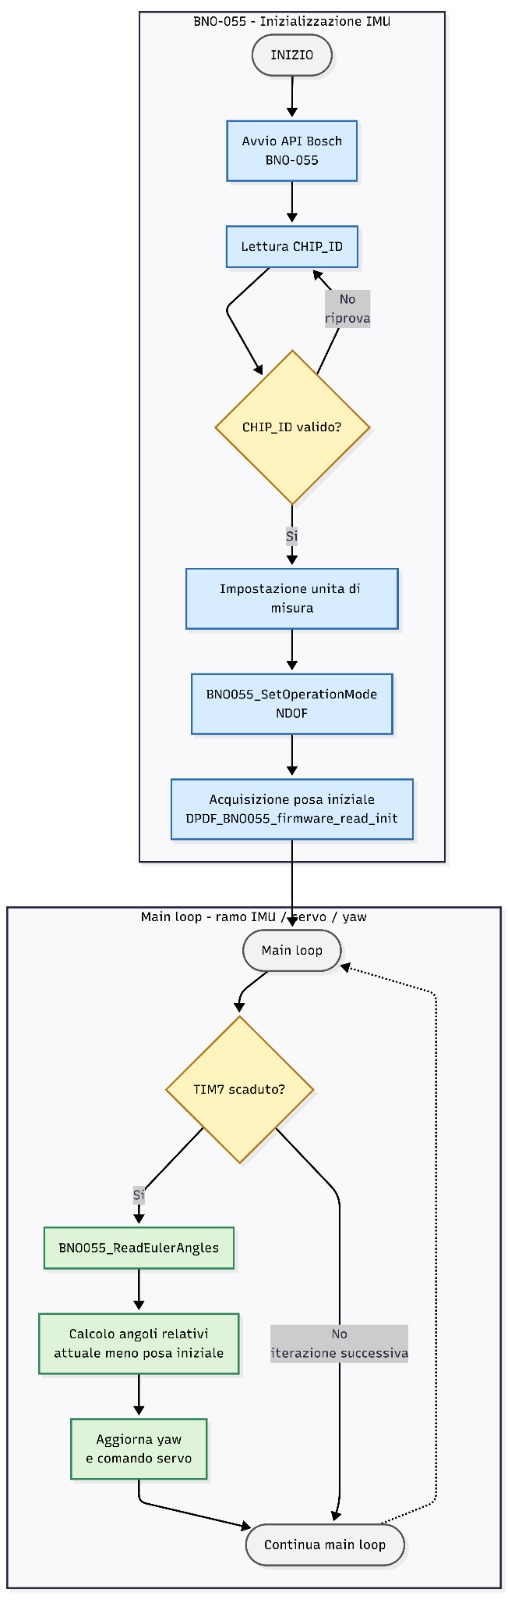
\includegraphics[width=0.35\textwidth]{figures/03_firmware/flow_bno055.png}
		\caption{Diagramma di flusso del sensore BNO-055}
		\label{fig:flow_bno055}
	\end{figure}
	
	\subsection{Diagramma di flusso del firmware complessivo}
	
	\begin{figure}[H]
		\centering
		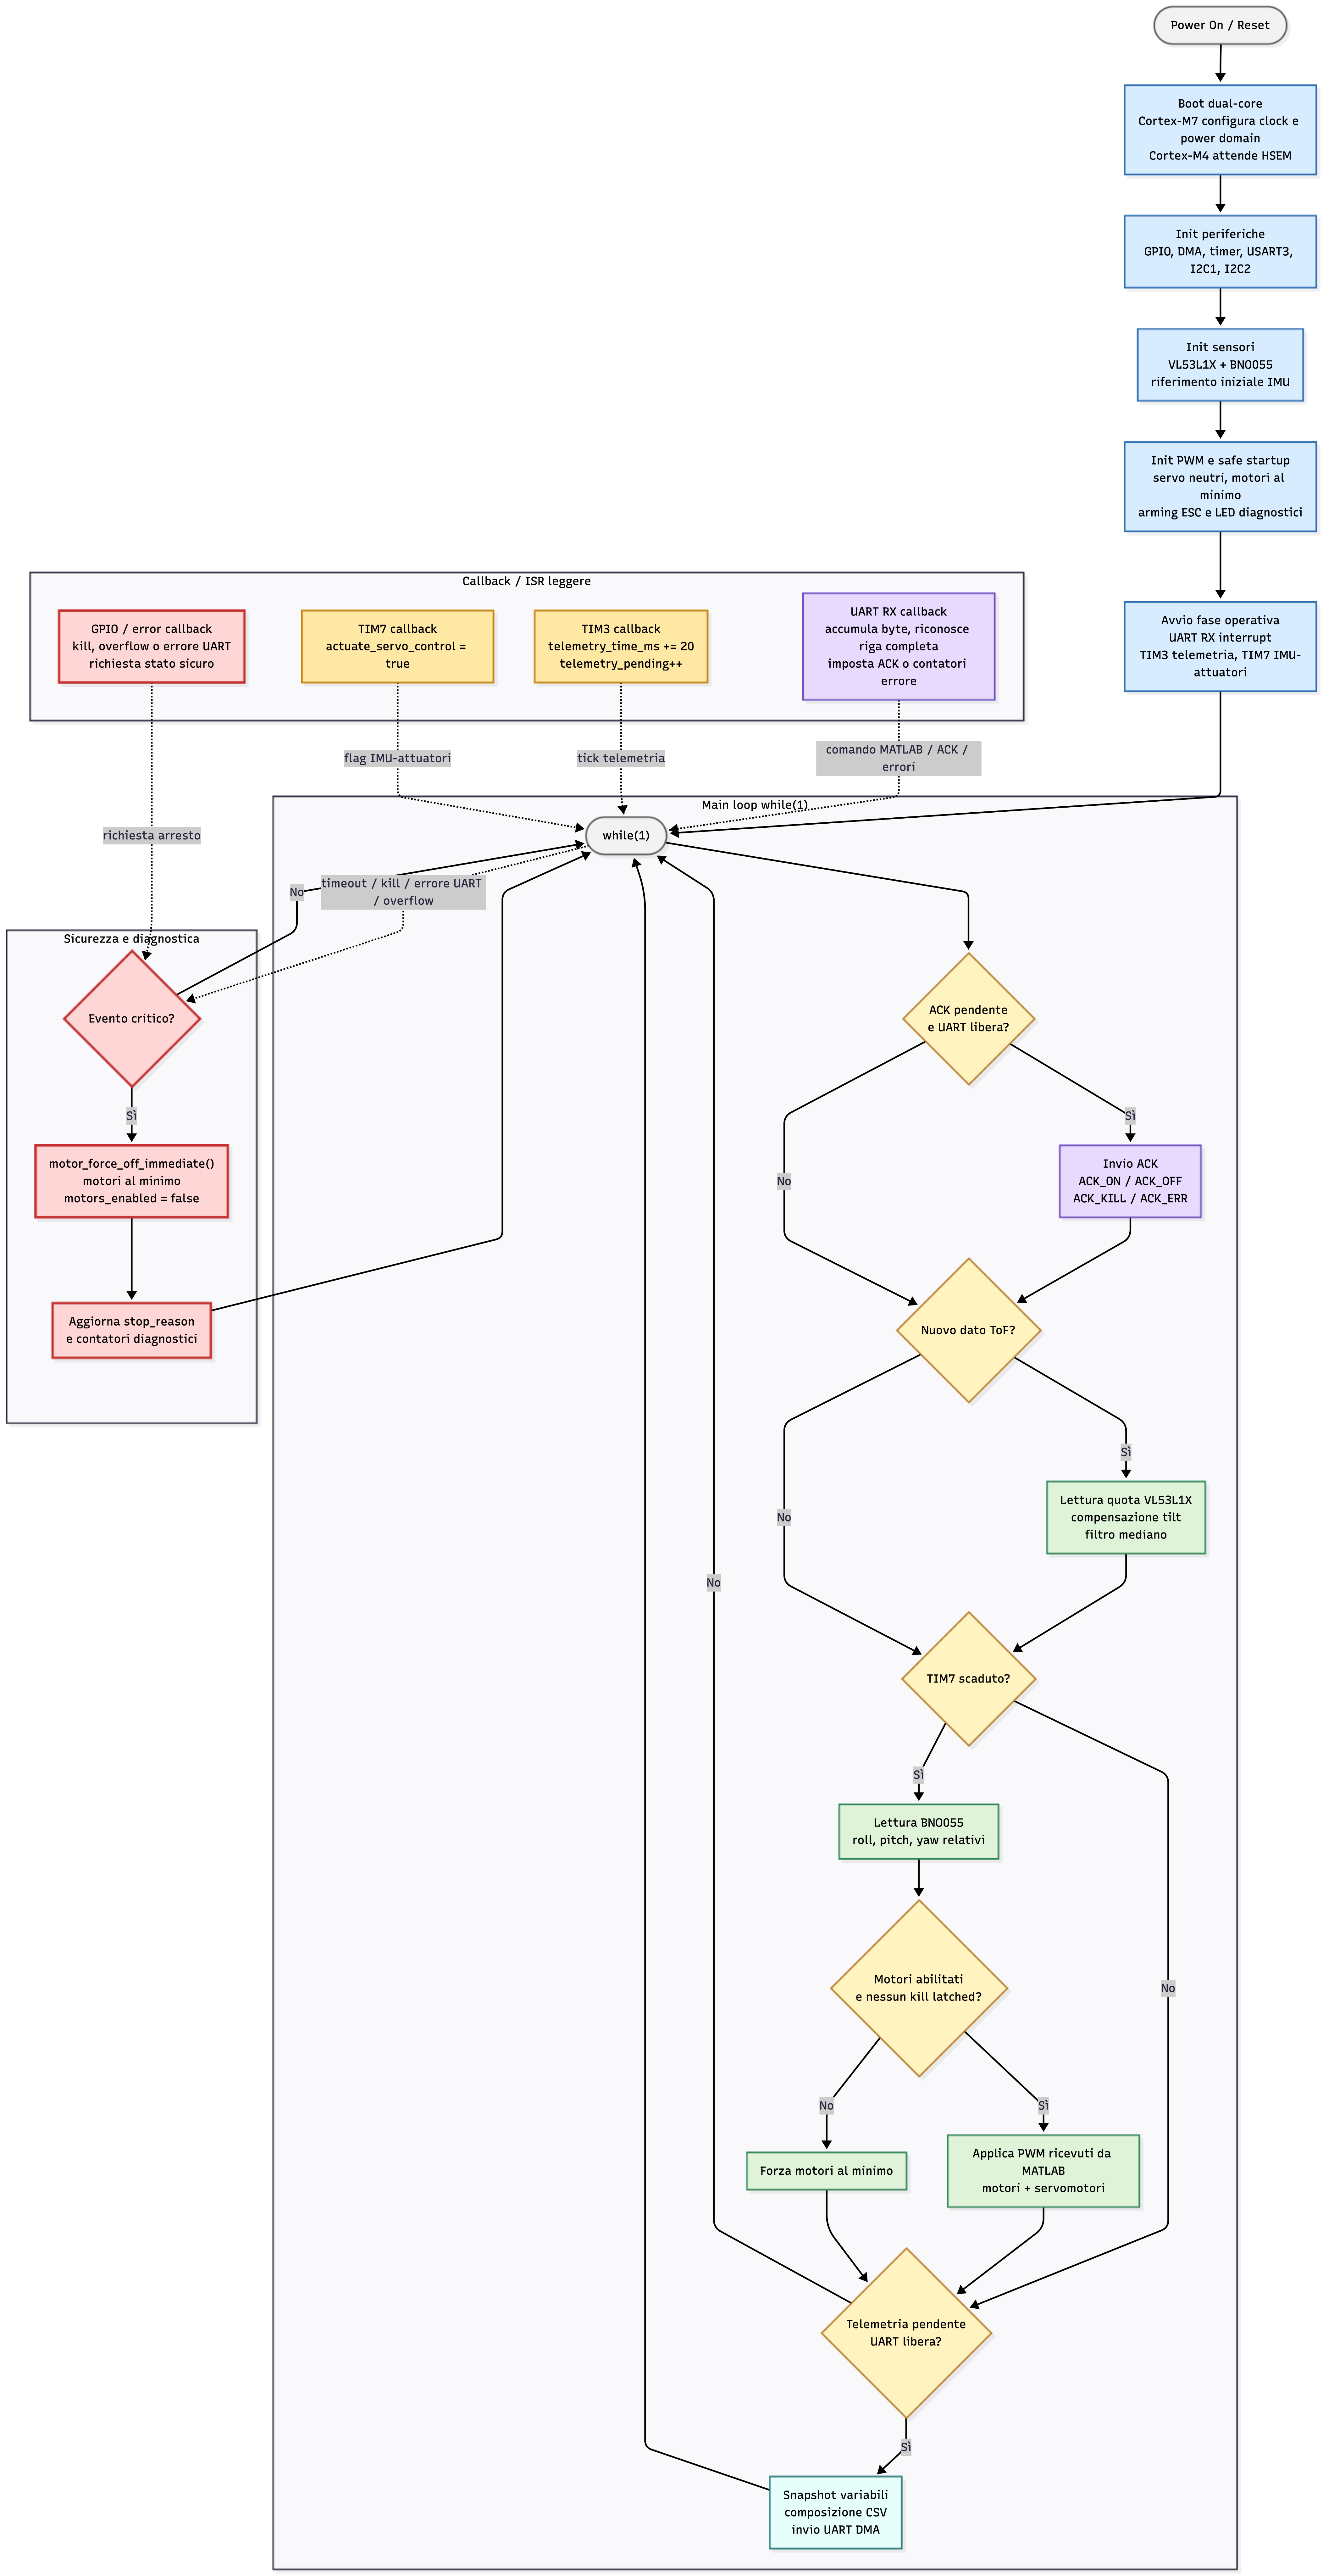
\includegraphics[width=0.75\textwidth] {figures/03_firmware/flow_complessivo.png}
		\caption{Diagramma di flusso complessivo del firmware}
		\label{fig:flow_complessivo}
	\end{figure}
	
		Il diagramma di Figura~\ref{fig:flow_complessivo} sintetizza la cooperazione tra i moduli software. Il flusso si articola in due macro-fasi:
	\begin{enumerate}
		\item \textbf{Inizializzazione e \textit{safe startup}}: il sistema attende un \textit{trigger} esterno di sicurezza (\textit{User button}) prima di avviare l'alimentazione ai sensori e di generare i segnali di armamento per gli ESC dei motori.
		\item \textbf{\textit{Main loop} di controllo}: il ciclo infinito gestisce due percorsi asincroni e indipendenti. Il primo, attivato dalla scadenza di \texttt{TIM7}, gestisce la correzione di assetto tramite i servomotori (\textit{roll} e \textit{pitch}) e la correzione differenziale di \textit{yaw} sui motori. Il secondo, attivato dalla disponibilità di un nuovo dato dal ToF, gestisce la portanza verticale dei motori principali. La separazione di questi due percorsi assicura che un eventuale ritardo di un sensore non comprometta la reattività dell'intero sistema.
	\end{enumerate}
	%--------------------------------------------------------------
	


	\section{Architettura di controllo a quattro PID}
	\label{sec:architettura_controllo}

	L'architettura di controllo del \textit{DPDF} è organizzata in \textbf{tre catene logiche distinte}, ciascuna dedicata a una specifica dinamica del velivolo. A livello implementativo, queste tre catene istanziano complessivamente \textbf{quattro regolatori PID} indipendenti, perché il ramo di assetto richiede due regolatori separati per \textit{roll} e \textit{pitch}. La presente sezione descrive esclusivamente gli aspetti implementativi dei regolatori all'interno del firmware; la forma matematica del controllore PIDF, la procedura di sintesi dei guadagni a partire dai modelli identificati e la loro discretizzazione sono trattate nel Capitolo~5.

	\subsection{Decomposizione funzionale}
	La scomposizione adottata è la seguente:
	\begin{itemize}
	\item \textbf{Quota}: il regolatore confronta il riferimento verticale $z_{ref}$ con la misura del \textit{VL53L1X} compensata rispetto al \textit{tilt}, e produce un comando PWM medio comune ai due motori. La dinamica di quota dipende infatti dalla spinta totale, che è governata dalla media dei due PWM motore.
	\item \textbf{Assetto \textit{roll}/\textit{pitch}}: due regolatori distinti, alimentati dalle componenti corrispondenti dell'angolo letto dal BNO-055, producono comandi angolari per i due \textit{flap}. Questi comandi vengono successivamente convertiti in PWM per i servomotori \textit{HS-82MG} tramite il fattore \texttt{CCR\_PER\_DEGREE} definito in \texttt{config.h}.
	\item \textbf{Yaw}: il regolatore confronta l'imbardata letta dal BNO-055 (sempre relativa alla posa iniziale) con un riferimento nullo, e produce un comando \textbf{differenziale} sui due motori. Il \textit{mixer} sottrae questo comando dal PWM del motore inferiore e lo somma a quello del motore superiore (o viceversa, in base al verso di rotazione delle eliche), così che la spinta totale resti invariata mentre cambia il bilanciamento di coppia tra i due gruppi propulsivi.
	\end{itemize}
	Questa decomposizione rende esplicito il significato fisico di ciascun comando: la spinta media governa la quota, i flap governano l'assetto, e il differenziale di coppia governa l'imbardata. I tre rami operano su variabili fisicamente disaccoppiate, condizione necessaria per poterli identificare e tarare separatamente come SISO --- procedura descritta nel Capitolo~5.

	\subsection{Implementazione nel firmware}
	Il modulo \texttt{pid.c} espone un'unica struttura dati che rappresenta un regolatore PIDF generico, di cui sono istanziate quattro copie indipendenti all'interno del firmware --- una per ciascuna delle catene di controllo descritte sopra. Ogni istanza mantiene il proprio stato interno (termine integrale accumulato, errore al passo precedente, derivata filtrata) e riceve dall'esterno i propri guadagni $K_p$, $K_i$, $K_d$ e il coefficiente del filtro derivativo, letti dalla struttura \texttt{FLIGHT\_CFG} definita in \texttt{config.c}. Tale organizzazione consente di modificare i parametri di un singolo regolatore senza ricompilare il modulo \texttt{pid.c} e mantiene separato il \emph{contenuto} della legge di controllo dalla sua \emph{esecuzione}.

	I quattro regolatori sono eseguiti in due rami temporali distinti del \textit{main loop}:
	\begin{itemize}
	\item I PID di \textit{roll}, \textit{pitch} e \textit{yaw} sono aggiornati nel ramo IMU/servo, attivato dalla scadenza periodica di TIM7 alla frequenza nominale di \textbf{50 [Hz]} ($T_s = 20$ [ms]), coerente con la cadenza di trasmissione della telemetria descritta nel Capitolo~4 e con la frequenza alla quale è stata effettuata l'identificazione del modello nel Capitolo~5.
	\item Il PID di quota è aggiornato nel ramo ToF, attivato dalla disponibilità di una nuova misura dal \textit{VL53L1X}, con cadenza coerente con il \textit{Timing Budget} di 33 [ms] del sensore.
	\end{itemize}
	La separazione tra i due rami garantisce che un eventuale ritardo nella lettura del ToF non comprometta la reattività del controllo d'assetto, e viceversa.

	\subsection{Saturazioni hardware e \textit{anti-windup}}
	Il comando grezzo $u_{raw}[k]$ generato da ciascun regolatore non può essere applicato direttamente all'attuatore: motori e servomotori operano entro intervalli finiti e fissi, definiti come costanti in \texttt{config.h} (\texttt{UPPER\_LIMIT\_MOTOR}, \texttt{LOWER\_LIMIT\_MOTOR}, \texttt{UPPER\_LIMIT\_SERVO}, \texttt{LOWER\_LIMIT\_SERVO}). Il firmware effettua dunque una saturazione esplicita prima di scrivere il valore nel \textit{Capture-Compare Register} del relativo \textit{timer}:
	\begin{equation}
	u[k] = \mathrm{clamp}\bigl(u_{raw}[k], u_{min}, u_{max}\bigr).
	\end{equation}
	Per evitare il fenomeno dell'\textit{integral windup} --- ovvero l'accumulo indefinito del termine integrale quando l'attuatore è saturato e non riesce a ridurre l'errore --- è stata implementata la tecnica del \textit{conditional integration} (o \textit{integrator clamping}): l'aggiornamento del termine integrale viene sospeso quando si verificano contemporaneamente due condizioni, ovvero che l'uscita grezza superi i limiti di saturazione e che il segno dell'errore sia tale da spingere ulteriormente l'integrale nella stessa direzione della saturazione. In questo modo l'integrale può ancora decrescere (o crescere) quando l'errore cambia segno, ma non può accumularsi inutilmente durante una saturazione prolungata. Questa scelta, semplice ma efficace, evita le sovraelongazioni che si verificherebbero al rientro dalla saturazione, fenomeno particolarmente indesiderabile in un sistema in cui la dinamica meccanica è già intrinsecamente lenta.


	
	%--------------------------------------------------------------
	\section{Protocollo di comunicazione seriale con MATLAB}
	\label{sec:protocollo_seriale}
	
	Il firmware espone verso il PC ospite un protocollo testuale bidirezionale sulla porta seriale USART3 a 230\,400 [baud]. Il protocollo è stato progettato per essere semplice da analizzare lato MATLAB, robusto rispetto a perdite occasionali di byte, e tracciabile in fase di \textit{debug} --- requisiti tipici di una piattaforma di acquisizione dati sperimentale.\\
	Il modulo \texttt{cmd\_parser.c} implementa la macchina a stati che gestisce la ricezione dei comandi, mentre la trasmissione della telemetria è gestita direttamente nel \textit{main loop} dopo ogni aggiornamento del ramo IMU/servo. La descrizione dettagliata del formato di telemetria e delle modalità di acquisizione lato PC è rimandata al Capitolo~\ref{ch:telemetria}; in questa sezione vengono illustrati i comandi che il firmware accetta in ricezione e le relative risposte di conferma.
	
	\subsection{Comandi ricevuti dal firmware}
	Il firmware riconosce quattro comandi distinti, terminati dal carattere di nuova riga (\texttt{LF}):
	\begin{itemize}
		\item \texttt{CMD,top,bottom,roll,pitch} --- comando di attuazione, accettato esclusivamente quando i motori sono nello stato \textit{armato}. I quattro campi numerici rappresentano, nell'ordine: PWM del motore superiore, PWM del motore inferiore, PWM del servo di \textit{roll}, PWM del servo di \textit{pitch}. Tutti i valori sono espressi in unità CCR (\textit{Capture-Compare Register}) e vengono saturati in lettura entro i limiti hardware definiti in \texttt{config.h}.
		\item \texttt{MOTOR\_ON} --- richiede al firmware di passare dallo stato \textit{disarmato} allo stato \textit{armato}. In risposta, il firmware abilita la generazione dei segnali PWM per i motori, avvia il \textit{watchdog} di sicurezza e risponde con \texttt{ACK\_ON}.
		\item \texttt{MOTOR\_OFF} --- richiede il ritorno allo stato \textit{disarmato}. Il firmware forza i motori al PWM minimo, risponde con \texttt{ACK\_OFF} e disabilita l'esecuzione dei comandi \texttt{CMD} successivi fino al prossimo \texttt{MOTOR\_ON}.
		\item \texttt{KILL} --- comando di emergenza che ferma immediatamente i motori, indipendentemente dallo stato corrente, e attiva un \textit{latch} di sicurezza che può essere resettato solo da un successivo \texttt{MOTOR\_OFF}. Il firmware risponde con \texttt{ACK\_KILL}.
	\end{itemize}
	Qualsiasi linea ricevuta che non corrisponda a uno di questi quattro formati genera una risposta \texttt{ACK\_ERR}, utile lato PC per individuare rapidamente errori di sintassi nel canale.
	
	\subsection{ACK e \textit{watchdog} di sicurezza}
	Il sistema di \textit{Acknowledgement} svolge due funzioni complementari. La prima è confermare al PC che il firmware ha effettivamente ricevuto ed eseguito il comando, evitando le ambiguità tipiche dei protocolli \textit{fire-and-forget}. La seconda è permettere al PC di sincronizzarsi con lo stato interno del firmware: ad esempio, prima di iniziare una sequenza di eccitazione, lo \textit{script} MATLAB attende esplicitamente \texttt{ACK\_ON} prima di inviare il primo \texttt{CMD}.\\
	A protezione del sistema è inoltre implementato un \textit{watchdog} di comunicazione: una volta entrato nello stato \textit{armato}, il firmware si aspetta di ricevere un nuovo \texttt{CMD} entro \textbf{200 [ms]}. Qualora questo intervallo venga superato senza ricevere comandi --- ad esempio per la caduta del collegamento USB o per un \textit{freeze} dello \textit{script} MATLAB --- il firmware forza autonomamente i motori al PWM minimo e ritorna allo stato \textit{disarmato}, garantendo che il drone non resti accidentalmente in funzione senza supervisione. Questa scelta progettuale rende il sistema intrinsecamente sicuro: lo stato attivo richiede una conferma continua dal PC, mentre lo stato di riposo è quello di \textit{default} verso cui il sistema converge in assenza di comunicazione.
	
	%--------------------------------------------------------------
	\section{\textit{Safe startup} e gestione delle anomalie}
	\label{sec:safe_startup}
	
	L'avvio del firmware è gestito da una sequenza temporizzata di sicurezza, chiamata \textit{safe startup}, che precede qualsiasi attivazione effettiva degli attuatori. La sequenza, gestita tramite \texttt{TIM6}, persegue due obiettivi fondamentali: armare gli ESC dei motori secondo la procedura richiesta dal \textit{Turnigy Plush 40A} (descritta nel Capitolo~\ref{ch:hardware}) e dare all'operatore un \textit{feedback} visivo non ambiguo dello stato di avanzamento.\\
	Concretamente, dopo l'inizializzazione delle periferiche e dei sensori, il firmware genera per circa \textbf{4 [s]} un segnale PWM costante al valore di \textit{minimo armamento} (\textit{duty cycle} di circa il 5\%) sui canali dei due ESC. Durante questa fase, il LED diagnostico LD2 della NUCLEO viene fatto lampeggiare a frequenza fissa per segnalare che l'armamento è in corso; al termine della procedura, il LED viene mantenuto acceso fisso per indicare che il sistema è pronto a ricevere comandi.\\
	Solo dopo questa fase, e solo a fronte della pressione dello \textit{User Button} (USER B1) della scheda, il firmware abilita la ricezione effettiva del comando \texttt{MOTOR\_ON}. Questa doppia condizione --- attesa della sequenza di armamento \textit{e} conferma fisica dell'operatore --- riduce significativamente il rischio di azionamenti accidentali durante le operazioni di collegamento e di setup in laboratorio.\\
	Una volta in funzione, il firmware mantiene una serie di contatori diagnostici che vengono trasmessi in ogni pacchetto di telemetria: il numero di errori UART in ricezione (\texttt{uart\_rx\_errors}), il numero di \textit{overflow} del \textit{buffer} seriale (\texttt{uart\_rx\_overflows}), il numero di linee malformate scartate (\texttt{uart\_bad\_lines}), e un \textit{flag} che segnala eventuali ritardi nella trasmissione della telemetria stessa (\texttt{telemetry\_overrun}). Questi contatori non hanno effetto sul comportamento del sistema, ma forniscono lato PC un'indicazione immediata della qualità del canale di comunicazione, particolarmente utile durante le campagne di acquisizione in cui la perdita di campioni comprometterebbe la successiva identificazione del modello.\\
	Al verificarsi di una condizione anomala --- ad esempio un \textit{timeout} del \textit{watchdog}, una mancata risposta del BNO-055 dopo più tentativi, o un \textit{reset} forzato del VL53L1X --- il firmware riporta autonomamente i motori al PWM minimo e segnala l'anomalia attraverso il campo \texttt{stop\_reason} della telemetria, che codifica la causa del passaggio allo stato di sicurezza. Questo approccio rende il sistema osservabile dall'esterno anche in condizioni degradate, consentendo all'operatore di diagnosticare il problema senza dover ricorrere a strumenti di \textit{debug} \textit{on-chip}.

%%%%%%%%%%%%%%%%%%%%%%%%%%%%%%%%%%%%%%%%%%%%%%%%%%%%%%%%%%%%%%%%%%%%
	%                         CAPITOLO 4 - TELEMETRIA
	%%%%%%%%%%%%%%%%%%%%%%%%%%%%%%%%%%%%%%%%%%%%%%%%%%%%%%%%%%%%%%%%%%%%
	\chapter{Telemetria}
	\label{ch:telemetria}
	
	Il presente capitolo descrive l'infrastruttura di telemetria sviluppata per il \textit{Double Propeller Ducted-Fan (DPDF)}: il canale di comunicazione, il protocollo di scambio dati con la \textit{Ground Station}, le logiche di acquisizione lato MATLAB e il profilo dei segnali di eccitazione impiegati durante le prove sperimentali. La descrizione completa il quadro del firmware introdotto nel Capitolo~\ref{ch:firmware} e prepara il terreno per la fase di identificazione del modello matematico, oggetto del Capitolo~\ref{ch:modello}.
	
	%--------------------------------------------------------------
	\section{Ruolo della telemetria nel progetto}
	\label{sec:ruolo_telemetria}
	
	Nel contesto dello sviluppo di un velivolo intrinsecamente instabile come il \textit{DPDF}, la telemetria non costituisce un semplice strumento di monitoraggio passivo, ma rappresenta uno degli elementi centrali dell'intera pipeline di sviluppo. La necessità di un flusso di dati bidirezionale e ad alta frequenza nasce da tre obiettivi distinti, tutti perseguiti in parallelo durante le campagne sperimentali in laboratorio:
	\begin{enumerate}
		\item \textbf{Identificazione del modello matematico (anello aperto)}: il calcolo delle funzioni di trasferimento tramite \textit{System Identification} richiede di registrare con precisione il legame temporale tra gli ingressi forzati (ad esempio le sequenze pseudo-casuali multilivello imposte ai \textit{flap}) e le risposte cinematiche del drone (angoli di \textit{roll}, \textit{pitch} e \textit{yaw}). Tale procedura, descritta nel Capitolo~\ref{ch:modello}, ha senso solo se i campioni di ingresso e uscita sono allineati nel tempo entro pochi millisecondi.
		\item \textbf{Validazione dei controllori (anello chiuso)}: una volta sintetizzati i regolatori PID tramite \texttt{pidtune}, il loro comportamento sul prototipo fisico deve essere verificato osservando tempi di assestamento, sovraelongazioni e fenomeni di saturazione dei \textit{flap} a $\pm 30\degree$. Senza una telemetria affidabile, qualsiasi affermazione sulla qualità dei guadagni resterebbe puramente qualitativa.
		\item \textbf{Sicurezza in laboratorio}: il prototipo, con una massa assemblata di $m \approx 2.2$ [kg] e due eliche \textit{APC 9$\times$4.5} che ruotano a regimi elevati, presenta rischi meccanici non trascurabili. Il fatto di operarlo all'interno di una gabbia vincolata da quattro funi non elimina questi rischi, ma li circoscrive. La telemetria, in questo contesto, fornisce all'operatore una via di terminazione d'emergenza software (\textit{Kill Switch}) che integra le protezioni hardware degli ESC.
	\end{enumerate}
	Questi tre obiettivi hanno guidato l'intera architettura del canale di comunicazione e dello \textit{script} di acquisizione lato MATLAB, nei termini descritti nelle sezioni successive.
	
	%--------------------------------------------------------------
	\section{Architettura del canale di comunicazione}
	\label{sec:architettura_canale}
	
	Il flusso telematico si appoggia su un'architettura di tipo \textit{master--slave} cooperativa tra l'unità di calcolo a bordo del drone e la \textit{Ground Station} di laboratorio.
	\begin{itemize}
		\item \textbf{Segmento di bordo}: la scheda \textit{STM32 NUCLEO-H745ZI-Q} interroga il sensore IMU \textit{BNO-055} per campionare l'orientamento in centesimi di grado, riceve dal sensore ToF \textit{VL53L1X} la misura di quota in millimetri, e impacchetta queste informazioni assieme allo stato dei motori e dei servomotori in una stringa CSV. La logica di confezionamento dei pacchetti è descritta nel dettaglio nel Capitolo~\ref{ch:firmware}.
		\item \textbf{Canale di comunicazione}: la trasmissione avviene su periferica \textit{USART3}, esposta all'esterno attraverso il \textit{Virtual COM Port (VCP)} dell'\textit{ST-LINK/V3E} integrato sulla scheda. Il \textit{baudrate} è stato impostato a \textbf{230\,400 [bps]}, valore scelto come compromesso tra occupazione del canale e margine operativo. Con un \textit{payload} medio di circa 60 caratteri per pacchetto (15 campi separati da virgole) trasmesso a 50 [Hz], il \textit{bitrate} richiesto in regime UART 8N1 è di circa 30\,000 [bps]: il \textit{baudrate} adottato lascia dunque un'occupazione effettiva del canale attorno al 13\%, sufficiente ad assorbire i picchi dovuti ai messaggi di stato (\texttt{ACK\_ON}, \texttt{ACK\_OFF}, \texttt{ACK\_KILL}) e a garantire un margine contro il \textit{jitter} del sistema operativo \textit{host}.
		\item \textbf{Segmento di terra (\textit{Ground Station})}: un \textit{personal computer} esegue uno \textit{script} MATLAB dedicato (\texttt{AcquiringData.m}), che opera a una frequenza nominale di 50 [Hz], ossia con un passo di campionamento $\Delta t = 20$ [ms]. Lo \textit{script} svolge un duplice compito: in trasmissione genera e invia i comandi di eccitazione sintetizzati dalla funzione \texttt{generateSignal}; in ricezione drena continuamente il \textit{buffer} seriale, filtra i pacchetti validi e li scrive su un file di testo strutturato in formato \texttt{.csv}.
	\end{itemize}
	La scelta di mantenere il segmento di terra su MATLAB, anziché spostare l'intera logica di controllo a bordo, è coerente con l'obiettivo del progetto. Il drone è in questa fase una \textit{piattaforma di acquisizione}, e MATLAB rappresenta l'ambiente naturale in cui i dati saranno successivamente analizzati nel Capitolo~\ref{ch:modello}.
	
	%--------------------------------------------------------------
	\section{Parametrizzazione dello script di acquisizione}
	\label{sec:parametrizzazione}
	
	Per garantire la manutenibilità del software di terra e la massima sicurezza operativa durante i test di laboratorio, lo \textit{script} di telemetria adotta una filosofia di sviluppo strettamente parametrizzata. Tutte le costanti fisiche, geometriche e di saturazione dei motori e dei servomotori sono isolate nel preambolo del codice. Questo approccio previene l'utilizzo di \textit{magic numbers} all'interno dei \textit{loop} operativi, riduce la probabilità di errori dovuti a comandi fuori scala e consente una rapida riconfigurazione del sistema in caso di modifiche ai limiti meccanici del prototipo o alla rigidezza del vincolo elastico delle funi.
	
	\begin{lstlisting}[language=Matlab, caption={Parametri globali dello script di acquisizione}]
%% PARAMETRI PROGRAMMA
HOVER        = 1050;
MOTOR_MIN    = 700;
MOTOR_MAX    = 1500;
STEP_SMALL   = 50;
STEP_MEDIUM  = 100;
SIN_AMP      = 100;
CENTER_SERVO = 1125;
DT_TARGET    = 0.02;     % 50 Hz
duration     = 30;       
	\end{lstlisting}
	
	Il significato dei principali parametri è il seguente.
	\begin{itemize}
		\item \texttt{MOTOR\_MIN = 700} e \texttt{MOTOR\_MAX = 1500} definiscono i limiti inferiore e superiore dei segnali di comando in unità CCR (\textit{Capture-Compare Register}) destinati agli ESC dei motori \textit{Turnigy SK3}. Costituiscono la saturazione dell'attuatore principale: senza questi limiti, un errore di calcolo lato MATLAB potrebbe inviare un valore troppo basso (con conseguente spegnimento dei motori) oppure troppo alto (con potenziale danneggiamento degli ESC o uscita dalla zona di linearità della curva di spinta).
		\item \texttt{HOVER = 1050} rappresenta il valore CCR corrispondente alla spinta nominale di equilibrio statico nella configurazione vincolata. Tutti i segnali di eccitazione che agiscono sui motori sono espressi come variazioni rispetto a questo valore.
		\item \texttt{STEP\_SMALL = 50}, \texttt{STEP\_MEDIUM = 100} e \texttt{SIN\_AMP = 100} sono le ampiezze nominali dei segnali di eccitazione (gradini e sinusoidi) generati dalla funzione \texttt{generateSignal}. Questi parametri determinano il rapporto segnale--rumore dell'identificazione: ampiezze troppo piccole non producono uno spostamento angolare distinguibile dal rumore del BNO-055, mentre ampiezze eccessive potrebbero forzare le funi di vincolo oltre il loro regime elastico o portare i servomotori in saturazione meccanica.
		\item \texttt{CENTER\_SERVO = 1125} è il valore CCR corrispondente alla posizione neutra dei servomotori \textit{Hitec HS-82MG}, ovvero all'inclinazione nulla dei \textit{flap}.
		\item \texttt{DT\_TARGET = 0.02} sancisce il passo di campionamento temporale dell'intero sistema. Coordinare la telemetria alla stessa frequenza a cui opera il ramo IMU/servo del firmware (50 [Hz], come descritto nella Sezione~\ref{sec:architettura_controllo} del Capitolo~\ref{ch:firmware}) è una scelta metodologica essenziale per evitare effetti di \textit{aliasing} e sfasamenti nei modelli identificati.
	\end{itemize}
	
	%--------------------------------------------------------------
	\section{Protocollo di scambio dati}
	\label{sec:protocollo_scambio}
	
	La comunicazione tra la \textit{Ground Station} e il firmware avviene attraverso lo scambio di stringhe formattate testualmente su canale seriale. La scelta di un protocollo testuale CSV (\textit{Comma-Separated Values}), in contrapposizione a un protocollo binario puro, è stata adottata per due ragioni: la facilità di \textit{debug} \textit{human-readable} durante le prime fasi di integrazione, e l'immediata compatibilità con le funzioni di importazione di MATLAB (\texttt{readtable}, \texttt{readmatrix}).
	
	\subsection{Flusso di \textit{uplink}: comandi}
	Il computer di terra invia al drone i \textit{setpoint} di controllo tramite una stringa strutturata secondo la sintassi:
	\begin{center}
		\texttt{CMD,<top\_pwm>,<bottom\_pwm>,<roll\_pwm>,<pitch\_pwm>\textbackslash n}
	\end{center}
	I quattro campi numerici rappresentano, nell'ordine, il PWM del motore superiore, il PWM del motore inferiore, il PWM del servomotore di \textit{roll} e quello del servomotore di \textit{pitch}, tutti espressi in unità CCR. La stringa viene inviata rigorosamente alla frequenza di 50 [Hz] e contiene gli ingressi di eccitazione sintetizzati dalla funzione \texttt{generateSignal} (descritta nella Sezione~\ref{sec:profili_eccitazione}). L'insieme dei comandi di stato (\texttt{MOTOR\_ON}, \texttt{MOTOR\_OFF}, \texttt{KILL}), distinti dai comandi periodici di attuazione, è già stato descritto nel Capitolo~\ref{ch:firmware}.
	
	\subsection{Flusso di \textit{downlink}: telemetria}
	A ogni iterazione, il firmware risponde inviando una stringa CSV contenente \textbf{15 campi separati da 14 virgole}, che rappresentano lo stato completo del velivolo:
	\begin{center}
		\small\texttt{time\_ms, roll\_cdeg, pitch\_cdeg, yaw\_cdeg, alt\_mm, top\_pwm, bottom\_pwm, roll\_pwm, pitch\_pwm, motors\_enabled, uart\_rx\_errors, uart\_rx\_overflows, uart\_bad\_lines, telemetry\_overrun, stop\_reason\textbackslash n}
	\end{center}
	I primi nove campi descrivono lo stato cinematico e di attuazione del velivolo, mentre gli ultimi sei campi sono di natura diagnostica:
	\begin{itemize}
		\item \texttt{time\_ms} --- riferimento temporale in millisecondi dall'avvio del firmware, utilizzato lato MATLAB per costruire il vettore tempo dell'identificazione;
		\item \texttt{roll\_cdeg}, \texttt{pitch\_cdeg}, \texttt{yaw\_cdeg} --- angoli di Eulero espressi in \textbf{centesimi di grado}. Questa conversione da \textit{float} a \textit{int} evita il costo computazionale e i ritardi di formattazione delle virgole mobili all'interno dello \textit{stack} \textit{stdio} del microcontrollore, e mantiene una precisione angolare di $0.01\degree$;
		\item \texttt{alt\_mm} --- quota stimata dal VL53L1X dopo la compensazione del \textit{tilt}, in millimetri;
		\item \texttt{top\_pwm}, \texttt{bottom\_pwm}, \texttt{roll\_pwm}, \texttt{pitch\_pwm} --- valori CCR effettivamente scritti negli attuatori dopo la saturazione hardware. Vengono trasmessi (e non semplicemente \"ripetuti\" rispetto al comando inviato) per consentire al PC di osservare gli effetti delle saturazioni;
		\item \texttt{motors\_enabled} --- \textit{flag} binaria che indica se il firmware è nello stato \textit{armato} o \textit{disarmato};
		\item \texttt{uart\_rx\_errors}, \texttt{uart\_rx\_overflows}, \texttt{uart\_bad\_lines} --- contatori cumulativi degli errori UART in ricezione lato firmware. Permettono di monitorare in tempo reale la qualità del collegamento;
		\item \texttt{telemetry\_overrun} --- \textit{flag} che indica se il firmware ha rilevato un ritardo nella propria stessa trasmissione, fenomeno che si verificherebbe se il \textit{buffer} di uscita non riuscisse a smaltire i pacchetti alla frequenza imposta;
		\item \texttt{stop\_reason} --- codice numerico che identifica il motivo dell'ultimo arresto controllato, utile per analizzare \textit{a posteriori} l'esito delle prove.
	\end{itemize}
	
	%--------------------------------------------------------------
	\section{Watchdog firmware e keep-alive lato MATLAB}
	\label{sec:watchdog_keepalive}
	
	Operare un velivolo instabile tramite computer richiede un meccanismo che prevenga il \textit{flyaway} o l'impatto distruttivo in caso di \textit{crash} del PC o di disconnessione del cavo USB. Per questo motivo il firmware è equipaggiato con un \textit{watchdog} di comunicazione, descritto nel Capitolo~\ref{ch:firmware}: se la scheda non riceve un nuovo comando \texttt{CMD} entro \textbf{200 [ms]}, forza autonomamente i motori al PWM minimo e torna allo stato \textit{disarmato}. La scelta di 200 [ms] come finestra di \textit{timeout} costituisce un compromesso tra reattività in caso di guasto della linea di comunicazione (un valore troppo grande lascerebbe il drone in funzione per un tempo eccessivo dopo la perdita del collegamento) e robustezza rispetto al \textit{jitter} accumulato lato MATLAB (un valore troppo piccolo provocherebbe \textit{trigger} spuri durante normali rallentamenti del sistema operativo).
	
	Esiste tuttavia una fase critica in cui questo meccanismo, pensato per la sicurezza, rischia di intervenire in modo non desiderato: la \textit{start sequence}. Durante l'attesa di un \textit{acknowledgement} (in particolare l'\texttt{ACK\_ON} dopo l'invio di \texttt{MOTOR\_ON}), MATLAB non sta ancora inviando comandi \texttt{CMD}, e il \textit{watchdog} potrebbe scattare prima che l'operatore abbia il controllo effettivo del sistema.
	
	Per risolvere questa situazione, lo \textit{script} MATLAB implementa un meccanismo di \textit{keep-alive}: durante l'attesa degli ACK critici, vengono inviati periodicamente comandi neutri (motori al minimo, servomotori centrati) che mantengono attivo il \textit{watchdog} senza alterare lo stato fisico del drone. L'implementazione è inserita nella funzione \texttt{sendCommandWaitAck}:
	
	\begin{lstlisting}[language=Matlab, caption={Meccanismo keep-alive durante l'attesa degli ACK critici}]
% Keep-alive durante l'attesa ACK.
% Utile soprattutto per ACK_ON, perché dopo MOTOR_ON
% il watchdog firmware richiede CMD entro 200 ms.
if strlength(keepAliveCmd) > 0 && toc(tKeepAlive) >= keepAlivePeriod
    writeline(serialObj, keepAliveCmd);
    tKeepAlive = tic;
end
	\end{lstlisting}
	
	Il \textit{keep-alive} viene inviato ogni $40$ [ms], periodo significativamente più breve della finestra di 200 [ms] del \textit{watchdog}, ma sufficientemente rilassato da non saturare la seriale durante le attese. La stringa inviata è la stessa che il sistema utilizzerà come comando iniziale di prova (motori al PWM minimo, servomotori centrati), garantendo continuità tra la fase di \textit{startup} e l'inizio effettivo dell'eccitazione.
	
	%--------------------------------------------------------------
	\section{Loop di acquisizione MATLAB}
	\label{sec:loop_acquisizione}
	
	Il ciclo \texttt{while toc(t0) < duration} costituisce il motore dell'acquisizione: alterna l'invio dei comandi di eccitazione e la lettura della telemetria entrante per l'intera durata della prova. La sua corretta progettazione richiede attenzione a quattro aspetti: la temporizzazione anti-burst, il parsing robusto dei dati ricevuti, la gestione asincrona della terminazione d'emergenza e la chiusura controllata della porta seriale.
	
	\subsection{Scheduling anti-burst}
	Un problema comune nei sistemi operativi non \textit{real-time} (come \textit{Windows} o \textit{macOS}) è il \textit{jitter}: il sistema può sospendere temporaneamente l'esecuzione di MATLAB per dare priorità ad altri processi. Se MATLAB accumula ritardo, l'istinto del software sarebbe quello di recuperare inviando in rapida successione tutti i comandi arretrati (effetto \textit{burst}). Questo intaserebbe il \textit{buffer} della scheda e invaliderebbe la corrispondenza temporale tra ingressi e uscite, compromettendo l'identificazione. Per evitare questo comportamento, lo \textit{script} adotta uno scheduling di riallineamento:
	
	\begin{lstlisting}[language=Matlab, caption={Scheduling anti-burst}]
% Scheduling anti-burst: se MATLAB resta indietro, non recupera
% mandando tanti CMD consecutivi.
nextCmdTime = nextCmdTime + DT_TARGET;

if (t - nextCmdTime) > DT_TARGET
    nextCmdTime = t + DT_TARGET;
end
	\end{lstlisting}
	
	Se il tempo corrente $t$ supera di oltre un periodo \texttt{nextCmdTime}, segno di un blocco temporaneo del sistema operativo, lo \textit{script} non cerca di compensare il ritardo accumulando comandi arretrati. Riallinea invece la variabile \texttt{nextCmdTime} sul tempo corrente, abbandonando deliberatamente la cadenza nominale precedente in favore di un nuovo riferimento locale. La conseguenza pratica è la perdita di qualche campione in corrispondenza del \textit{glitch} e una piccola discontinuità di fase nei comandi successivi, ma la cadenza media di 50 [Hz] e la coerenza temporale del resto della prova vengono preservate, condizione necessaria per la successiva identificazione.
	
	\subsection{Parsing CSV e validazione delle righe}
	La seriale non trasmette esclusivamente i pacchetti di telemetria: veicola anche messaggi di stato, risposte ACK e occasionali messaggi di \textit{debug}. Lo \textit{script} deve dunque classificare ogni riga ricevuta prima di salvarla. La scrematura avviene all'interno della funzione \texttt{readSerialAvailable}.
	
	Per distinguere una riga di telemetria valida da un messaggio di testo generico, si utilizza un criterio basato sulla struttura geometrica della stringa: il conteggio dei separatori. Una telemetria CSV ben formata contiene esattamente 15 colonne, ossia \textbf{14 virgole}; qualsiasi linea con un conteggio diverso è considerata corrotta o non pertinente.
	
	\begin{lstlisting}[language=Matlab, caption={Validazione delle righe di telemetria tramite conteggio dei separatori}]
% Telemetria CSV valida: 15 colonne = 14 virgole.
if count(line, ",") == 14
    try
        fprintf(fid, "%s\n", line);
        stats.telemetryRows = stats.telemetryRows + 1;
    catch
        stats.badLines = stats.badLines + 1;
    end
    continue;
end
	\end{lstlisting}
	
	Questo controllo è un filtro di primo livello, di natura puramente strutturale: garantisce che la riga abbia il numero corretto di campi, ma non verifica che ciascun campo contenga un valore numerico nel range atteso. Una corruzione che lasciasse intatto il numero di virgole ma alterasse il contenuto di un singolo campo (ad esempio un valore di angolo di Eulero fuori dall'intervallo $[-180, +180]\degree$) non verrebbe intercettata in questa fase. Un controllo più robusto richiederebbe l'inserimento di un \textit{checksum} (ad esempio CRC-8) come ultimo campo del pacchetto, soluzione comune nei protocolli telemetrici embedded ma non implementata in questa iterazione del progetto per non appesantire eccessivamente il \textit{payload} a livello applicativo. Nella pratica, il controllo geometrico si è dimostrato sufficiente per le campagne sperimentali svolte: se un disturbo elettromagnetico sui cavi del laboratorio corrompe un pacchetto UART troncandolo a metà, il conteggio delle virgole fallisce, la riga viene classificata come \texttt{badLines} e il file \texttt{.csv} resta libero da valori anomali (\texttt{NaN}) che farebbero fallire le successive procedure di identificazione in \texttt{tfest}. Eventuali corruzioni più sottili emergerebbero comunque in fase di analisi attraverso il controllo dei limiti fisici dei segnali.
	
	\subsection{Terminazione asincrona di emergenza}
	Data la massa del prototipo ($\approx 2.2$ [kg]), l'energia cinetica delle eliche e il vincolo elastico delle funi, esiste la possibilità che oscillazioni divergenti si sviluppino più velocemente di quanto un operatore possa reagire premendo un pulsante tradizionale. Per questo motivo la telemetria include una gestione prioritaria degli arresti di emergenza, distinta a due livelli:
	\begin{enumerate}
		\item \textbf{Arresto controllato (\textit{Safe Stop})}: innescato al naturale scadere della durata della prova (ad esempio 30 [s]). Lo \textit{script} invia il comando \texttt{MOTOR\_OFF}; il firmware porta gradualmente i motori al PWM minimo e i servomotori in posizione neutra, garantendo un'uscita controllata dallo stato \textit{armato}.
		\item \textbf{Terminazione d'emergenza (\textit{Kill})}: innescata manualmente dall'operatore tramite la pressione della barra spaziatrice o dell'apposito pulsante sulla GUI di MATLAB.
	\end{enumerate}
	La pressione del tasto non viene valutata all'interno del ciclo principale, ma è gestita tramite il meccanismo dei \textit{callback} di MATLAB, che esegue la funzione associata in modo asincrono rispetto al \textit{loop} a 50 [Hz]:
	
	\begin{lstlisting}[language=Matlab, caption={Callback asincrono per la terminazione d'emergenza}]
function keyKill(~, event)
    global STOP_FLAG STOP_REASON serialObj_global ...
           EMERGENCY_KILL_SENT STOP_IS_KILL
    if strcmp(event.Key, 'space')
        STOP_FLAG    = true;
        STOP_IS_KILL = true;
        if ~EMERGENCY_KILL_SENT
            EMERGENCY_KILL_SENT = true;
            try
                writeline(serialObj_global, "KILL");
            catch
            end
        end
    end
end
	\end{lstlisting}
	
	Nell'istante esatto in cui viene premuta la barra spaziatrice, il \textit{callback} scavalca il ciclo principale, invia immediatamente la stringa \texttt{KILL} sulla seriale e alza le \textit{flag} globali \texttt{STOP\_FLAG} e \texttt{STOP\_IS\_KILL}. Il firmware, ricevendo questa parola chiave, bypassa qualsiasi logica di volo e forza istantaneamente i motori al PWM minimo, attivando il \textit{latch} di sicurezza descritto nel Capitolo~\ref{ch:firmware}. Il tempo che intercorre tra la pressione del tasto e l'arresto effettivo dei motori è dell'ordine di qualche millisecondo, dominato dal tempo di trasmissione seriale della stringa.
	
	\subsection{Chiusura controllata con onCleanup}
	Ogni prova si conclude con l'esecuzione dell'oggetto \texttt{cleanupObj}, costruito all'inizio dello \textit{script} mediante la primitiva \texttt{onCleanup} di MATLAB. Anche nel caso in cui lo \textit{script} terminasse a causa di un'eccezione non gestita, questo meccanismo garantisce l'esecuzione di una funzione di chiusura che invia almeno una sequenza di comandi al minimo e un \texttt{MOTOR\_OFF}, chiude correttamente il \textit{file handle} del CSV e rilascia la porta seriale.
	
	Alla fine di ogni prova, MATLAB stampa a video un \textit{report} riassuntivo basato sulla \textit{struct} \texttt{stats}, contenente il numero di righe di telemetria salvate, gli ACK ricevuti, gli \texttt{ACK\_ERR} e le righe scartate. Per una prova di 30 [s] a 50 [Hz] ci si aspetta il salvataggio di circa $30 \cdot 50 = 1500$ righe; uno scostamento significativo da questo valore, o un numero non trascurabile di \texttt{badLines}, costituisce un indicatore immediato di anomalie nel canale --- tipicamente un \textit{baudrate} insufficiente o una schermatura inadeguata rispetto ai disturbi elettromagnetici dei motori.
	
	%--------------------------------------------------------------
	\section{Profili di eccitazione}
	\label{sec:profili_eccitazione}
	
	Per ottenere un modello matematico accurato di un sistema fisico come il \textit{DPDF}, il sistema deve essere opportunamente eccitato. Un drone vincolato presenta dinamiche complesse: inerzie distribuite, attriti sui perni dei \textit{flap}, rigidezza delle funi, accoppiamenti aerodinamici tra gli assi e non linearità varie. Non esiste un singolo segnale di test in grado di catturare tutte queste sfumature contemporaneamente.
	
	Per questo motivo lo \textit{script} di acquisizione è stato progettato con un'architettura \textit{multi-modale} che permette all'operatore di selezionare, all'avvio della prova tramite l'interfaccia \texttt{listdlg}, fra \textbf{23 tipologie} di sollecitazione in anello aperto. Le 23 modalità sono organizzate in cinque famiglie:
	\begin{itemize}
		\item \textbf{prove 1.x} --- gradini e sinusoidi sui motori, per stimolare la dinamica di spinta verticale;
		\item \textbf{prove 2.x} --- eccitazione differenziale dei motori, per stimolare la dinamica di \textit{yaw};
		\item \textbf{prove 3.x} --- gradini, sinusoidi e \textit{chirp} sul \textit{flap} di \textit{roll};
		\item \textbf{prove 4.x} --- gradini, sinusoidi e \textit{chirp} sul \textit{flap} di \textit{pitch};
		\item \textbf{prove 5.x} --- eccitazioni combinate e sequenze pseudo-casuali multilivello su uno o entrambi gli assi.
	\end{itemize}
	La selezione della prova imposta lo stato della funzione \texttt{generateSignal}, che a ogni iterazione del \textit{loop} principale produce la quadrupla \texttt{(top, bottom, roll, pitch)} da inviare al firmware. Nelle sottosezioni seguenti vengono descritte le caratteristiche principali di ciascuna famiglia di segnali.
	
	\subsection{Segnali a gradino}
	Le prove a gradino (ad esempio 1.1, 3.1, 4.1) consistono nell'applicare una variazione istantanea e costante al segnale di comando per un intervallo di tempo prestabilito (tipicamente 5 [s]), prima di riportarlo al valore neutro. Questi test sono utili per una prima ispezione qualitativa della dinamica: permettono di stimare il guadagno statico del sistema misurando il rapporto tra l'ampiezza dell'ingresso e l'angolo di regime raggiunto, ed evidenziano parametri quali il ritardo puro, il tempo di salita e l'eventuale presenza di sovraelongazioni dovute all'elasticità delle funi.
	
	La disponibilità di gradini di ampiezza diversa (\textit{Piccolo}, \textit{Medio}, \textit{Grande}) è motivata dalla natura non lineare del sistema. Un gradino piccolo potrebbe non vincere l'attrito statico dei perni dei \textit{flap}, restituendo una risposta dominata dal rumore del BNO-055; un gradino grande potrebbe invece mandare in saturazione i servomotori o caricare in modo asimmetrico le funi. Le diverse ampiezze permettono di individuare la regione di linearità ottimale per la successiva identificazione.
	
	\begin{figure}[H]
		\centering
		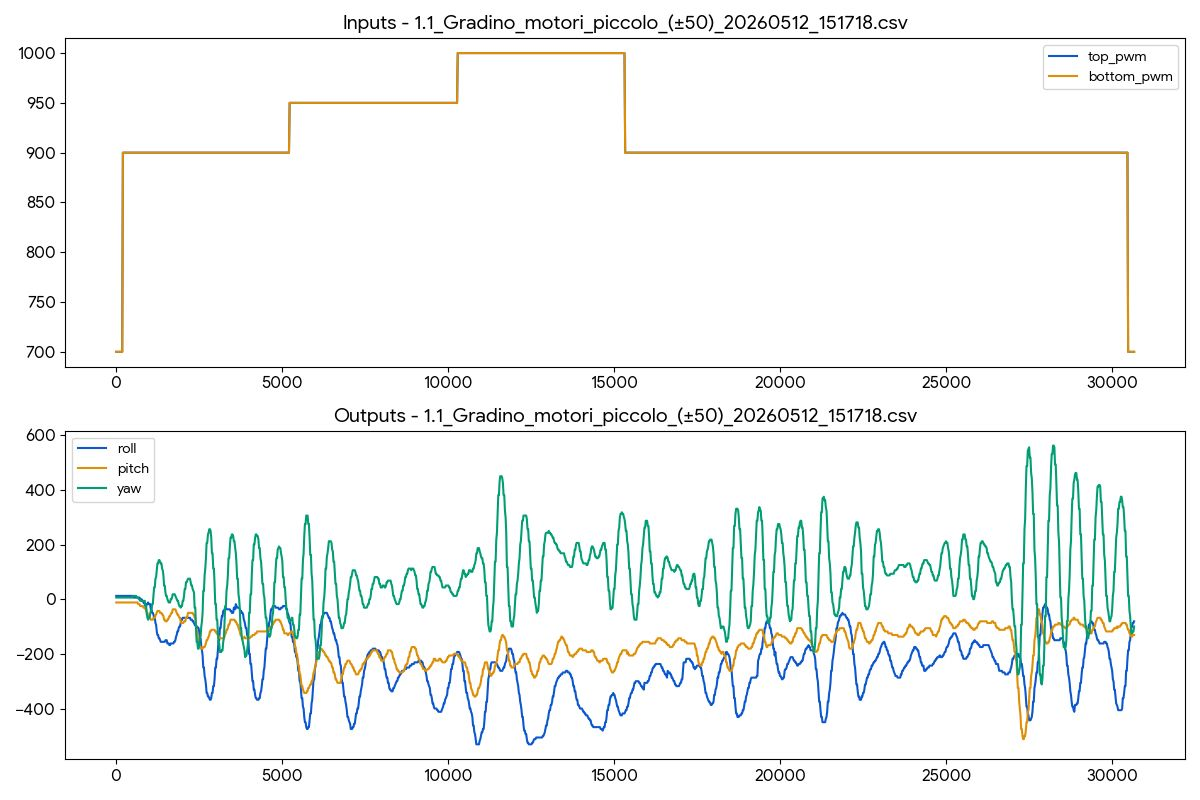
\includegraphics[width=0.88\textwidth]{figures/04_telemetria/test_gradino_motori.png}
		\caption{Esempio di test a gradino in anello aperto (prova 1.1, gradino motori piccolo $\pm 50$): comandi PWM ai motori e ai servo, e risposta angolare del drone}
		\label{fig:test_gradino_motori}
	\end{figure}
	
	\subsection{Segnali armonici e chirp}
	Le prove armoniche (ad esempio 3.4, 3.5, 4.4, 4.5) comandano i \textit{flap} affinché oscillino con una frequenza specifica (tipicamente 0.5 [Hz] o 2.0 [Hz]). Le prove \textit{chirp} (3.6, 4.6) impongono invece una frequenza spazzolata linearmente tra 0.1 e 3 [Hz] nell'arco della durata della prova.
	
	Questi segnali permettono di tracciare empiricamente il diagramma di Bode del sistema: all'aumentare della frequenza di oscillazione del comando, l'inerzia del velivolo ne attenua progressivamente l'ampiezza di risposta e ne introduce uno sfasamento. Il \textit{chirp} è particolarmente prezioso perché, in un'unica prova, copre un'intera decade di frequenze e consente di individuare eventuali frequenze di risonanza del telaio in PLA o del sistema elastico delle funi, informazione utile in fase successiva qualora si rendesse necessario inserire filtri \textit{notch} o passa-basso nei rami di retroazione.
	
	\subsection{Sequenze pseudo-casuali multilivello}
	\label{subsec:aprbs}
	Le prove contrassegnate dai codici 5.2, 5.3 e 5.4 implementano sequenze pseudo-casuali multilivello, riconducibili alla famiglia delle \textit{Amplitude-modulated Pseudo-Random Binary Sequences} (APRBS). A differenza della PRBS classica --- generata da un \textit{Linear Feedback Shift Register} e limitata a due livelli di ampiezza --- l'APRBS impiegata in questo lavoro adotta cinque livelli discreti di ampiezza, mantenendo invariata la natura pseudo-casuale dei salti. Per coerenza con la nomenclatura adottata nello \textit{script} di acquisizione e nei nomi dei \textit{dataset} prodotti, nel seguito si continuerà a indicare queste sequenze con la sigla \textit{PRBS}, fermo restando che la definizione tecnicamente più corretta è quella di sequenza multilivello.
	
	In queste modalità il comando inviato ai \textit{flap} non segue una legge matematica continua, ma salta in modo istantaneo tra livelli discreti definiti a partire dalle costanti \texttt{STEP\_SMALL} e \texttt{STEP\_MEDIUM}, a intervalli temporali regolari (ogni 0.5 [s]).
	
	Le sequenze pseudo-casuali rappresentano uno standard nell'identificazione \textit{black-box} dei sistemi dinamici. Da un punto di vista spettrale, un salto pseudo-casuale tra livelli discreti approssima il comportamento di un rumore bianco entro la banda di interesse: il segnale contiene energia su un'ampia gamma di frequenze, permettendo di stimolare contemporaneamente tutti i modi della dinamica e di alimentare in modo efficiente gli algoritmi di identificazione parametrica come \texttt{tfest} (descritto nel Capitolo~\ref{ch:modello}). Va tuttavia osservato che la scelta di cinque livelli (incluso lo zero) anziché due livelli puri --- come prescriverebbe la PRBS classica --- comporta una lieve riduzione dell'energia spettrale totale a parità di ampiezza massima, in quanto durante i blocchi in cui il livello selezionato è zero il sistema non viene effettivamente eccitato. Questa scelta è stata ritenuta accettabile in quanto rende il segnale meccanicamente meno aggressivo sui servomotori e sulle funi, prolungandone la vita utile durante le ripetute campagne di acquisizione.
	
	Le prove 5.2 (PRBS \textit{roll}) e 5.3 (PRBS \textit{pitch}) hanno svolto il ruolo principale nella stima delle funzioni di trasferimento $G_\text{roll}(z)$ e $G_\text{pitch}(z)$ presentate nel prossimo capitolo. La scelta è motivata da due proprietà del segnale.
	\begin{itemize}
		\item \textbf{Copertura spettrale ampia}: poiché la sequenza di livelli e la direzione dei salti variano in modo stocastico, pur rimanendo ancorate al passo di 0.5 [s], il segnale presenta energia significativa sia alle basse frequenze (quando il livello rimane costante per più blocchi consecutivi) sia alle alte frequenze (quando il livello cambia ad ogni blocco).
		\item \textbf{Stimolazione di transitori e regime}: il sistema viene costretto a eseguire continui transitori intervallati da brevi finestre di assestamento, permettendo all'algoritmo di identificazione di catturare sia gli effetti inerziali sia il comportamento di regime nelle vicinanze dell'equilibrio.
	\end{itemize}
	L'implementazione della modalità 5.2 (PRBS \textit{roll}) è riportata di seguito:
	
	\begin{lstlisting}[language=Matlab, caption={Generazione della sequenza pseudo-casuale multilivello sul flap di roll (case 21)}]
case 21
    % 5.2 PRBS roll ogni 0.5 s
    block = floor(time / 0.5);
    rng(block);
    levels = [-MEDIUM, -SMALL, 0, SMALL, MEDIUM];
    idx = randi(numel(levels));
    roll = CENTER + levels(idx);
	\end{lstlisting}
	
	Il funzionamento si articola in tre passi.
	\begin{enumerate}
		\item L'istruzione \texttt{block = floor(time / 0.5)} divide la durata della prova in finestre temporali discrete di mezzo secondo, e associa a ciascuna finestra un indice intero.
		\item L'istruzione \texttt{rng(block)} reimposta il \textit{seed} del generatore casuale di MATLAB all'inizio di ogni blocco. Questo dettaglio è cruciale: garantisce che, anche ripetendo lo stesso test in giorni diversi, la sequenza di salti casuali estratta sia esattamente la stessa. La ripetibilità della sollecitazione è una condizione necessaria per confrontare i dati di telemetria reali con le uscite del simulatore a parità di ingresso.
		\item Infine, la funzione \texttt{randi} seleziona in modo equiprobabile uno dei cinque livelli discreti $\{-100, -50, 0, +50, +100\}$ in unità CCR, che viene sommato al valore neutro \texttt{CENTER\_SERVO} per ottenere il comando finale al servomotore di \textit{roll}.
	\end{enumerate}
	La prova 5.3 (PRBS \textit{pitch}) ha struttura identica, applicata al servomotore di \textit{pitch}. La prova 5.4 combina le due sequenze sui due assi simultaneamente, con \textit{seed} indipendenti per garantire la decorrelazione fra i due ingressi.
	
	\subsection{Eccitazioni multi-asse}
	Le modalità finali dello \textit{script} (prova 5.1 \textit{roll}+\textit{pitch} alternati, e prova 5.4 PRBS combinata) stimolano contemporaneamente o in modo alternato entrambi gli assi geometrici del velivolo. Questi test sono particolarmente utili per evidenziare gli effetti di accoppiamento dinamico (\textit{cross-coupling}) tra \textit{roll} e \textit{pitch}, dovuti alla geometria interna del condotto, all'effetto giroscopico delle eliche e all'eventuale deviazione asimmetrica del flusso d'aria. Mentre le prove monoasse permettono di identificare modelli SISO per ciascun ramo, le prove multi-asse forniscono il dato necessario per costruire eventuali modelli MIMO più completi nelle estensioni future del progetto.
	
	%--------------------------------------------------------------
	\section{Validazione del link telematico}
	\label{sec:validazione_link}
	
	Al termine di ogni prova, lo \textit{script} produce un \textit{report} riassuntivo che costituisce la metrica con cui validare la qualità della singola acquisizione:
	
	\begin{lstlisting}[language=Matlab, caption={Esempio di report di fine prova}]
fprintf("\n========== REPORT FINALE ==========\n");
fprintf("File CSV: %s\n", filename);
fprintf("Motivo stop: %s\n", STOP_REASON);
fprintf("Righe telemetria salvate: %d\n", stats.telemetryRows);
fprintf("ACK_ERR ricevuti:  %d\n", stats.ackErr);
fprintf("Righe corrotte/vuote ignorate: %d\n", stats.badLines);
fprintf("===================================\n");
	\end{lstlisting}
	
	I tre indicatori principali del \textit{report} sono:
	\begin{itemize}
		\item \texttt{telemetryRows} --- numero totale di righe CSV salvate sul file. In una prova di 30 [s] a 50 [Hz] il valore atteso è prossimo a 1500;
		\item \texttt{badLines} --- numero di righe ricevute ma scartate dal parsing per non aver superato il controllo delle 14 virgole. Un valore non nullo segnala disturbi sul canale o un \textit{baudrate} prossimo al limite di saturazione;
		\item \texttt{ackErr} --- numero di risposte \texttt{ACK\_ERR} ricevute dal firmware, indicative di comandi malformati lato MATLAB.
	\end{itemize}
	
	Nelle campagne sperimentali svolte, i \textit{dataset} effettivamente utilizzati per la successiva fase di identificazione sono stati prevalentemente quelli generati dalle prove PRBS sui due assi di assetto. In particolare, il \textit{dataset} \texttt{5.3\_PRBS\_pitch\_*.csv} contiene oltre 1500 campioni utili con motori accesi, mentre il \textit{dataset} \texttt{5.2\_PRBS\_roll\_*.csv} contiene circa 840 campioni utili --- in entrambi i casi sufficienti, per durata e ricchezza spettrale, ad alimentare in modo efficace gli algoritmi di \texttt{tfest} descritti nel Capitolo~\ref{ch:modello}.
	
	Con la produzione di questi file \texttt{.csv} il sistema è pronto per la fase successiva, in cui i dati registrati vengono elaborati in MATLAB per l'identificazione delle funzioni di trasferimento del velivolo e per la sintesi dei regolatori PID.

    %%%%%%%%%%%%%%%%%%%%%%%%%%%%%%%%%%%%%%%%%%%%%%%%%%%%%%%%%%%%%%%%%%%%
	%             CAPITOLO 5 - IDENTIFICAZIONE DEL MODELLO
	%%%%%%%%%%%%%%%%%%%%%%%%%%%%%%%%%%%%%%%%%%%%%%%%%%%%%%%%%%%%%%%%%%%%
	\chapter{Identificazione del modello}
	\label{ch:modello}
	
	Il presente capitolo descrive la fase di costruzione del modello matematico del \textit{Double Propeller Ducted-Fan (DPDF)} e la successiva sintesi dei regolatori PID. La procedura adottata è di tipo \textit{data-driven}: il modello dinamico del velivolo non viene derivato analiticamente dalle equazioni della meccanica, bensì \textit{stimato} a partire dai \textit{dataset} di telemetria acquisiti nel Capitolo~\ref{ch:telemetria}. I modelli identificati vengono poi impiegati per la sintesi automatica dei controllori tramite \texttt{pidtune}, con verifica della risposta in anello chiuso in simulazione prima della validazione sul prototipo fisico.
	
	%--------------------------------------------------------------
	\section{Approccio data-driven}
	\label{sec:approccio_datadriven}
	
	La modellistica analitica classica, basata sulle equazioni cardinali della dinamica di Newton-Eulero, descrive accuratamente il comportamento cinematico di un corpo rigido nello spazio. Nel caso di un velivolo con architettura \textit{DPDF}, tuttavia, tale approccio risulta parziale. Le complesse interazioni fluidodinamiche che si generano all'interno del condotto --- lo strato limite lungo le pareti interne, l'effetto di scia indotto dalle due eliche controrotanti, le mutue interferenze aerodinamiche tra i flussi e i \textit{flap} di controllo --- introducono non-linearità e incertezze parametriche difficilmente quantificabili \textit{a priori}.
	
	Per superare tali limitazioni si è scelto un approccio orientato ai dati, implementando una procedura di identificazione del sistema a \textbf{scatola nera} (\textit{Black-Box Identification}). Questa metodologia permette di ricavare un modello matematico lineare e tempo-invariante (LTI) nell'intorno del punto di lavoro statico, partendo esclusivamente dall'analisi delle risposte temporali del prototipo stimolato in anello aperto.
	
	Vale la pena anticipare che il modello LTI così ottenuto è valido localmente, in un intorno limitato della condizione di equilibrio. Le dinamiche globali del velivolo --- inclusi gli accoppiamenti tra gli assi, gli effetti delle saturazioni meccaniche e l'interazione con il vincolo elastico delle funi --- saranno invece esplorate tramite il simulatore fisico tridimensionale descritto nel Capitolo~\ref{ch:simulazione}, che adotta un modello a parametri concentrati di tipo \textit{grey-box} e complementa le funzioni di trasferimento qui identificate.
	
	%--------------------------------------------------------------
	\section{Pre-elaborazione dei dati}
	\label{sec:pre_elaborazione}
	
	I dati acquisiti dal firmware durante le prove vengono salvati nei file \texttt{.csv} descritti nel Capitolo~\ref{ch:telemetria}. In questi file i comandi impartiti ai servomotori sono espressi in unità CCR (\textit{Capture-Compare Register}), mentre le letture di assetto dell'IMU sono registrate in centesimi di grado.
	
	Prima di procedere alla stima delle funzioni di trasferimento è necessario un processo di conversione e condizionamento dei segnali. L'obiettivo è duplice: convertire le variabili in unità ingegneristiche coerenti (gradi fisici sia per l'ingresso che per l'uscita) e traslare l'origine dei segnali, in modo che rappresentino le pure variazioni dinamiche $\Delta$ rispetto alla condizione di equilibrio statico.
	
	\begin{figure}[H]
		\centering
		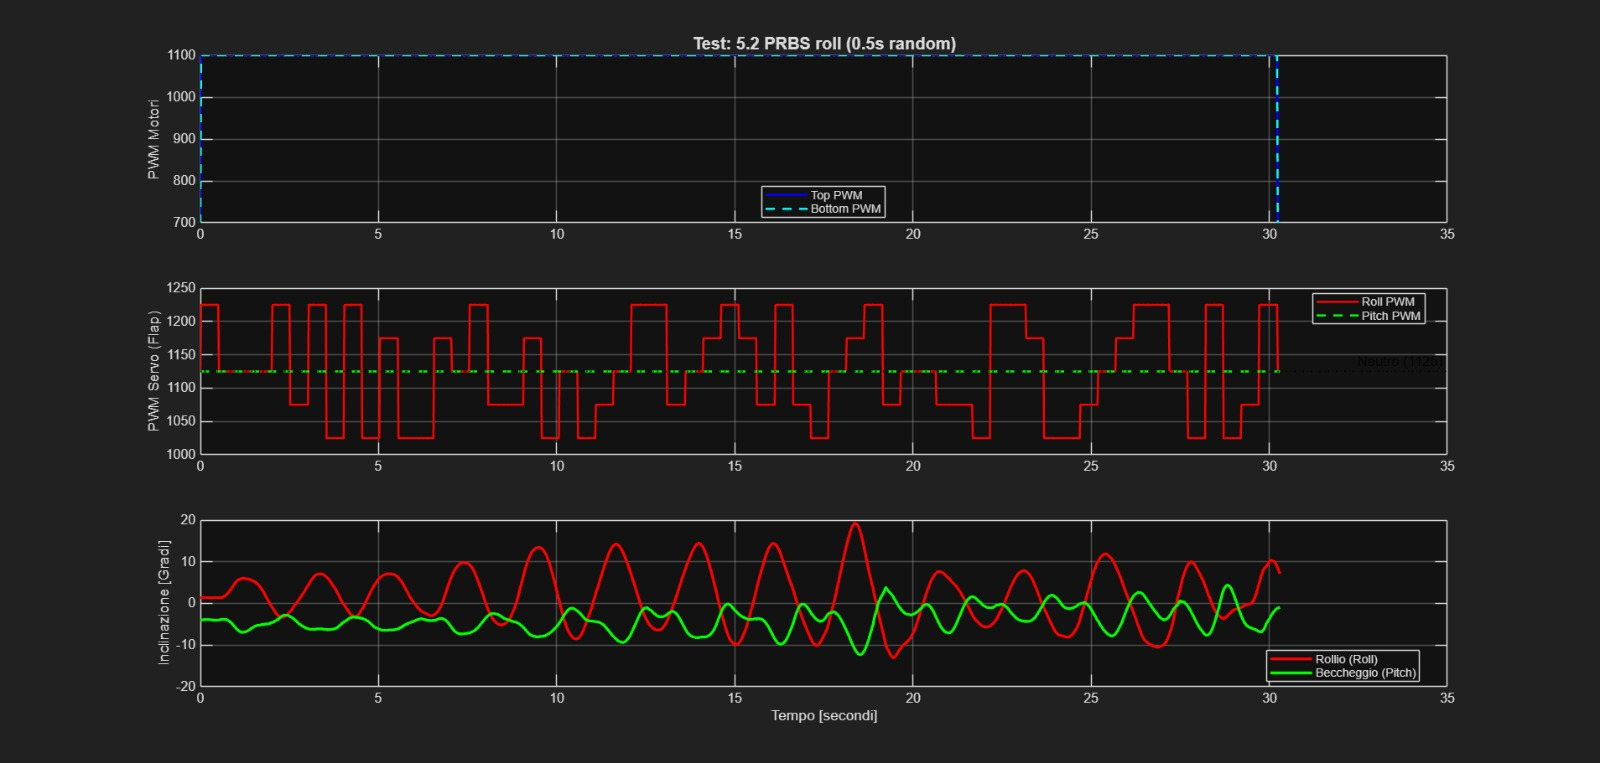
\includegraphics[width=0.75\textwidth]{figures/05_modello/dataset_prbs1.png}
	\end{figure}
	
		\begin{figure}[H]
		\centering
		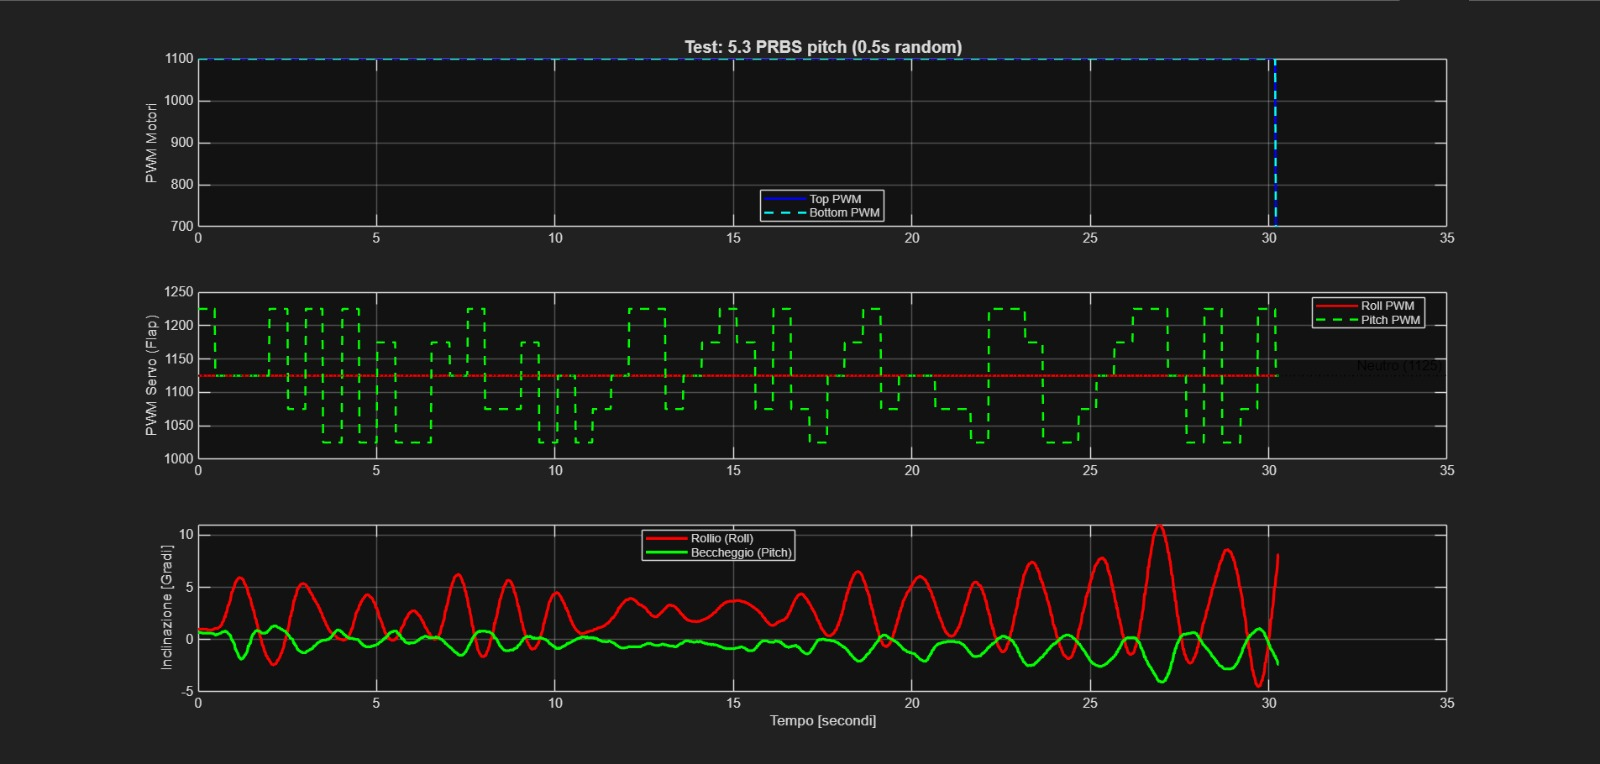
\includegraphics[width=0.75\textwidth]{figures/05_modello/dataset_prbs2.png}
		\caption{\textit{Dataset} sperimentale ad anello aperto ottenuto tramite stimolazione PRBS. In alto: comandi PWM ai motori; al centro: comandi PWM ai \textit{flap}; in basso: risposta angolare del velivolo misurata dall'IMU. A sinistra l'asse di \textit{roll}, a destra l'asse di \textit{pitch}}
		\label{fig:dataset_prbs}
	\end{figure}
	La centratura del segnale d'ingresso rispetto alla posizione neutra del \textit{flap} ($CCR_\text{neutro} = 1125$) è governata dalla relazione:
	\begin{equation}
		\Delta u(t) = \frac{CCR_\text{flap}(t) - CCR_\text{neutro}}{K_\text{CCR}}
		\label{eq:centratura_input}
	\end{equation}
	dove $K_\text{CCR} = 10.0$ [CCR/deg] rappresenta la costante di conversione statica del servomotore \textit{Hitec HS-82MG} adottato.
	
	Analogamente, la misura dell'angolo di assetto $\theta(t)$ (\textit{roll} o \textit{pitch}) viene convertita in gradi e depurata dal valore medio di \textit{offset} $\bar\theta$ registrato durante la fase di equilibrio:
	\begin{equation}
		\Delta y(t) = \frac{\theta_\text{cdeg}(t)}{100} - \bar\theta
		\label{eq:centratura_output}
	\end{equation}
	
	L'implementazione di questa fase di pre-elaborazione è riportata nel codice MATLAB seguente:
	
	\begin{lstlisting}[language=Matlab, caption={Pre-elaborazione dei segnali di ingresso e uscita}]
CCR_PER_DEGREE = 10.0;   % Costante di conversione servo
CENTER_SERVO   = 1125;   % Zero meccanico flap

% Condizionamento dell'ingresso (comando flap in gradi)
u_raw      = double(T_asse.roll_pwm);   % o pitch_pwm secondo l'asse
u_centered = (u_raw - CENTER_SERVO) / CCR_PER_DEGREE;

% Condizionamento dell'uscita (angolo IMU in gradi)
y_raw      = double(T_asse.roll_cdeg) / 100.0;
y_mean     = mean(y_raw);
y_centered = y_raw - y_mean;

% Creazione dell'oggetto iddata per il System Identification Toolbox
Ts         = 0.02;       % Periodo di campionamento (50 Hz)
data_ident = iddata(y_centered, u_centered, Ts);
	\end{lstlisting}
	
	Il periodo di campionamento $T_s = 0.02$ [s] coincide con la frequenza di trasmissione della telemetria (50 [Hz]) ed è coerente con la frequenza alla quale il PID, una volta validato, opererà nel firmware. Questa scelta evita disallineamenti tra il modello identificato e l'ambiente in cui i regolatori saranno effettivamente eseguiti.
	
	%--------------------------------------------------------------
	\section{Selezione dell'architettura del modello}
	\label{sec:architettura_modello}
	
	Per identificare la dinamica del sistema SISO (\textit{Single-Input Single-Output}) che lega lo spostamento angolare dei \textit{flap} alla rotazione del velivolo attorno ai rispettivi assi principali, si è utilizzato il \textit{System Identification Toolbox} di MATLAB, in particolare la funzione \texttt{tfest}. La stima è stata condotta nel dominio del tempo continuo, configurando l'algoritmo iterativo di ottimizzazione su una struttura a tempo continuo che viene poi convertita a tempo discreto per il confronto con i dati.
	
	Per evitare fenomeni di sovra-parametrizzazione del rumore di misura ad alta frequenza (causato principalmente dalle vibrazioni dei motori \textit{brushless}), la complessità strutturale della funzione di trasferimento è stata limitata sulla base di considerazioni fisiche. La dinamica complessiva del drone può essere approssimata, in prima istanza, a un sistema del secondo ordine --- caratterizzato da un comportamento inerziale e da uno smorzamento aerodinamico --- a cui si aggiungono il ritardo di attuazione dei servomotori e l'effetto di un eventuale zero al numeratore.
	
	La struttura generale del modello LTI a tempo continuo che si cerca di identificare è:
	\begin{equation}
		G(s) = \frac{\Delta Y(s)}{\Delta U(s)} = \frac{b_m s^m + \dots + b_1 s + b_0}{s^n + a_{n-1} s^{n-1} + \dots + a_1 s + a_0}
		\label{eq:tf_generale}
	\end{equation}
	
	Sono state confrontate tre strutture candidate per ciascun asse: \textbf{2 poli e 1 zero}, \textbf{2 poli e 0 zeri}, \textbf{3 poli e 1 zero}. L'analisi iterativa condotta sui \textit{dataset} PRBS ha evidenziato due architetture ottimali per i rispettivi assi:
	\begin{itemize}
		\item \textbf{Asse di \textit{roll}}: modello a 2 poli e 1 zero ($n=2$, $m=1$), che cattura adeguatamente la dinamica inerziale del velivolo nella sezione trasversale.
		\item \textbf{Asse di \textit{pitch}}: modello a 3 poli e 1 zero ($n=3$, $m=1$). Il polo aggiuntivo rispetto all'asse di \textit{roll} è imputabile alla maggiore complessità del flusso aerodinamico in direzione longitudinale, dovuta alla configurazione asimmetrica dei due rotori in cascata.
	\end{itemize}
	
	Le rispettive funzioni di trasferimento hanno dunque forma:
	\begin{equation}
		G_\text{roll}(s) = \frac{b_1 s + b_0}{s^2 + a_1 s + a_0},
		\qquad
		G_\text{pitch}(s) = \frac{b_1 s + b_0}{s^3 + a_2 s^2 + a_1 s + a_0}
		\label{eq:tf_assi}
	\end{equation}
	
	I valori numerici dei coefficienti $a_i$ e $b_j$ ottenuti dall'identificazione su \textit{dataset} PRBS sono riportati nella Tabella~\ref{tab:coefficienti_tf}.
	
	\begin{table}[H]
		\centering
		\begin{tabular}{l c c}
			\toprule
			\textbf{Coefficiente} & \textbf{$G_\text{roll}(s)$ (2p, 1z)} & \textbf{$G_\text{pitch}(s)$ (3p, 1z)} \\
			\midrule
			$b_1$ & --- (da inserire) & --- (da inserire) \\
			$b_0$ & --- (da inserire) & --- (da inserire) \\
			$a_2$ & --- (n/a)         & --- (da inserire) \\
			$a_1$ & --- (da inserire) & --- (da inserire) \\
			$a_0$ & --- (da inserire) & --- (da inserire) \\
			\bottomrule
		\end{tabular}
		\caption{Coefficienti numerici delle funzioni di trasferimento identificate. I valori vanno inseriti a partire dall'output dello script \texttt{Identify\_and\_tune.m}}
		\label{tab:coefficienti_tf}
	\end{table}
	
	%--------------------------------------------------------------
	\section{Stima del modello e validazione}
	\label{sec:stima_validazione}
	
	La stima dei coefficienti è stata effettuata tramite la funzione \texttt{tfest} del \textit{System Identification Toolbox}, configurata per imporre la stabilità del modello stimato (opzione \texttt{EnforceStability}). Lo \textit{script} di identificazione \texttt{Identify\_and\_tune.m} confronta automaticamente le tre strutture candidate e seleziona quella con il \textit{fit} più elevato:
	
	\begin{lstlisting}[language=Matlab, caption={Confronto automatico delle tre strutture candidate (estratto da \texttt{Identify\_and\_tune.m})}]
opt_tf = tfestOptions('EnforceStability', true, 'Display', 'off');

% Modello A: 2 poli, 1 zero
sysA = tfest(data_ident, 2, 1, opt_tf);
fitA = goodnessOfFit(sim(sysA, data_ident).y, y_centered, 'NRMSE') * 100;

% Modello B: 2 poli, 0 zeri
sysB = tfest(data_ident, 2, 0, opt_tf);
fitB = goodnessOfFit(sim(sysB, data_ident).y, y_centered, 'NRMSE') * 100;

% Modello C: 3 poli, 1 zero
sysC = tfest(data_ident, 3, 1, opt_tf);
fitC = goodnessOfFit(sim(sysC, data_ident).y, y_centered, 'NRMSE') * 100;

[best_fit, best_idx] = max([fitA, fitB, fitC]);
	\end{lstlisting}
	
	La bontà del modello identificato è valutata mediante l'indice di \textit{fit} percentuale basato sulla NRMSE (\textit{Normalized Root Mean Square Error}):
	\begin{equation}
		\text{Fit} = 100 \cdot \left( 1 - \frac{\sqrt{\sum_{k=1}^{N} \bigl| y(k) - \hat y(k) \bigr|^{2}}}{\sqrt{\sum_{k=1}^{N} \bigl| y(k) - \bar y \bigr|^{2}}} \right) \quad [\%]
		\label{eq:nrmse}
	\end{equation}
	dove $y(k)$ è la misura sperimentale dell'IMU, $\hat y(k)$ è la risposta temporale simulata dal modello identificato e $\bar y$ è il valore medio del segnale reale. Un valore del 100\% indica una corrispondenza perfetta; un valore prossimo a 0\% indica che il modello non spiega la varianza del dato meglio di una semplice media costante.
	
	I valori di \textit{fit} ottenuti sui \textit{dataset} PRBS sono:
	\begin{itemize}
		\item Asse di \textit{roll}: $\text{Fit} = 77.85\%$
		\item Asse di \textit{pitch}: $\text{Fit} = 77.67\%$
	\end{itemize}
	
	Si tratta di valori soddisfacenti per un'identificazione \textit{black-box} su un sistema dotato di non-linearità importanti e condizioni di prova vincolate. La quota residua di varianza non spiegata dal modello è imputabile a effetti che il modello LTI non può catturare: in particolare l'attrito non lineare sui perni dei \textit{flap}, l'azione non perfettamente simmetrica delle funi di vincolo e i piccoli accoppiamenti tra gli assi non separabili dal modello SISO.
	
	\begin{figure}[H]
		\centering
		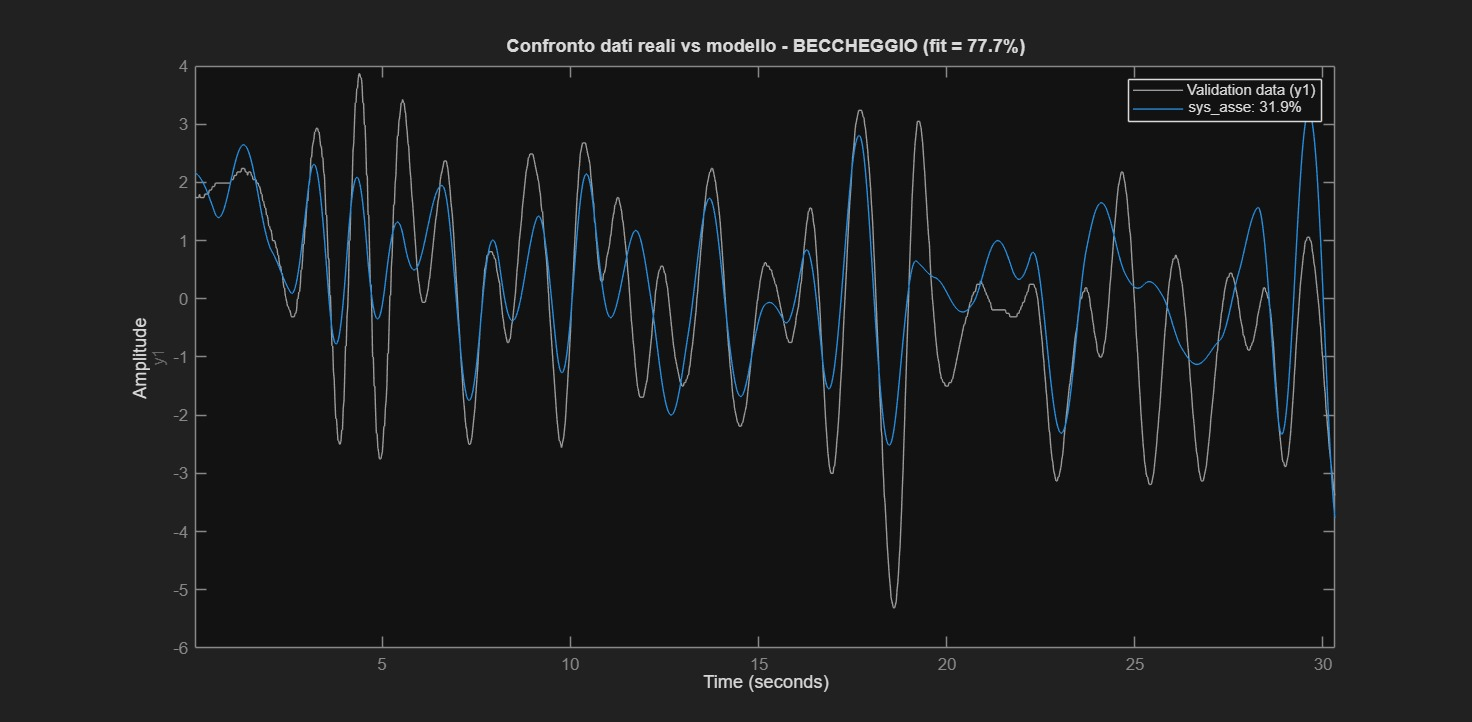
\includegraphics[width=0.95\textwidth]{figures/05_modello/cross_validation1.png}
	\end{figure}
	
		\begin{figure}[H]
		\centering
		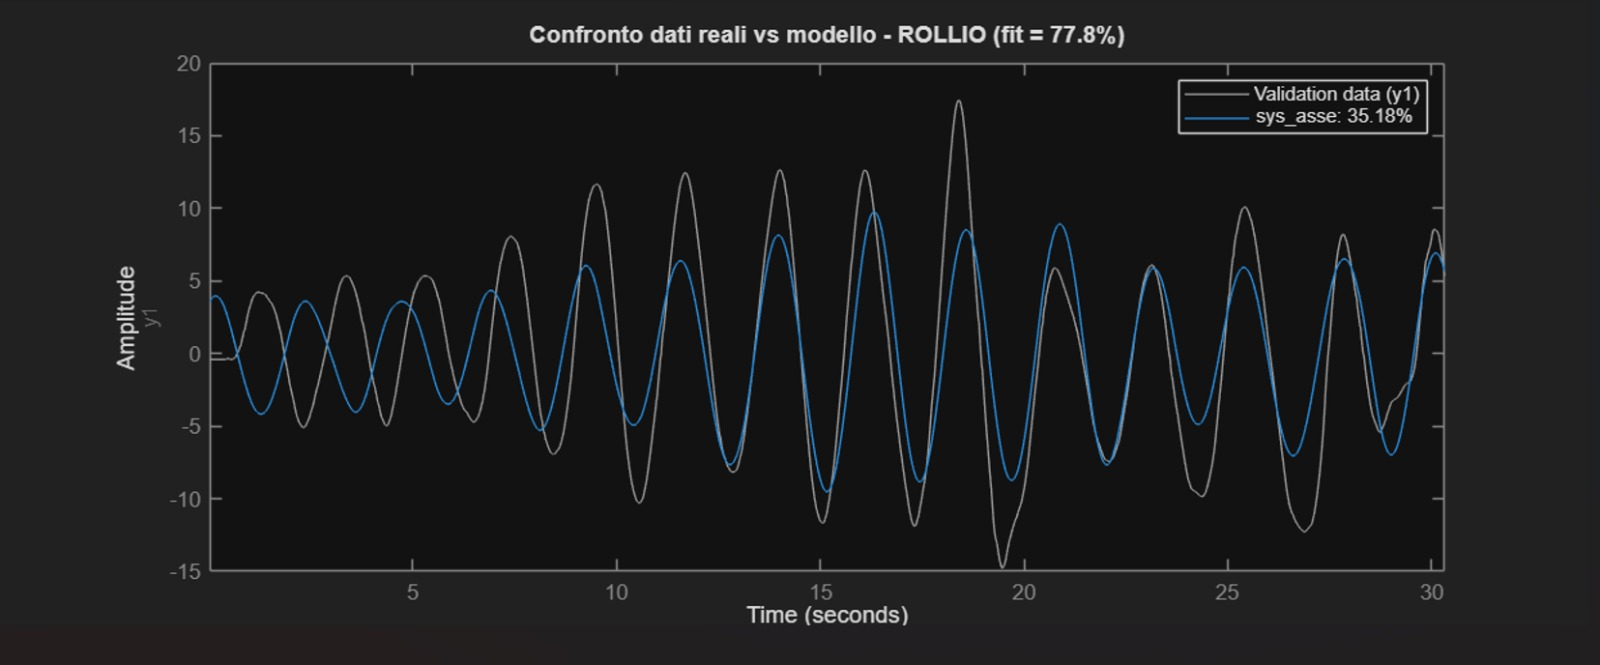
\includegraphics[width=0.95\textwidth]{figures/05_modello/cross_validation2.png}
		\caption{Analisi di \textit{cross-validazione} nel dominio del tempo per i due assi. Confronto tra risposta angolare reale del prototipo (linea nera) e uscita stimata dal modello LTI (linea colorata). A sinistra l'asse di \textit{roll} (Fit $77.85\%$), a destra l'asse di \textit{pitch} (Fit $77.67\%$)}
		\label{fig:cross_validation}
	\end{figure}
	
	\subsection{Analisi del guadagno statico}
	Un'analisi che permette di validare fisicamente il modello identificato riguarda l'estrazione del guadagno statico del sistema, calcolato applicando il teorema del valore finale per $s \to 0$:
	\begin{equation}
		\mu = \lim_{s \to 0} G(s) = \frac{b_0}{a_0}
		\label{eq:guadagno_statico}
	\end{equation}
	I test condotti hanno restituito, per entrambi gli assi, un guadagno statico di \textbf{segno negativo} ($\mu < 0$). Questo risultato fornisce una conferma fisica del modello stimato: un incremento del PWM del servomotore --- corrispondente a un'inclinazione positiva del \textit{flap} secondo la convenzione del firmware --- genera una coppia aerodinamica che ruota il drone nel verso opposto rispetto al sistema di riferimento destrorso solidale all'IMU. Tale inversione di segno, conseguenza della geometria meccanica del prototipo, vincolerà la successiva sintesi del controllore e la sua integrazione nel \textit{mixer} di controllo del firmware.
	
	%--------------------------------------------------------------
	\section{Sintesi del controllore PIDF}
	\label{sec:sintesi_pidf}
	
	Identificato il modello matematico $G(s)$ del processo, si è proceduto alla sintesi dell'algoritmo di controllo ad anello chiuso. L'architettura scelta è un controllore PID in forma parallela con l'azione derivativa asservita a un filtro passa-basso del primo ordine, configurazione comunemente indicata come \textbf{PIDF}.
	
	\subsection{Architettura del controllore}
	La presenza del filtro derivativo, caratterizzato dalla costante di tempo $T_f$, è indispensabile per limitare l'amplificazione del rumore di misura alle alte frequenze: senza filtraggio, la derivata pura del rumore del BNO-055 produrrebbe comandi ad alta ampiezza e alta frequenza ai servomotori, con conseguente fenomeno di \textit{chattering} (vibrazioni rapide e meccanicamente dannose). La funzione di trasferimento del controllore nel dominio di Laplace ha forma:
	\begin{equation}
		C(s) = K_p + \frac{K_i}{s} + \frac{K_d \, s}{T_f \, s + 1}
		\label{eq:pidf}
	\end{equation}
	
	\subsection{Sintesi tramite pidtune}
	Il calcolo dei guadagni ottimali è stato effettuato tramite l'algoritmo di ottimizzazione \texttt{pidtune} di MATLAB. Per mitigare i rischi di danneggiamento meccanico durante le prime prove sul prototipo, i vincoli di progetto sono stati impostati in modo conservativo:
	\begin{enumerate}
		\item Il parametro \texttt{DesignFocus} è stato configurato su \texttt{'reference-tracking'} per privilegiare la dolcezza di inseguimento del riferimento ed eliminare sovraelongazioni pronunciate; tale impostazione produce guadagni più contenuti rispetto all'alternativa \texttt{'disturbance-rejection'}, più aggressiva ma anche più rischiosa per un primo collaudo.
		\item L'azione di controllo $u_\text{ctrl}(t)$ è stata costantemente monitorata in simulazione per garantire il rispetto del vincolo di saturazione fisica dei \textit{flap}, fissato a $\pm 30\degree$:
		\begin{equation}
			\max \, \bigl| u_\text{ctrl}(t) \bigr| \leq 30\degree
			\label{eq:vincolo_saturazione}
		\end{equation}
	\end{enumerate}
	
	\begin{lstlisting}[language=Matlab, caption={Sintesi del controllore PIDF con pidtune}]
pid_opts        = pidtuneOptions('DesignFocus', 'reference-tracking');
[C_pid, info]   = pidtune(sys_asse, 'PIDF', pid_opts);

% Verifica in anello chiuso e azione di controllo
sys_cl   = feedback(C_pid * sys_asse, 1);    % risposta a gradino
sys_ctrl = feedback(C_pid, sys_asse);        % sforzo di controllo
	\end{lstlisting}
	
		\begin{figure}[H]
		\centering
		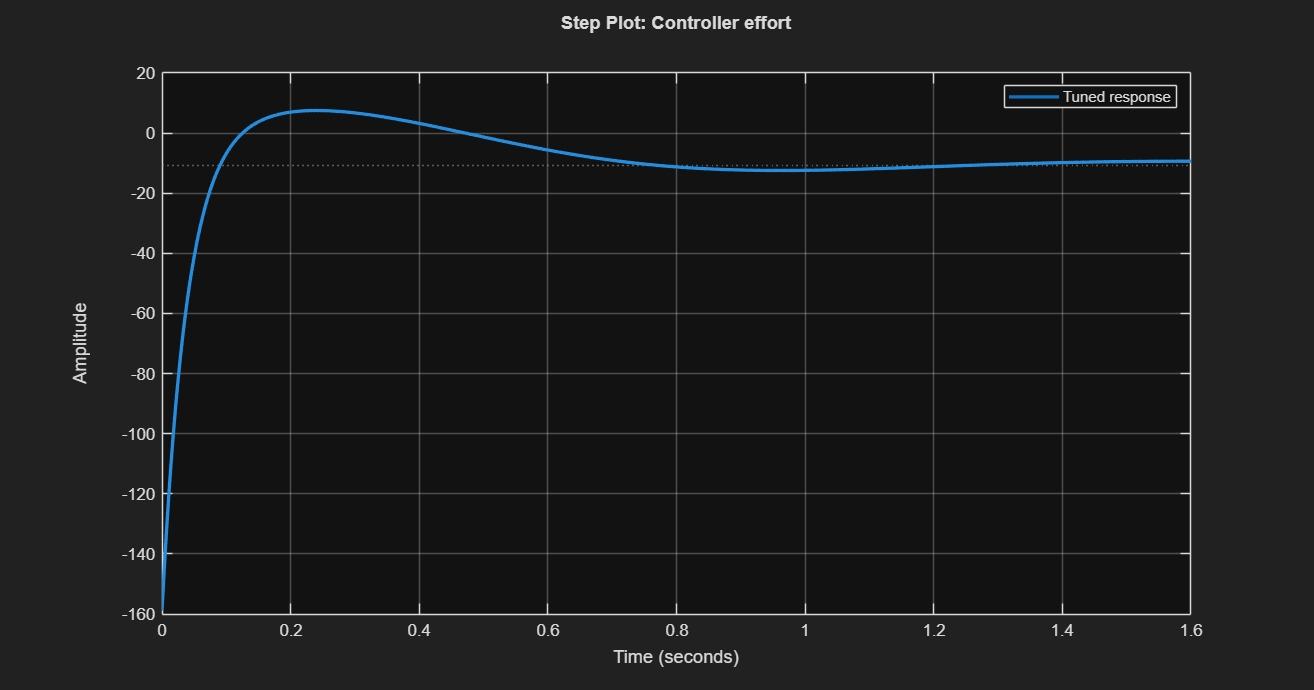
\includegraphics[width=0.95\textwidth]{figures/05_modello/step_response1.png}
	\end{figure}
	
	\begin{figure}[H]
		\centering
		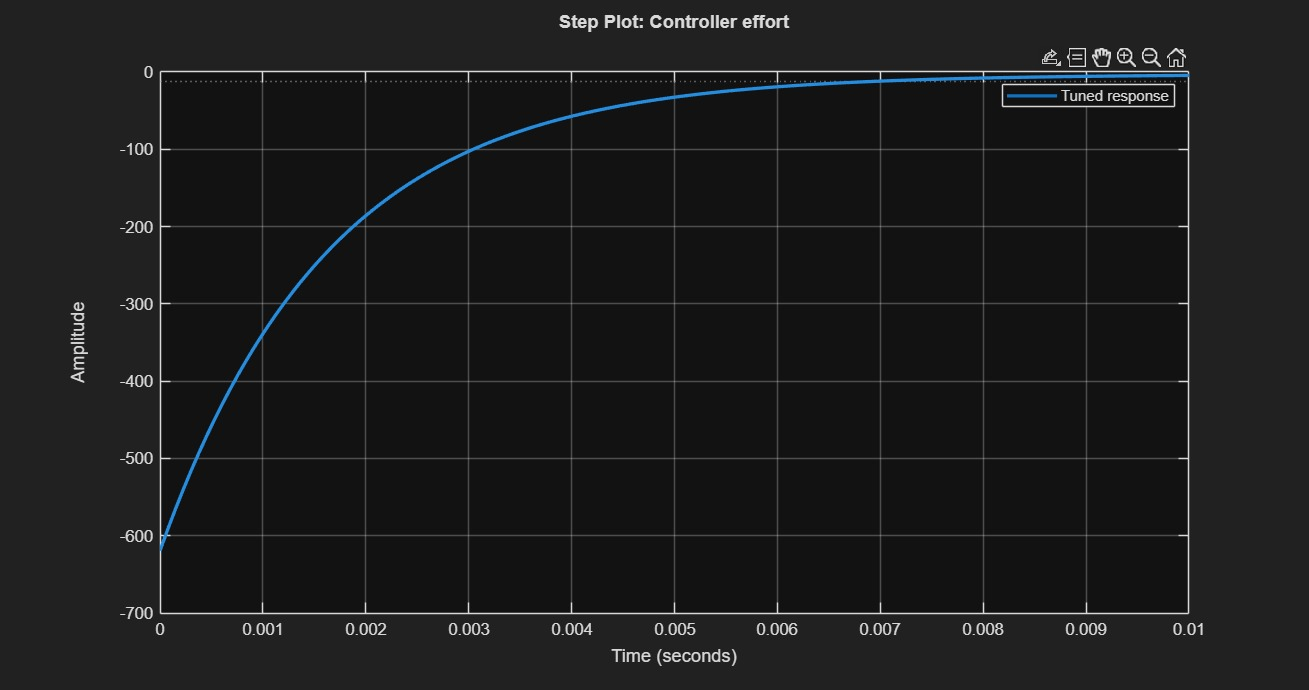
\includegraphics[width=0.95\textwidth]{figures/05_modello/step_response2.png}
		\caption{Analisi della risposta al gradino ad anello chiuso (sinistra) e del corrispondente sforzo di controllo dei servomotori (destra). Il picco iniziale dell'azione di controllo si attesta entro il vincolo fisico di $\pm 30\degree$}
		\label{fig:step_response}
	\end{figure}
	
	Una nota implementativa importante riguarda la \textbf{convenzione di segno} adottata. Il modello identificato presenta guadagno statico negativo ($\mu < 0$, come discusso nella Sezione~\ref{sec:stima_validazione}). Tuttavia, nel codice sorgente del firmware i guadagni $K_p$, $K_i$, $K_d$ vengono inseriti come valori \textbf{positivi}: l'inversione di segno necessaria per produrre un momento correttivo opposto al disturbo viene gestita a valle, all'interno della logica di \textit{mixer} che combina l'uscita del PID con il comando applicato al servomotore. Questa scelta separa la legge di controllo \textit{matematica} dalla \textit{convenzione di segno} dell'attuatore meccanico, semplificando la lettura del codice firmware.
	
	\subsection{Discretizzazione per il firmware}
	Il firmware esegue il \textit{loop} di controllo all'interno di un \textit{interrupt} deterministico generato dal \textit{Timer 7} alla frequenza di 50 [Hz], corrispondente a un periodo di campionamento $T_s = 0.02$ [s]. Per mappare la costante di tempo continua del filtro $T_f$ nel coefficiente adimensionale discreto $\alpha$ utilizzato nell'equazione alle differenze del firmware, è stata applicata la trasformazione di Eulero all'indietro (\textit{Backward Euler approximation}):
	\begin{equation}
		s \approx \frac{1 - z^{-1}}{T_s}
		\;\;\Longrightarrow\;\;
		\alpha = \frac{T_s}{T_s + T_f}
		\label{eq:euler_backward}
	\end{equation}
	Il coefficiente $\alpha$ è compreso nell'intervallo $[0,1]$ e determina il peso del filtraggio: un valore prossimo a 1 indica un filtraggio leggero (adatto a segnali poco rumorosi), mentre un valore basso indica un'azione di smorzamento più incisiva. Per il caso in esame i due assi richiedono filtraggi differenti, come risulterà dalla Tabella~\ref{tab:guadagni_pid} riportata nella sezione successiva.
	
	%--------------------------------------------------------------
	\section{Guadagni finali e parametri PID}
	\label{sec:guadagni_finali}
	
	I parametri finali, validati in simulazione e pronti per la compilazione nel file \texttt{config.c} del firmware, sono riassunti nella Tabella~\ref{tab:guadagni_pid}.
	
	\begin{table}[H]
		\centering
		\begin{tabular}{l c c}
			\toprule
			\textbf{Parametro} & \textbf{Asse di Roll} & \textbf{Asse di Pitch} \\
			\midrule
			Modello di partenza        & 2 poli, 1 zero & 3 poli, 1 zero \\
			Guadagno proporzionale $K_p$ & 16.49 & 10.38 \\
			Guadagno integrale $K_i$     & 43.16 & 11.45 \\
			Guadagno derivativo $K_d$    & 1.24  & 2.32  \\
			Coefficiente filtro discreto $\alpha$ & 0.27 & 0.94 \\
			Saturazione del canale       & $\pm 30\degree$ & $\pm 30\degree$ \\
			\bottomrule
		\end{tabular}
		\caption{Guadagni PIDF identificati per i due assi di controllo}
		\label{tab:guadagni_pid}
	\end{table}
	
	I valori riportati nella Tabella~\ref{tab:guadagni_pid} si interpretano nel modo seguente. I guadagni proporzionali e integrali dell'asse di \textit{roll} sono significativamente più elevati di quelli dell'asse di \textit{pitch}, conseguenza diretta dei rispettivi modelli identificati: l'asse di \textit{roll} presenta un guadagno statico più piccolo in modulo, dunque richiede un'azione di controllo proporzionalmente più \textit{forte} per riportare il velivolo nella condizione di riferimento. Per quanto riguarda i coefficienti del filtro derivativo, il valore $\alpha = 0.27$ per il \textit{roll} indica un filtraggio aggressivo, necessario per attenuare il rumore di assetto presente su quest'asse, mentre $\alpha = 0.94$ per il \textit{pitch} indica un filtraggio appena percettibile, segno di un canale di misura più pulito.
	
	%--------------------------------------------------------------
	\section{Considerazioni sull'approccio black-box}
	\label{sec:limiti_blackbox}
	
	I modelli identificati nel presente capitolo forniscono una descrizione lineare e tempo-invariante della risposta angolare del velivolo, valida \textit{localmente} attorno alla condizione di equilibrio. Questa rappresentazione è perfettamente adeguata allo scopo per cui è stata costruita --- la sintesi automatica dei regolatori PID tramite \texttt{pidtune} --- ed è coerente con l'ipotesi di funzionamento del PID stesso, che opera sulla linearizzazione del sistema attorno al riferimento.
	
	Esistono però aspetti della dinamica del \textit{DPDF} che, per loro natura, non possono essere catturati da un modello LTI SISO. Tra questi: l'accoppiamento tra gli assi di \textit{roll} e \textit{pitch}, particolarmente significativo a grandi inclinazioni; gli effetti delle saturazioni meccaniche dei \textit{flap} e degli ESC; l'interazione non lineare tra il velivolo e le quattro funi di vincolo che lo sostengono nella gabbia di sicurezza; e gli effetti geometrici di grande angolo, in cui le proiezioni della spinta sulle componenti orizzontali e verticali cessano di poter essere approssimate dai loro sviluppi al primo ordine.
	
	Per questa ragione, il modello \textit{black-box} qui presentato è stato affiancato da un \textbf{simulatore fisico tridimensionale} a parametri concentrati, descritto nel Capitolo~\ref{ch:simulazione}, che integra le equazioni di Newton-Eulero a 6 gradi di libertà del velivolo e include esplicitamente la geometria, l'accoppiamento tra assi, le saturazioni e il modello elastico delle funi. I due approcci sono complementari e operano su due piani distinti:
	\begin{itemize}
		\item l'\textbf{identificazione \textit{black-box}} (Capitolo~\ref{ch:modello}) produce un modello LTI dedicato alla \textit{sintesi del controllore} con strumenti consolidati come \texttt{pidtune}, e si concentra sul singolo grado di libertà alla volta;
		\item la \textbf{simulazione fisica \textit{grey-box}} (Capitolo 6) fornisce un ambiente di \textit{verifica} in cui i regolatori sintetizzati possono essere testati in condizioni più realistiche, includendo gli effetti non catturati dal modello LTI.
	\end{itemize}
	I due strumenti si chiudono dunque su un percorso unitario: i parametri PID derivati dall'identificazione vengono inseriti nel simulatore per verifica visiva del comportamento complessivo, e solo dopo questa doppia validazione vengono trasferiti al firmware per il collaudo sul prototipo fisico.
	
	Si segnala infine, per completezza, una piccola discrepanza temporale tra i due ambienti: l'identificazione lavora con periodo di campionamento $T_s = 0.02$ [s] coerente con la frequenza del firmware, mentre il simulatore del Capitolo 6 adotta un passo di visualizzazione $\Delta t = 0.025$ [s] suddiviso in più \textit{substep} di integrazione fisica. La scelta è motivata da ragioni di compromesso tra fluidità della visualizzazione 3D e fedeltà numerica dell'integratore, e non altera la validità dei regolatori sintetizzati, che il simulatore continua a eseguire alla loro frequenza nominale.

    %%%%%%%%%%%%%%%%%%%%%%%%%%%%%%%%%%%%%%%%%%%%%%%%%%%%%%%%%%%%%%%%%%%%
	%                CAPITOLO 6 - SIMULAZIONE 3D
	%%%%%%%%%%%%%%%%%%%%%%%%%%%%%%%%%%%%%%%%%%%%%%%%%%%%%%%%%%%%%%%%%%%%
	\chapter{Simulazione 3D}
	\label{ch:simulazione}
	
	La validazione sperimentale di un algoritmo di controllo su un prototipo fisico di velivolo comporta intrinsecamente rischi di instabilità e di danneggiamento dell'hardware, specialmente nelle prime fasi di collaudo. Per mitigare tali rischi e per disporre di un ambiente in cui osservare la dinamica complessiva del sistema in condizioni controllate, si è sviluppato un \textbf{simulatore tridimensionale} in ambiente MATLAB (\texttt{Sim.m}), concepito come un \textit{gemello digitale} del banco di prova di laboratorio.
	
	A differenza dei modelli LTI identificati nel Capitolo~\ref{ch:modello} --- che descrivono la dinamica locale di un singolo asse di assetto attorno al punto di equilibrio --- il simulatore adotta un approccio a parametri concentrati di tipo \textit{grey-box}: integra direttamente le equazioni di Newton-Eulero a 6 gradi di libertà del corpo rigido, include esplicitamente la geometria del prototipo e il modello visco-elastico delle quattro funi di vincolo, e incorpora un modello di spinta calibrato sui dati di telemetria reali. L'obiettivo non è dunque sostituire l'identificazione \textit{black-box} (che resta lo strumento naturale per la sintesi automatica dei regolatori tramite \texttt{pidtune}), ma fornire un ambiente di verifica che includa fenomeni --- accoppiamenti tra assi, momenti ribaltanti, vincolo elastico, saturazioni --- non catturabili da un modello SISO lineare.
	
	%--------------------------------------------------------------
	\section{Obiettivi e architettura del simulatore}
	\label{sec:architettura_sim}
	
	Il simulatore è stato sviluppato con quattro obiettivi principali:
	\begin{enumerate}
		\item \textbf{Verifica dei regolatori PIDF} sintetizzati nel Capitolo~\ref{ch:modello}, in un ambiente che include anche le dinamiche non lineari trascurate dal modello LTI;
		\item \textbf{Comprensione qualitativa} del comportamento del sistema nella configurazione vincolata adottata in laboratorio;
		\item \textbf{Calibrazione iterativa} dei parametri fisici incerti (rigidezza delle funi, smorzamento aerodinamico, autorità dei \textit{flap}) tramite confronto qualitativo con la telemetria sperimentale;
		\item \textbf{De-rating} dei guadagni per il primo collaudo sul prototipo fisico, in modo da disporre di valori conservativi sicuramente stabili.
	\end{enumerate}
	
	\subsection{Architettura a doppio loop temporale}
	Il simulatore implementa l'integrazione numerica delle equazioni del moto mediante un'\textbf{architettura a doppio ciclo temporale}. Il ciclo esterno, gestito da un \texttt{timer} MATLAB, opera alla frequenza macroscopica di visualizzazione e aggiornamento dello stato del controllore, con periodo $\Delta t = 0.025$ [s]. La fisica dei corpi rigidi e delle forze di vincolo viene invece risolta a una frequenza sub-campionata superiore, secondo il metodo dei \textit{sub-stepping} con fattore $N_\text{sub} = 8$, corrispondente a un passo elementare di integrazione $\Delta t_s \approx 0.0031$ [s]. Questa scelta è necessaria per garantire la stabilità numerica dell'integratore esplicito di Eulero impiegato, in particolare in presenza dei coefficienti di rigidezza elevati che caratterizzano il modello delle funi.
	
	Come anticipato nel Capitolo~\ref{ch:modello}, il passo del simulatore ($0.025$ [s]) differisce leggermente dal periodo di campionamento del firmware ($T_s = 0.02$ [s]) per ragioni di compromesso tra fluidità della visualizzazione 3D e fedeltà numerica dell'integrazione: i regolatori vengono comunque eseguiti dal simulatore mantenendo la loro forma discreta, con effetti del tutto trascurabili sulla validità della verifica.
	
	\subsection{Interfaccia interattiva}
	Lo \textit{script} \texttt{Sim.m} include una doppia interfaccia grafica. La finestra principale presenta la scena 3D del drone all'interno della gabbia, con visualizzazione in tempo reale di assetto, traiettoria, tensione delle funi e quota; tre grafici laterali mostrano l'evoluzione temporale di quota, angoli di \textit{roll}/\textit{pitch} e angolo di \textit{yaw}. Una seconda finestra dedicata espone gli \textit{slider} di controllo: due per il CCR dei motori superiore e inferiore (range $[750, 1500]$), sei per i guadagni dei PID di \textit{roll} e \textit{pitch} ($K_p$, $K_i$, $K_d$ per asse), oltre ai pulsanti di START, STOP e RESET. Questa configurazione permette di esplorare interattivamente lo spazio dei parametri, osservando immediatamente l'effetto di ogni modifica sul comportamento del sistema --- modalità di lavoro che si è dimostrata particolarmente efficace durante la fase di calibrazione dei parametri fisici.
	
	%--------------------------------------------------------------
	\section{Parametrizzazione fisica e geometrica}
	\label{sec:parametrizzazione_sim}
	
	Il modello integra i parametri geometrici e inerziali del prototipo, derivati dal modello CAD del \textit{DPDF} e verificati sperimentalmente:
	\begin{itemize}
		\item \textbf{Massa totale del velivolo}: $M = 2.2$ [kg];
		\item \textbf{Matrice di inerzia (diagonale)}: $I_{xx} = 0.0062$ [kg$\cdot$m$^2$], $I_{yy} = 0.0062$ [kg$\cdot$m$^2$], $I_{zz} = 0.0100$ [kg$\cdot$m$^2$];
		\item \textbf{Eccentricità statica del centro di massa} rispetto all'asse geometrico, causata dalle tolleranze di montaggio: $d_{cg,x} = 0.0028$ [m], $d_{cg,y} = 0.0038$ [m];
		\item \textbf{Geometria del cilindro}: altezza $H = 220$ [mm], raggio esterno $R_\text{ext} = 117.5$ [mm];
		\item \textbf{Geometria della gabbia di vincolo}: cubo di lato $3 \cdot H = 660$ [mm] con quattro funi ai vertici superiori, ancorate al bordo inferiore del drone in corrispondenza degli angoli a $45\degree$, $135\degree$, $225\degree$, $315\degree$.
	\end{itemize}
	
	Tutti questi parametri sono raccolti nella \textit{struct} di configurazione \texttt{C}, costruita una sola volta all'avvio del simulatore e successivamente passata per riferimento alle funzioni di integrazione fisica. La medesima \textit{struct} contiene anche le costanti elettriche del sistema propulsivo (tensione batteria, coefficiente di spinta dell'elica, costante motore $K_V$), utilizzate dal modello di spinta descritto nella Sezione~\ref{sec:modello_spinta_flap}.
	
	%--------------------------------------------------------------
	\section{Modello dinamico del corpo rigido}
	\label{sec:dinamica_sim}
	
	La rotazione del velivolo attorno agli assi di rollio ($x$) e beccheggio ($y$) è governata dalle equazioni della dinamica rotazionale in terna solidale, accoppiate alle non-linearità dovute all'eccentricità del baricentro e allo smorzamento aerodinamico del condotto:
	\begin{equation}
		I_{xx} \cdot \dot p = M_{fr} + M_{gr} + M_{x,\text{rope}} - C_{d,\text{ang}} \cdot p \cdot I_{xx}
		\label{eq:dinamica_roll}
	\end{equation}
	\begin{equation}
		I_{yy} \cdot \dot q = M_{fp} + M_{gp} + M_{y,\text{rope}} - C_{d,\text{ang}} \cdot q \cdot I_{yy}
		\label{eq:dinamica_pitch}
	\end{equation}
	dove $p$ e $q$ rappresentano le velocità angolari attorno agli assi $x$ e $y$, $C_{d,\text{ang}} = 1.50$ è il coefficiente di smorzamento angolare equivalente, calibrato come descritto nella Sezione~\ref{sec:calibrazione_param}. I termini $M_{x,\text{rope}}$ e $M_{y,\text{rope}}$ sono i momenti generati dalle quattro funi di vincolo (descritti nella Sezione~\ref{sec:modello_funi}), $M_{fr}$ e $M_{fp}$ sono i momenti aerodinamici dei \textit{flap} (Sezione~\ref{sec:modello_spinta_flap}), mentre $M_{gr}$ e $M_{gp}$ modellano il momento ribaltante dovuto alla forza di gravità agente sul baricentro eccentrico.
	
	\subsection{Momento ribaltante per eccentricità del baricentro}
	Il momento ribaltante gravitazionale è uno degli elementi che, in assenza di una corretta azione di controllo, porterebbe il velivolo a inclinarsi spontaneamente nella direzione del baricentro eccentrico. Esso è modellato come:
	\begin{equation}
		M_{gr} = K_g \cdot d_{cg,x} \cdot \cos(\theta) \cdot F_t,
		\qquad
		M_{gp} = K_g \cdot d_{cg,y} \cdot \cos(\phi) \cdot F_t
		\label{eq:momento_ribaltante}
	\end{equation}
	dove $\theta$ è l'angolo di \textit{pitch}, $\phi$ è l'angolo di \textit{roll}, $F_t$ è la spinta totale dei due motori e $K_g$ è un coefficiente di amplificazione geometrica. L'origine della struttura della~\eqref{eq:momento_ribaltante} è il classico bilancio dei momenti rispetto al centro geometrico del velivolo, in cui la forza peso applicata nel baricentro reale (offset di $d_{cg}$ dal centro) genera un momento dipendente dall'angolo di inclinazione. Il fattore $K_g$ è stato calibrato empiricamente sulla base del comportamento osservato in simulazione e delle telemetrie reali, per riprodurre l'entità del ribaltamento osservato nei test in cui i \textit{flap} erano mantenuti in posizione neutra.
	
	\subsection{Momenti aerodinamici dei flap}
	\label{sec:modello_spinta_flap}
	Il controllo d'assetto effettivo viene esercitato dai momenti aerodinamici puri $M_{fr}$ e $M_{fp}$, generati dalla deviazione del flusso d'aria operata dall'inclinazione fisica dei \textit{flap}. Indicando con $f_r$ e $f_p$ gli angoli di inclinazione dei \textit{flap} (in gradi, prodotti dal regolatore PID e saturati a $\pm 30\degree$), i momenti generati sono modellati come:
	\begin{equation}
		M_{fr} = K_\text{aer} \cdot f_r \cdot F_t,
		\qquad
		M_{fp} = K_\text{aer} \cdot f_p \cdot F_t
		\label{eq:momento_flap}
	\end{equation}
	dove $K_\text{aer} = 0.0025$ [m/deg] è il \textbf{braccio aerodinamico equivalente} dei \textit{flap}. Questo coefficiente non deriva da un calcolo analitico CFD, ma è stato \textbf{calibrato empiricamente} attraverso il confronto fra le risposte angolari registrate dalla telemetria e le risposte prodotte dal simulatore a parità di ingresso. La forma proporzionale a $F_t$ riflette il fatto che la forza aerodinamica risultante sul \textit{flap} è proporzionale alla pressione dinamica del flusso che lo investe, a sua volta proporzionale alla spinta dei motori.
	
	\subsection{Modello di spinta calibrato sui dati reali}
	La spinta verticale totale $F_t = T_u + T_b$ è generata dalla combinazione dei contributi del motore superiore $T_u$ e di quello inferiore $T_b$, calcolati in funzione del valore CCR di comando, della tensione di batteria $V_\text{batt} = 14.8$ [V] e del coefficiente di spinta dell'elica $C_t \approx 0.10$. Il modello adottato segue la formulazione classica della teoria del disco attuatore, ma con un \textbf{profilo di \textit{throttle}} calibrato sui dati di telemetria reali del prototipo:
	\begin{equation}
		\eta(CCR) =
		\begin{cases}
			0 & \text{se } CCR \leq 1000 \\
			0.08 \cdot \left( \frac{CCR-1000}{150} \right)^2 & \text{se } 1000 < CCR \leq 1150 \\
			0.08 + 0.37 \cdot \min\!\left( 1, \frac{CCR-1150}{350} \right) & \text{se } CCR > 1150
		\end{cases}
		\label{eq:profilo_throttle}
	\end{equation}
	Da questo profilo, la spinta del singolo propulsore segue la legge:
	\begin{equation}
		T = C_t \cdot \rho \cdot D^4 \cdot \left( \frac{\eta \cdot V_\text{batt} \cdot K_V}{60} \right)^2
		\label{eq:spinta_motore}
	\end{equation}
	dove $D = 0.2286$ [m] è il diametro dell'elica e $K_V = 1400$ [RPM/V] è la costante del motore. La densità dell'aria che investe il motore inferiore è ridotta di un fattore $F_\text{scia} = 0.7$ rispetto a quella standard, per modellare l'effetto della scia di rallentamento prodotta dal motore superiore.
	
	Vale la pena evidenziare un aspetto strutturale della calibrazione adottata: con $\eta_\text{max} = 0.45$ a $CCR = 1500$, la spinta totale massima del sistema risulta pari a circa $13 \div 14$ [N], significativamente inferiore alla forza peso del velivolo ($F_p = M \cdot g \approx 21.6$ [N]). Il simulatore riproduce quindi fedelmente il deficit di spinta che caratterizza il prototipo fisico: nessuna configurazione dei guadagni o degli ingressi è in grado, nel simulatore così come nella realtà, di produrre il decollo libero del drone. Questa scelta progettuale, voluta e calibrata sui dati reali, conferisce al simulatore la sua principale caratteristica di onestà fisica: non è un simulatore di volo, ma un simulatore del \textit{comportamento dinamico del prototipo nella sua configurazione vincolata}.
	
	%--------------------------------------------------------------
	\section{Modello visco-elastico delle funi}
	\label{sec:modello_funi}
	
	Un elemento cruciale per la fedeltà del simulatore è la modellazione del vincolo cinematico a cui il drone è sottoposto durante i test fisici: la sospensione mediante quattro funi all'interno della gabbia di sicurezza. Tali funi, collegate ai vertici superiori della gabbia e ancorate al bordo inferiore del cilindro del drone, sono state modellate secondo una formulazione \textbf{visco-elastica monodimensionale} (modello di \textit{Kelvin-Voigt}).
	
	La forza vettoriale $\mathbf{F}_{\text{fune},i}$ esercitata dalla singola fune interviene esclusivamente quando la corda si trova in stato di tensione, ovvero quando la sua lunghezza istantanea $L_i(t)$ supera la lunghezza a riposo $L_{\text{rest},i}$. Detta $\mathbf{u}_i$ la direzione orientata della fune dall'ancoraggio sul drone verso il rispettivo vertice della gabbia, l'espressione della forza è:
	\begin{equation}
		\mathbf{F}_{\text{fune},i} =
		\begin{cases}
			\bigl( K_\text{rope} \cdot \Delta L_i + D_\text{rope} \cdot v_{\text{assiale},i} \bigr) \, \mathbf{u}_i & \text{se } \Delta L_i > 0 \\
			\mathbf{0} & \text{se } \Delta L_i \leq 0
		\end{cases}
		\label{eq:forza_fune}
	\end{equation}
	dove $\Delta L_i = L_i(t) - L_{\text{rest},i}$ rappresenta lo stiramento lineare e $v_{\text{assiale},i} = \mathbf{v}_\text{punto,i} \cdot (-\mathbf{u}_i)$ è la velocità relativa lungo l'asse della fune nel punto di ancoraggio sul drone, calcolata tenendo conto sia della velocità lineare del centro di massa sia della velocità angolare del corpo. I coefficienti di rigidezza elastica $K_\text{rope}$ e di smorzamento viscoso $D_\text{rope}$ sono stati calibrati come descritto nella Sezione~\ref{sec:calibrazione_param}.
	
	L'implementazione algoritmica, deputata anche al calcolo dei momenti indotti dalle funi sul baricentro del drone tramite prodotto vettoriale, è riportata nello snippet seguente:
	
	\begin{lstlisting}[language=Matlab, caption={Calcolo delle forze e dei momenti generati dalle quattro funi di vincolo}]
function [Fx, Fy, Fz, Mx, My] = rope_forces(S, C)
    Fx = 0; Fy = 0; Fz = 0; Mx = 0; My = 0;
    R     = Rzyx(S.yaw, S.pitch, S.roll);
    pos   = [S.x; S.y; S.z];
    vel   = [S.vx; S.vy; S.vz];
    omega = [S.p_ang; S.q_ang; S.r_ang];

    for ci = 1:4
        a       = deg2rad(C.ROPE_ANG(ci));
        p_body  = [C.R_EXT*cos(a); C.R_EXT*sin(a); -C.H_CYL/2];
        Rp      = R * p_body;
        p_world = Rp + pos;
        anchor  = C.CAGE_ANCHORS(ci,:)';
        d_vec   = anchor - p_world;
        L       = norm(d_vec);
        if L < 1e-6, continue; end
        u       = d_vec / L;
        stretch = L - C.L_REST(ci);
        if stretch > 0
            v_pt    = vel + cross(omega, Rp);
            v_axial = dot(v_pt, -u);
            F_t     = C.K_ROPE * stretch + C.D_ROPE * (-v_axial);
            F_t     = min(max(F_t, 0), C.F_ROPE_MAX);
            F_vec   = F_t * u;
            Fx = Fx + F_vec(1);
            Fy = Fy + F_vec(2);
            Fz = Fz + F_vec(3);
            M  = cross(Rp, F_vec);
            Mx = Mx + M(1);
            My = My + M(2);
        end
    end
end
	\end{lstlisting}
	
	Per ciascuna delle quattro funi, la routine calcola il vettore che congiunge il punto di attacco solidale al corpo con il rispettivo vertice della gabbia (espresso in coordinate \textit{world}), determina la lunghezza istantanea e, se questa supera la lunghezza a riposo, calcola la forza visco-elastica risultante. La forza viene sommata al vettore complessivo delle forze esterne, mentre il prodotto vettoriale $\mathbf{r} \times \mathbf{F}$ contribuisce ai momenti $M_x$ e $M_y$ delle equazioni~\eqref{eq:dinamica_roll} e~\eqref{eq:dinamica_pitch}. Il limite \texttt{F\_ROPE\_MAX} rappresenta una saturazione di sicurezza che corrisponde, fisicamente, al carico oltre il quale la fune entrerebbe in regime non lineare o cederebbe.
	
	%--------------------------------------------------------------
	\section{Calibrazione empirica dei parametri}
	\label{sec:calibrazione_param}
	
	Diversi parametri del modello non possono essere derivati analiticamente con sufficiente accuratezza dalle sole specifiche dei componenti, e sono stati pertanto \textbf{calibrati empiricamente} attraverso un processo iterativo di confronto tra le risposte del simulatore e i \textit{dataset} di telemetria raccolti nel Capitolo~\ref{ch:telemetria}. I principali parametri così calibrati sono i seguenti.
	\begin{itemize}
		\item \textbf{Coefficiente aerodinamico dei flap} $K_\text{aer} = 0.0025$ [m/deg]: calibrato osservando l'ampiezza della risposta angolare a un dato comando di flap nelle prove a gradino. Un valore troppo basso produrrebbe un drone insensibile ai comandi di assetto; un valore troppo alto produrrebbe risposte irrealisticamente vivaci.
		\item \textbf{Coefficiente di amplificazione del momento gravitazionale} $K_g$: calibrato confrontando il ribaltamento osservato nelle prove a motori accesi e \textit{flap} centrati con quello generato dal simulatore. Tiene conto del fatto che il braccio meccanico effettivo del momento ribaltante è significativamente maggiore della pura eccentricità $d_{cg}$ del baricentro, a causa della geometria distribuita del telaio.
		\item \textbf{Smorzamento angolare aerodinamico} $C_{d,\text{ang}} = 1.50$: calibrato osservando la frequenza di oscillazione naturale del drone nelle prove di rilascio e regolato per riprodurre il rapido smorzamento osservato sperimentalmente.
		\item \textbf{Rigidezza e smorzamento delle funi} $K_\text{rope}$, $D_\text{rope}$: calibrati osservando l'entità degli spostamenti residui e l'assenza di oscillazioni divergenti nei test con drone vincolato. La scelta di un coefficiente di rigidezza elevato ($K_\text{rope}$ dell'ordine di $10^5$ [N/m]) impone l'utilizzo del \textit{sub-stepping} descritto nella Sezione~\ref{sec:architettura_sim}: la frequenza naturale del sistema vincolato cresce con $\sqrt{K_\text{rope}/M}$, e per garantire la stabilità dell'integratore di Eulero il passo $\Delta t_s$ deve essere significativamente più piccolo del periodo associato.
	\end{itemize}
	
	Questo approccio --- calibrazione iterativa guidata dalla telemetria piuttosto che da formule analitiche \textit{a priori} --- rappresenta una scelta metodologica coerente con l'intero progetto: il drone reale costituisce il riferimento, e il simulatore viene aggiustato per riprodurlo nel modo più fedele possibile entro la struttura del modello adottato.
	
	%--------------------------------------------------------------
	\section{Risultati della simulazione}
	\label{sec:risultati_sim}
	
	Il comportamento del sistema ad anello chiuso è stato osservato conducendo sessioni di simulazione continuative della durata di 60 [s], a partire dalla configurazione di equilibrio statico del drone appeso alle funi, con i motori al \textit{throttle} di equilibrio ($CCR = 1050$) e i regolatori PID attivi sui due assi di assetto. I risultati di una sessione rappresentativa sono riportati in Figura~\ref{fig:simulazione_hover}.
	
	\begin{figure}[H]
		\centering
		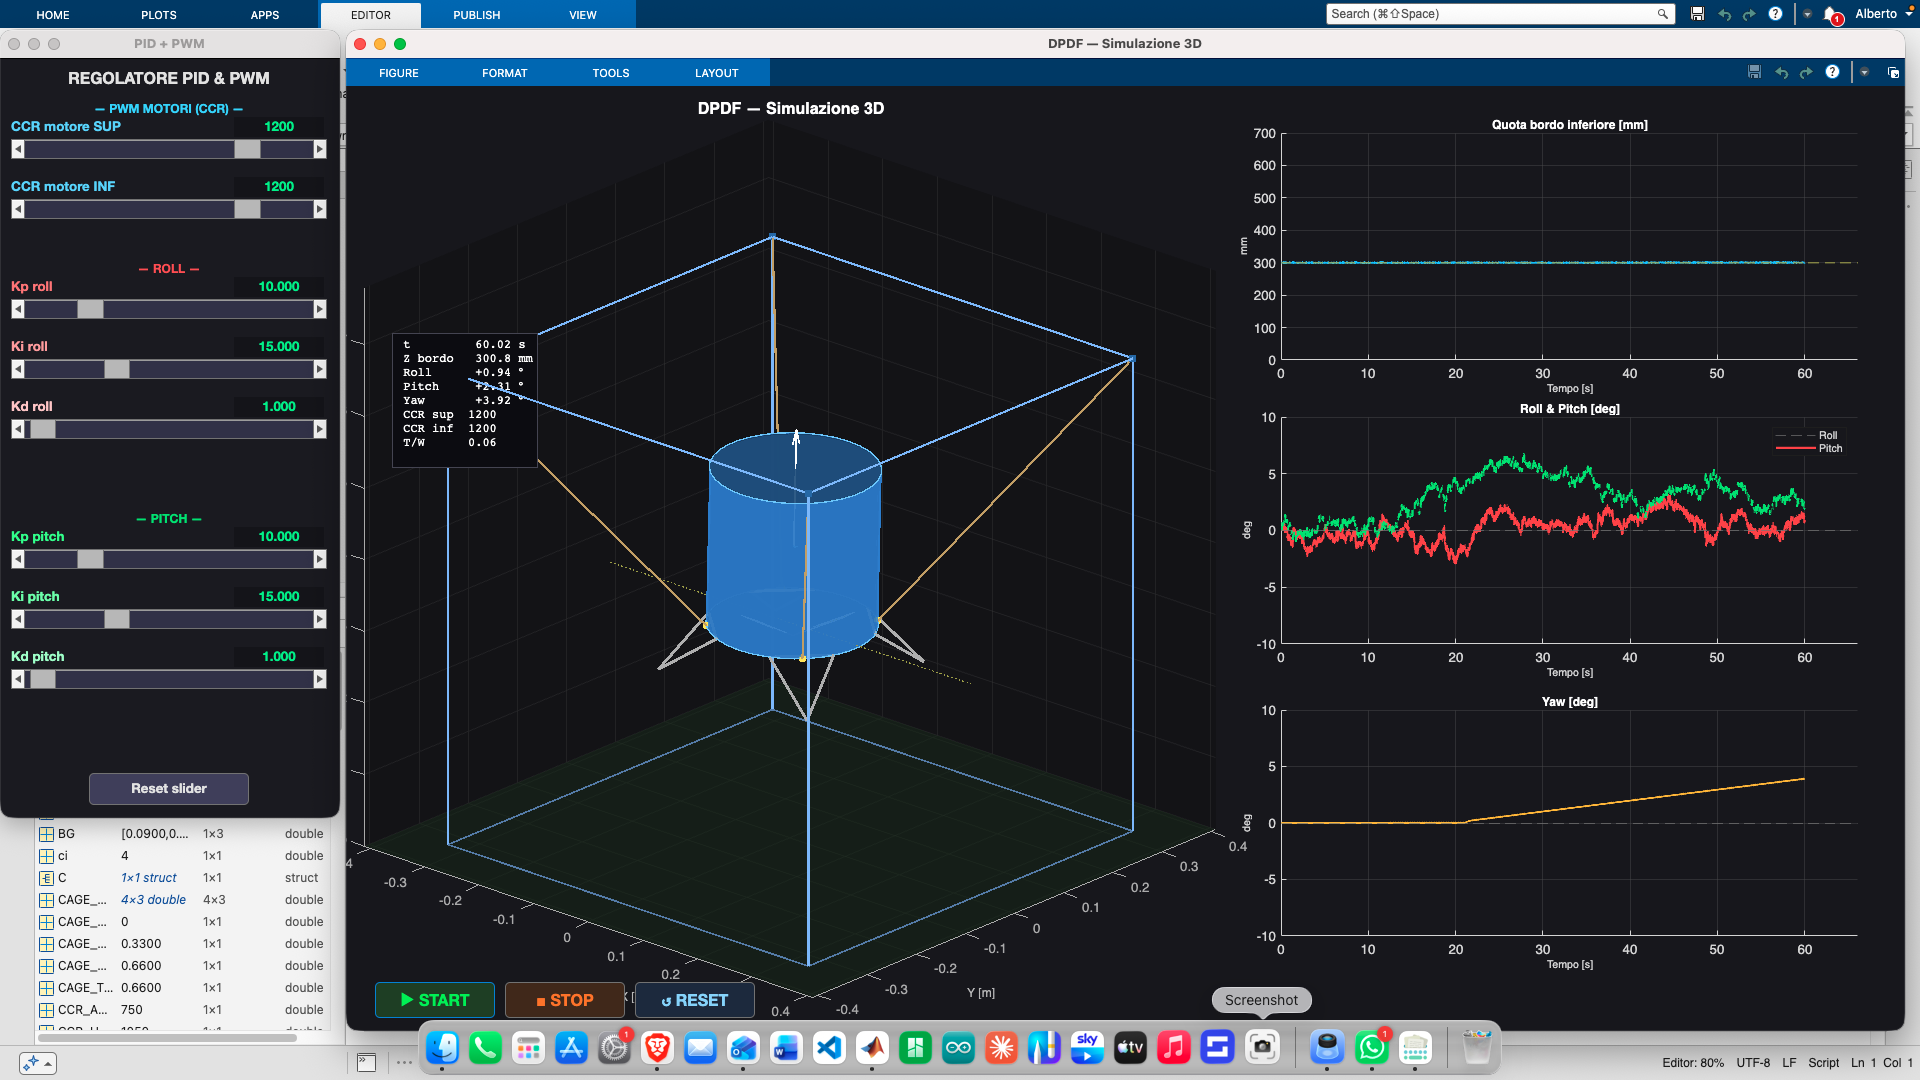
\includegraphics[width=0.95\textwidth]{figures/06_simulazione/screenshot_simulatore.png}
		\caption{Risposta temporale del DPDF nel simulatore (sessione di 60 [s], $CCR = 1050$, PID attivo) con parametri PID in configurazione di sicurezza. In alto: quota del bordo inferiore del cilindro, che si assesta in tensione sulle funi a circa 275 mm dal pavimento della gabbia. Al centro: angoli di \textit{roll} (linea rossa) e \textit{pitch} (linea tratteggiata verde), che vengono mantenuti prossimi allo zero dall'azione dei due PID. In basso: angolo di \textit{yaw}}
		\label{fig:simulazione_hover}
	\end{figure}
	
	I risultati osservati possono essere riassunti nei tre punti seguenti.
	\begin{itemize}
		\item \textbf{Il drone permane nella configurazione vincolata}, sostenuto dalle quattro funi che restano in tensione per l'intera durata della prova. La quota del bordo inferiore si stabilizza intorno a $275$ [mm] dal pavimento della gabbia, valore corrispondente alla configurazione di equilibrio meccanico in cui la componente verticale della tensione delle funi compensa la differenza tra peso del velivolo e spinta dei motori. Coerentemente con quanto anticipato nella Sezione~\ref{sec:modello_spinta_flap}, la spinta complessiva è insufficiente per produrre il decollo libero.
		\item \textbf{L'azione dei regolatori PID converge correttamente}. Gli angoli di \textit{roll} e \textit{pitch}, dopo un breve transitorio iniziale dovuto al momento ribaltante generato dall'eccentricità del baricentro, vengono riportati e mantenuti in un intorno dello zero per l'intera durata della prova. Le oscillazioni residue sono di ampiezza contenuta (dell'ordine di pochi gradi picco-picco) e non mostrano alcuna tendenza alla divergenza né segni di \textit{chattering} sugli attuatori.
		\item \textbf{L'\textit{yaw} resta sostanzialmente fermo}, coerentemente con il fatto che il simulatore non include una sollecitazione differenziale tra i due motori. Eventuali piccoli scostamenti sono dovuti alla componente non perfettamente compensata dei momenti torcenti delle due eliche, che il modello include in forma semplificata.
	\end{itemize}
	
	Il simulatore fornisce dunque due indicazioni complementari, entrambe di valore. Da un lato \textbf{conferma la validità della legge di controllo PID} sintetizzata nel Capitolo~\ref{ch:modello}, mostrando che i regolatori sono in grado di stabilizzare l'assetto del velivolo in presenza dei principali disturbi non lineari (eccentricità del baricentro, accoppiamento con il vincolo elastico). Dall'altro \textbf{conferma il deficit di spinta} che impedisce il volo libero: nessuna combinazione dei guadagni testati produce il decollo, e questo non è un limite dei regolatori ma una caratteristica intrinseca della catena propulsiva nella configurazione attuale. Le cause di tale deficit e le possibili strade per superarlo sono analizzate in dettaglio nel Capitolo~\ref{ch:conclusioni}.
	
%--------------------------------------------------------------
	\section{De-rating dei guadagni per il transfer al prototipo fisico}
	\label{sec:derating}
	
	I guadagni sintetizzati da \texttt{pidtune} sul modello LTI identificato (Tabella~\ref{tab:guadagni_pid}) costituiscono il punto di partenza teorico ottimale. Tuttavia, nel passaggio dal modello al sistema fisico intervengono fattori non modellati che possono favorire l'insorgenza di oscillazioni ad alta frequenza (\textit{chattering}) sugli attuatori: i giochi meccanici dei servomotori \textit{Hitec HS-82MG}, l'attrito statico dei perni dei \textit{flap}, le piccole non-linearità della catena ESC--motore, e il rumore residuo dell'IMU.
	
	Per il primo collaudo sul prototipo fisico si è scelto di adottare una configurazione di sicurezza, ottenuta arrotondando in modo conservativo i guadagni del modello LTI rispetto ai valori sintetizzati nel Capitolo~\ref{ch:modello}. I valori adottati, distinti per i due assi di assetto, sono riportati in Tabella~\ref{tab:guadagni_derated}.
	
	\begin{table}[H]
		\centering
		\begin{tabular}{lcc}
			\toprule
			\textbf{Parametro} & \textbf{Asse di Roll} & \textbf{Asse di Pitch} \\
			\midrule
			$K_{p,\text{safe}}$ & 15.0 & 10.0 \\
			$K_{i,\text{safe}}$ & 40.0 & 11.0 \\
			$K_{d,\text{safe}}$ & 1.0  & 2.0  \\
			\bottomrule
		\end{tabular}
		\caption{Guadagni PIDF adottati per il primo collaudo sul prototipo fisico, distinti per i due assi di controllo}
		\label{tab:guadagni_derated}
	\end{table}
	
	L'asimmetria tra i due assi --- $K_p$ più elevato e $K_i$ significativamente più aggressivo sul \textit{roll} rispetto al \textit{pitch} --- riflette quella già emersa nella sintesi automatica di \texttt{pidtune} (Tabella~\ref{tab:guadagni_pid}), ed è imputabile alla differente struttura dei modelli identificati sui due assi: un secondo ordine con uno zero per il \textit{roll} e un terzo ordine con uno zero per il \textit{pitch}, con guadagni statici di modulo differente. L'azione integrale più forte sul \textit{roll} è dunque necessaria per compensare un guadagno statico più piccolo, mentre il valore più elevato di $K_d$ sul \textit{pitch} contribuisce a smorzare la dinamica leggermente più oscillante predetta dal modello del terzo ordine.
	
	Questi valori sono stati prima validati nel simulatore (producendo la risposta mostrata in Figura~\ref{fig:simulazione_hover}) e successivamente impiegati come punto di partenza nel firmware. La pratica dell'arrotondamento conservativo è una scelta metodologica coerente con la prudenza richiesta nella validazione di sistemi non lineari: i guadagni più aggressivi suggeriti da \texttt{pidtune} possono essere reintrodotti incrementalmente in fase di taratura fine sul prototipo, una volta acquisita confidenza con il comportamento reale del sistema.
	%--------------------------------------------------------------
	\section{Limiti del simulatore e relazione con i capitoli successivi}
	\label{sec:limiti_sim}
	
	Il simulatore tridimensionale qui descritto è uno strumento di verifica utile e fedele entro le ipotesi di costruzione, ma non è privo di limiti. È opportuno enumerarli esplicitamente, sia per circoscrivere la portata dei risultati ottenuti sia per indicare possibili direzioni di sviluppo.
	\begin{itemize}
		\item \textbf{Modello aerodinamico semplificato}: l'azione dei \textit{flap} è descritta da una singola costante $K_\text{aer}$, che racchiude in un parametro empirico l'intero comportamento della superficie aerodinamica. Effetti come la dipendenza dall'angolo di incidenza, lo stallo dinamico e l'interazione con la scia delle eliche non sono modellati esplicitamente.
		\item \textbf{Modello di spinta calibrato a posteriori}: il profilo di \textit{throttle}~\eqref{eq:profilo_throttle} riproduce il comportamento osservato della catena propulsiva nella configurazione attuale, ma non costituisce un modello propulsivo predittivo. Una modifica significativa del sistema (per esempio sostituzione di motori o eliche) richiederebbe una nuova calibrazione sperimentale.
		\item \textbf{Geometria del vincolo idealizzata}: le funi sono modellate come elementi monodimensionali visco-elastici puri, senza considerare effetti come l'attrito sull'ancoraggio, la massa propria della corda o eventuali oscillazioni trasversali.
		\item \textbf{Integratore esplicito}: l'utilizzo di un'integrazione di Eulero esplicita, anche se mitigata dal \textit{sub-stepping}, è meno robusta di metodi impliciti più sofisticati nei confronti dei sistemi rigidi (\textit{stiff}). Un'integrazione di tipo Runge-Kutta del quarto ordine o uno schema implicito potrebbero ulteriormente migliorare la fedeltà numerica, in particolare in presenza di alte rigidezze delle funi.
	\end{itemize}
	
	Pur con questi limiti, il simulatore ha svolto efficacemente il ruolo di banco di prova \textit{a basso rischio} per i regolatori sintetizzati nel Capitolo~\ref{ch:modello}, e ha contribuito significativamente alla comprensione qualitativa della dinamica del prototipo. La sua principale conferma, ribadita anche dai test reali, è che il \textbf{deficit di spinta dell'attuale catena propulsiva preclude il volo libero del velivolo}, indipendentemente dalla qualità del controllo. L'analisi dettagliata delle cause di questa limitazione e le proposte per superarla sono l'oggetto del prossimo capitolo.
	
	%%%%%%%%%%%%%%%%%%%%%%%%%%%%%%%%%%%%%%%%%%%%%%%%%%%%%%%%%%%%%%%%%%%%
	%             CAPITOLO 7 - CONCLUSIONI E SVILUPPI FUTURI
	%%%%%%%%%%%%%%%%%%%%%%%%%%%%%%%%%%%%%%%%%%%%%%%%%%%%%%%%%%%%%%%%%%%%
	\chapter{Conclusioni e Sviluppi Futuri}
	\label{ch:conclusioni}
	
	Il lavoro descritto in questo documento ha condotto allo sviluppo di un'infrastruttura completa per la caratterizzazione e il controllo del prototipo \textit{Double Propeller Ducted-Fan (DPDF)}: l'intera struttura meccanica è stata riprogettata e ristampata in 3D, è stata implementata un'architettura firmware \textit{event-driven} sulla scheda STM32 NUCLEO-H745ZI-Q, è stato realizzato un canale di telemetria bidirezionale a 230\,400 [bps] in grado di campionare lo stato cinematico del velivolo a 50 [Hz], sono state identificate le funzioni di trasferimento dei singoli assi di assetto tramite \texttt{tfest} ed è stato costruito un simulatore fisico tridimensionale \textit{grey-box} in MATLAB per la verifica dei regolatori in ambiente controllato.
	
	Tutti questi elementi, presi singolarmente e nel loro insieme, costituiscono un risultato tangibile del progetto. Resta tuttavia un dato di fatto che il prototipo, nella configurazione hardware attuale, \textbf{non è stato in grado di sostenere il volo libero}: tutte le prove sperimentali sono state condotte con il drone vincolato all'interno della gabbia di sicurezza, e nei tentativi di valutare la spinta in configurazione svincolata il velivolo si è limitato a sollevarsi parzialmente per poi tornare in contatto con il banco di prova. Il presente capitolo è dunque dedicato a un'analisi critica delle cause di questo limite e a una proposta di linee guida per il superamento nelle iterazioni future del progetto. L'obiettivo è duplice: rendere conto in modo trasparente del comportamento osservato, ed estrarre dalle limitazioni incontrate indicazioni concrete per chi si occuperà del seguito del progetto.
	
	%--------------------------------------------------------------
	\section{Analisi critica delle cause di mancato volo libero}
	\label{sec:analisi_cause}
	
	Le cause del mancato volo libero sono state isolate attraverso il confronto incrociato di tre fonti di evidenza: l'analisi analitica delle caratteristiche fisiche della catena propulsiva, l'osservazione del comportamento del simulatore (Capitolo~\ref{ch:simulazione}) e i test sul prototipo fisico. Le cinque criticità identificate, presentate di seguito in ordine di importanza decrescente rispetto al volo libero, contribuiscono in maniera congiunta a precludere il sollevamento autonomo del velivolo.
	
	\subsection{Verifica analitica del deficit di spinta}
	\label{sec:verifica_spinta}
	La prima e più rilevante delle limitazioni del prototipo riguarda il \textbf{sistema propulsivo}. In questa sezione si conduce una verifica quantitativa volta a stabilire se la combinazione propulsiva adottata --- motore \textit{Turnigy SK3-3536 1400~KV} ed elica \textit{APC 9$\times$4.5} --- sia in grado di generare la spinta necessaria al sollevamento del velivolo. L'analisi confronta la spinta massima erogabile dai due motori con la forza peso del sistema, prima attraverso un limite teorico basato sulla potenza disponibile e successivamente attraverso una stima fondata su dati di spinta misurati sperimentalmente per la medesima famiglia di eliche.
	
	\subsubsection*{Condizione di hovering e forza peso}
	La condizione necessaria affinché il velivolo possa sollevarsi da terra e mantenere una quota costante impone che la spinta totale generata dai due motori superi la forza peso del sistema:
	\begin{equation}
		T_\text{tot} > F_p = m \cdot g
		\label{eq:condizione_hovering}
	\end{equation}
	Considerando la massa complessiva del velivolo assemblato $m = 2.2$ [kg] e l'accelerazione di gravità $g = 9.81$ [m/s$^2$], la forza peso da vincere risulta:
	\begin{equation}
		F_p = 2.2 \cdot 9.81 = 21.58\ \text{[N]}
		\label{eq:forza_peso}
	\end{equation}
	Tale valore costituisce la soglia minima di spinta che il sistema propulsivo deve essere in grado di erogare per garantire il volo libero.
	
	\subsubsection*{Limite teorico imposto dalla potenza disponibile}
	Un primo limite superiore alla spinta ottenibile può essere ricavato dalla teoria del disco attuatore, indipendentemente dal regime di rotazione effettivamente raggiunto dal motore. Per un disco attuatore di area $A$ che elabora una potenza $P$, la spinta massima teorica in condizioni statiche vale:
	\begin{equation}
		T_\text{id} = \left( 2 \, \rho \, A \, P^2 \right)^{1/3}
		\label{eq:disco_attuatore}
	\end{equation}
	dove $\rho = 1.225$ [kg/m$^3$] è la densità dell'aria e $A = \pi (D/2)^2$ è l'area spazzata dall'elica. Con un diametro $D = 0.2286$ [m] (elica \textit{APC 9$\times$4.5}) si ottiene:
	\begin{equation}
		A = \pi \cdot (0.1143)^2 = 0.04105\ \text{[m$^2$]}
		\label{eq:area_elica}
	\end{equation}
	Assumendo la potenza massima di targa del motore $P = 590$ [W], la spinta ideale del singolo motore risulta:
	\begin{equation}
		T_\text{id} = \left( 2 \cdot 1.225 \cdot 0.04105 \cdot 590^2 \right)^{1/3} \approx 32.7\ \text{[N]}
		\label{eq:spinta_ideale}
	\end{equation}
	Questo valore rappresenta un limite puramente ideale, ottenuto ipotizzando un'efficienza propulsiva unitaria. Le eliche reali presentano una \textit{Figure of Merit (FM)} tipicamente compresa tra 0.5 e 0.7; assumendo un valore realistico $\text{FM} = 0.6$ e tenendo conto della riduzione di efficienza del motore inferiore dovuta al \textit{downwash} (fattore 0.7), la spinta totale teorica si riduce a:
	\begin{equation}
		T_\text{tot}^\text{teorico} = \text{FM} \cdot T_\text{id} \cdot (1 + 0.7) = 0.6 \cdot 32.7 \cdot 1.7 \approx 33.3\ \text{[N]}
		\label{eq:spinta_teorica}
	\end{equation}
	Tale risultato indica che, qualora i motori operassero effettivamente alla potenza di picco di 590 [W], la spinta disponibile sarebbe teoricamente sufficiente al sollevamento. Come si mostrerà nel paragrafo seguente, tuttavia, tale condizione di funzionamento non viene mai raggiunta nelle reali condizioni operative del sistema.
	
	\subsubsection*{Limite operativo reale e dati sperimentali dell'elica}
	La potenza di picco di 590 [W] è erogabile dal motore unicamente al regime di rotazione massimo a vuoto, pari a:
	\begin{equation}
		\text{RPM}_\text{vuoto} = K_V \cdot V = 1400 \cdot 14.8 = 20\,720\ \text{[RPM]}
		\label{eq:rpm_vuoto}
	\end{equation}
	Una volta calettata l'elica, però, la coppia aerodinamica resistente opposta da quest'ultima riduce drasticamente il regime di rotazione effettivamente raggiungibile. Poiché la potenza assorbita da un'elica scala con il cubo della velocità di rotazione ($P \propto n^3$), il motore si stabilizza, in condizioni statiche, a un regime sensibilmente inferiore a quello a vuoto.
	
	I dati di letteratura specialistica, tra cui quelli raccolti dallo \textit{UIUC Propeller Database}~\cite{uiuc_propeller_db} per eliche APC della stessa famiglia (9$\times$4.7, geometricamente affine alla 9$\times$4.5 impiegata sul prototipo), indicano un regime statico tipico per motori di questa classe nell'intorno di 9\,000 [RPM], corrispondente a:
	\begin{equation}
		n = \frac{9\,000}{60} = 150\ \text{[giri/s]}
		\label{eq:rpm_statico}
	\end{equation}
	Il medesimo database fornisce inoltre un coefficiente di spinta statico misurato $C_T \approx 0.105$ (definito secondo la convenzione $C_T = T / (\rho \, n^2 \, D^4)$). Questo valore è notevolmente inferiore a quello impiegato nei modelli puramente ideali ($C_T \approx 0.2$) ed è decisamente più rappresentativo del comportamento reale dell'elica in condizioni statiche.
	
	La spinta del singolo motore superiore (operante in aria indisturbata) risulta quindi:
	\begin{equation}
		T_\text{up} = C_T \cdot \rho \cdot n^2 \cdot D^4 = 0.105 \cdot 1.225 \cdot 150^2 \cdot 0.2286^4 \approx 7.9\ \text{[N]}
		\label{eq:spinta_singolo}
	\end{equation}
	Applicando il fattore di efficienza dovuto al \textit{downwash} sul motore inferiore (fattore di scia pari a 0.7), la spinta totale erogata dal sistema vale:
	\begin{equation}
		T_\text{tot}^\text{reale} = T_\text{up} \cdot (1 + 0.7) = 7.9 \cdot 1.7 \approx 13.4\ \text{[N]}
		\label{eq:spinta_reale}
	\end{equation}
	
	\subsubsection*{Confronto e conclusione}
	Confrontando la spinta totale realisticamente disponibile della relazione~\eqref{eq:spinta_reale} con la forza peso~\eqref{eq:forza_peso} si ottiene:
	\begin{equation}
		T_\text{tot}^\text{reale} \approx 13.4\ \text{[N]} < F_p = 21.58\ \text{[N]}
		\label{eq:deficit}
	\end{equation}
	La spinta disponibile risulta dunque inferiore alla forza peso di circa il 38\%, da cui si conclude analiticamente che \textbf{il velivolo, nella configurazione propulsiva adottata, non è in grado di sollevarsi dal suolo}.
	
	È opportuno sottolineare che la stima~\eqref{eq:spinta_reale} costituisce uno scenario ottimistico. Il deficit di spinta reale è verosimilmente superiore, poiché non sono stati considerati gli effetti di ostruzione aerodinamica e l'attrito della struttura del condotto, le perdite meccaniche complessive e le inefficienze degli ESC. La coerenza con le osservazioni sperimentali e con la calibrazione del simulatore (Capitolo~\ref{ch:simulazione}, in cui la spinta massima del modello è stata fissata a circa $13 \div 14$ [N] proprio sulla base delle misurazioni reali) conferma la correttezza dell'analisi.
	
	La causa fisica del fenomeno risiede nel netto \textbf{sottodimensionamento dell'accoppiamento motore--elica}: la combinazione di un motore ad elevato $K_V$ (1400 [RPM/V]), ottimizzato per alti regimi di rotazione, con un'elica di piccolo diametro (9~pollici) privilegia la velocità di rotazione a discapito della spinta statica erogata. Per ottenere una spinta adeguata al sollevamento di una massa di 2.2 [kg] sarebbe necessario adottare eliche di diametro maggiore (nell'intorno di $12 \div 15$~pollici) abbinate a motori a $K_V$ inferiore e coppia più elevata, oppure incrementare il numero di unità propulsive.
	
	\subsection{Distribuzione delle masse ed elevata inerzia perimetrale}
	\label{sec:distribuzione_masse}
	La seconda criticità, indipendente dalla prima ma con essa concorrente, riguarda la distribuzione geometrica delle masse all'interno del prototipo. La scelta progettuale di collocare l'intera infrastruttura hardware --- comprendente la scheda di controllo \textit{NUCLEO}, i due convertitori di tensione \textit{DFRobot}, la \textit{Power Distribution Board}, i due ESC \textit{Turnigy Plush 40A} e, soprattutto, il doppio pacco batteria \textit{Tattu LiPo 4S} --- lungo la superficie cilindrica esterna del condotto introduce un effetto collaterale meccanico significativo.
	
	Dal punto di vista della fisica dei corpi rigidi, distribuire componenti ad alta densità di massa sul perimetro esterno allontana la materia dall'asse di rotazione geometrico, incrementando i momenti d'inerzia principali del velivolo ($I_{xx}$ e $I_{yy}$). Un valore elevato di inerzia richiede coppie di controllo più elevate per imprimere le accelerazioni angolari necessarie a stabilizzare un sistema intrinsecamente instabile come il \textit{ducted-fan}. Questo effetto, da solo, non sarebbe sufficiente a precludere il volo libero in presenza di una catena propulsiva adeguata, ma in combinazione con le altre criticità contribuisce a rendere il problema di controllo molto più impegnativo del necessario.
	
	\subsection{Eccentricità del baricentro e momento ribaltante gravitazionale}
	\label{sec:eccentricita_cg}
	I test di identificazione hanno evidenziato la presenza di accoppiamenti dinamici (\textit{cross-coupling}) e sbilanciamenti statici costanti, riconducibili a un disallineamento del centro di gravità rispetto all'asse di spinta teorico pari a $d_{cg,x} = 2.8$ [mm] e $d_{cg,y} = 3.8$ [mm]. Sebbene tali valori possano apparire trascurabili in scala assoluta, in un velivolo intubato a singolo condotto essi generano un \textbf{momento ribaltante destabilizzante} non appena i motori principali erogano la spinta verticale $F_t$:
	\begin{equation}
		M_\text{gravity} = F_t \cdot d_{cg}
		\label{eq:momento_gravity}
	\end{equation}
	Poiché il baricentro si trova geometricamente al di sopra del punto di applicazione delle forze aerodinamiche correttive dei \textit{flap}, il sistema si comporta come un pendolo inverso accelerato dalla gravità, la cui tendenza al ribaltamento cresce linearmente con la spinta richiesta. In altre parole, paradossalmente, maggiore è la potenza fornita ai motori, maggiore è anche il momento destabilizzante che il sistema di controllo deve compensare.
	
	\subsection{Deficit di autorità di controllo dei flap}
	\label{sec:autorita_controllo}
	Una terza criticità riguarda l'\textbf{autorità di controllo} (\textit{control authority}) offerta dai due \textit{flap} direzionali posti alla base del condotto. A differenza dei multirotori convenzionali, che generano momenti di ripristino imponenti variando differenzialmente la velocità dei rotori posti alle estremità di bracci meccanici estesi, il DPDF si affida unicamente alla deviazione del getto d'aria discendente.
	
	Il momento correttivo massimo generabile dai \textit{flap} è strutturalmente limitato dal piccolo braccio aerodinamico equivalente $K_\text{aer} = 0.0025$ [m/deg] e dalla superficie ridotta delle alette stesse, secondo la legge:
	\begin{equation}
		\max\!\left| M_\text{flap} \right| = \max\!\left| f_\text{flap} \right| \cdot K_\text{aer} \cdot F_t
		\label{eq:autorita_flap}
	\end{equation}
	Sotto l'effetto della saturazione fisica imposta a $\pm 30\degree$ per preservare l'integrità dei servomotori \textit{Hitec HS-82MG}, l'azione correttiva massima erogabile dai \textit{flap} risulta dello stesso ordine di grandezza --- e in alcune condizioni inferiore --- del momento destabilizzante indotto dal disallineamento del baricentro. Il sistema di attuazione si trova quindi a operare costantemente in prossimità della saturazione geometrica, con margine di controllo ridotto per fronteggiare disturbi aerodinamici aggiuntivi.
	
	\subsection{L'effetto mascheramento del vincolo}
	\label{sec:masking_effect}
	Un'osservazione metodologica importante riguarda il \textbf{motivo per cui il drone è apparso stabile} sia nel simulatore sia nei test in laboratorio, in contrasto con la previsione di mancato volo libero. All'interno della gabbia di sicurezza, le quattro funi disposte ai vertici superiori agiscono come elementi visco-elastici stabilizzanti, secondo il modello di Kelvin-Voigt descritto nel Capitolo~\ref{ch:simulazione}.
	
	Quando il drone tende a inclinarsi per via del baricentro eccentrico o di un disturbo aerodinamico, le funi del lato opposto si caricano in tensione, esercitando una forza di richiamo:
	\begin{equation}
		F_\text{fune} = K_\text{rope} \cdot \Delta L + D_\text{rope} \cdot v_\text{assiale}
		\label{eq:forza_fune_cap7}
	\end{equation}
	Questa forza, applicata in un punto distante dal centro di massa del drone, genera un \textbf{momento stabilizzante esogeno} che si somma all'azione correttiva dei \textit{flap}. Il vincolo meccanico esterno, pensato come misura di sicurezza, ha così \textit{mascherato} il problema di stabilità: nei test vincolati la combinazione di PID + funi è sufficiente a mantenere il drone in posizione, mentre nel volo libero verrebbe a mancare proprio l'energia di ripristino delle funi --- la più potente delle due componenti --- lasciando il sistema in balìa di coppie aerodinamiche non sufficientemente compensate.
	
	Questa osservazione ha un'importanza non solo descrittiva ma anche \textit{metodologica}, per gli sviluppi futuri: il banco di prova vincolato è uno strumento utile e necessario per la fase di taratura iniziale e per le prove di sicurezza, ma non costituisce di per sé una prova della stabilità del velivolo in volo libero. Quest'ultima richiede inevitabilmente un test in configurazione svincolata, a fronte del quale però è imprescindibile aver prima risolto le criticità strutturali identificate nelle sezioni precedenti.
	
	%--------------------------------------------------------------
	\section{Sviluppi futuri e linee guida per la riprogettazione}
	\label{sec:sviluppi_futuri}
	
	L'analisi delle cause condotta nella Sezione~\ref{sec:analisi_cause} suggerisce con chiarezza le direzioni di intervento per le iterazioni future del progetto. Le seguenti linee guida sono presentate in ordine di priorità decrescente, coerentemente con l'impatto atteso sulla capacità di volo libero del velivolo.
	
	\subsection{Riprogettazione del sistema propulsivo}
	\label{sec:riprogettazione_propulsiva}
	La priorità assoluta è il superamento del deficit di spinta documentato nella Sezione~\ref{sec:verifica_spinta}. La via maestra è la \textbf{sostituzione della combinazione motore--elica} con una catena propulsiva dimensionata correttamente per la massa del velivolo:
	\begin{itemize}
		\item \textbf{Adozione di eliche di diametro maggiore}, nell'intorno dei $12 \div 15$ pollici. Il coefficiente di spinta statico aumenta con la quarta potenza del diametro (a parità di altre condizioni), e già un passaggio a un'elica da 12 pollici raddoppierebbe approssimativamente la spinta erogabile a parità di regime di rotazione.
		\item \textbf{Accoppiamento con motori a $K_V$ ridotto} (tipicamente nell'intervallo $700 \div 900$ [RPM/V]), caratterizzati da coppia più elevata e regimi di rotazione contenuti, più adatti al pilotaggio di eliche di grande diametro.
		\item \textbf{In alternativa, aumento del numero di unità propulsive}, ad esempio con una configurazione a quattro motori coassiali (due coppie controrotanti) anziché due. Questa soluzione moltiplicherebbe la spinta totale a parità di tipologia di motore-elica, ma introdurrebbe complessità ulteriore nel \textit{mixer} di controllo.
	\end{itemize}
	Indipendentemente dalla scelta specifica, il dimensionamento futuro dovrà essere preceduto da una verifica analitica del tipo riportato nella Sezione~\ref{sec:verifica_spinta}, in modo da non incorrere nuovamente in deficit di spinta non riconosciuti in fase di progettazione.
	
	\subsection{Centratura e accostamento delle masse}
	\label{sec:centratura_masse}
	Risolto il problema di spinta, la seconda priorità è la riduzione dell'inerzia perimetrale e l'azzeramento dell'eccentricità del baricentro. La direzione di intervento è la \textbf{riprogettazione del layout interno} del drone:
	\begin{itemize}
		\item Eliminazione di ogni componente dal perimetro esterno del cilindro;
		\item Alloggiamento della scheda di controllo, degli ESC e della batteria in un \textit{mozzo centrale} coassiale all'asse di spinta, protetto dal flusso d'aria da un involucro aerodinamico;
		\item Bilanciamento sperimentale del prototipo finale tramite verifica diretta dei momenti residui, prima delle prove di volo.
	\end{itemize}
	Questa modifica ridurrebbe significativamente $I_{xx}$ e $I_{yy}$ (con conseguente aumento della reattività ai comandi di assetto) e abbatterebbe il momento ribaltante gravitazionale che è oggi il principale disturbo statico osservato.
	
	\subsection{Aumento dell'autorità di controllo}
	\label{sec:aumento_autorita}
	A complemento delle prime due linee guida, si rende necessario incrementare l'autorità correttiva del sistema di controllo. Due strade sono percorribili:
	\begin{itemize}
		\item \textbf{Aumento dell'area efficace dei \textit{flap}} o sostituzione con superfici aerodinamiche più estese, eventualmente affiancate a un secondo stadio di \textit{flap} ruotati di $90\degree$ per ridurre l'accoppiamento tra i due assi.
		\item \textbf{Abbandono dell'attuazione a \textit{flap} fissi} in favore di un sistema a \textbf{vettorizzazione della spinta} (\textit{thrust vectoring}): l'intero blocco motore inferiore viene inclinato dinamicamente tramite un anello cardanico (\textit{gimbal ring layout}). Questa soluzione, già adottata su numerosi velivoli a propulsione intubata, fornisce un'autorità di controllo significativamente superiore a quella delle deflessioni di flusso.
	\end{itemize}
	
	\subsection{Riduzione del peso strutturale}
	\label{sec:riduzione_peso}
	Infine, la riduzione del peso complessivo del velivolo agisce favorevolmente su tutte le criticità sopra menzionate: riduce la spinta richiesta per il sollevamento, riduce le inerzie, e amplifica i margini operativi del sistema di controllo. Direzioni di intervento:
	\begin{itemize}
		\item Sostituzione del PLA delle stampe 3D con strutture alveolari in fibra di carbonio o filamenti compositi alleggeriti (PLA-CF, PA-CF) per i componenti strutturali principali;
		\item Verifica della reale necessità del doppio pacco batteria e valutazione di un'unica batteria di pari capacità ma minor peso complessivo (la duplicazione introduce ridondanza ma anche zavorra);
		\item Razionalizzazione del cablaggio e dell'elettronica accessoria.
	\end{itemize}
	Un obiettivo realistico, raggiungibile con questi accorgimenti, è una massa complessiva attorno a $1.5 \div 1.7$ [kg], che ridurrebbe la forza peso da circa 21.6 [N] a circa $14.7 \div 16.7$ [N] e --- in combinazione con la riprogettazione propulsiva descritta nella Sezione~\ref{sec:riprogettazione_propulsiva} --- porterebbe il sistema in una regione operativa nettamente più favorevole al volo libero.
	
	%--------------------------------------------------------------
	\section{Considerazioni conclusive}
	\label{sec:considerazioni_finali}
	
	Il presente lavoro non ha condotto al volo libero del prototipo, ma ha prodotto un risultato in larga parte indipendente da questo obiettivo: una \textbf{piattaforma metodologica completa} per la caratterizzazione, l'identificazione e la simulazione del \textit{DPDF}, fondata su strumenti riutilizzabili e direttamente trasferibili alle future iterazioni del progetto. In particolare, l'infrastruttura di telemetria a 50 [Hz], lo \textit{script} di acquisizione automatizzato, lo \textit{script} di identificazione \texttt{Identify\_and\_tune.m}, il simulatore tridimensionale \texttt{Sim.m} e la procedura di sintesi automatica dei regolatori PIDF costituiscono un patrimonio software direttamente impiegabile sulla prossima generazione del prototipo, una volta risolte le criticità hardware identificate.
	
	A questo si aggiunge un risultato di natura analitica non meno significativo: la verifica quantitativa, esposta nella Sezione~\ref{sec:verifica_spinta}, secondo cui la configurazione propulsiva attuale è strutturalmente insufficiente per il sollevamento del velivolo. Questa conclusione, raggiunta attraverso un confronto rigoroso tra la spinta teorica e quella reale misurata su eliche della stessa famiglia, fornisce un'indicazione tecnica precisa per la riprogettazione futura, sottraendo all'incertezza il dimensionamento della catena propulsiva.
	
	Riteniamo che la combinazione di questi due esiti --- una pipeline di sviluppo metodologicamente solida e un'analisi che spiega in modo trasparente i limiti incontrati --- rappresenti un contributo utile per chi proseguirà il lavoro sul \textit{Double Propeller Ducted-Fan}, e costituisca il punto di partenza naturale per un prototipo di nuova generazione che, recependo le indicazioni qui formulate, possa finalmente trasferire al volo libero il sistema di controllo qui sviluppato.
    %%%%%%%%%%%%%%%%%%%%%%%%%%%%%%%%%%%%%%%%%%%%%%%%%%%%%%%%%%%%%%%%%%%%
	%                            BIBLIOGRAFIA
	%%%%%%%%%%%%%%%%%%%%%%%%%%%%%%%%%%%%%%%%%%%%%%%%%%%%%%%%%%%%%%%%%%%%
	\bibliographystyle{ieeetr}
	\bibliography{bibl}
	
\end{document}